%%%%%%%%%%%%%%%%%%%%%%%%%%%%%%%%%%%%%%%%%%%%%%%%%%%%%%%%%%%%%%%%%%%%%%%%
% Uni Duesseldorf
% Lehrstuhl fuer Datenbanken und Informationssysteme
% Vorlage fuer Bachelor-/Masterarbeiten
% Optimiert fuer den Original-Latex-Kompiler LATEX.EXE (LaTeX=>PS=>PDF)
%%%%%%%%%%%%%%%%%%%%%%%%%%%%%%%%%%%%%%%%%%%%%%%%%%%%%%%%%%%%%%%%%%%%%%%%
% Ueberarbeitung für pdflatex (LaTeX=>PDF)
%%%%%%%%%%%%%%%%%%%%%%%%%%%%%%%%%%%%%%%%%%%%%%%%%%%%%%%%%%%%%%%%%%%%%%%%
% Vorlage Changelog:
% 10.09.2015 (Matthias Liebeck): Nummerierung des Inhaltsverzeichnis nun römisch, Beispiel für einen Anhang eingebaut, \raggedbottom hinter sections eingefügt
%%%%%%%%%%%%%%%%%%%%%%%%%%%%%%%%%%%%%%%%%%%%%%%%%%%%%%%%%%%%%%%%%%%%%%%%
%%%% BEGINN EINSTELLUNG FUER DIE ARBEIT. UNBEDINGT ERFORDERLICH! %%%%%%%
%%%%%%%%%%%%%%%%%%%%%%%%%%%%%%%%%%%%%%%%%%%%%%%%%%%%%%%%%%%%%%%%%%%%%%%%
% Geben Sie Ihren Namen hier an:
\newcommand{\bearbeiter}{Robin Bially}

% Geben Sie hier den Titel Ihrer Arbeit an:
\newcommand{\titel}{Wie verbrennt man eine Bildzeitung?}

% Geben Sie das Datum des Beginns und Ende der Bachelorarbeit ein:
\newcommand{\beginndatum}{01. April 2010}
\newcommand{\abgabedatum}{31.~September~2018}

% Geben Sie die Namen des Erst- und Zweitgutachters an:
\newcommand{\erstgutachter}{PD. Dr. Dr. Wilfried Linder}
\newcommand{\zweitgutachter}{niemand}

% Falls Sie die Arbeit zweiseitig ausdrucken wollen,
% benutzen Sie die folgende Zeile mit
% \AN fuer zweiseitigen Druck
% \AUS fuer einseitigen Druck
\newcommand{\zweiseitig}{\AN}

% Falls die Arbeit in englischer Sprache verfasst 
% werden soll, dann benutzen Sie die folgende Zeile mit
% englisch fuer englische Sprache
% deutsch fuer deutsche Sprache
\newcommand{\sprache}{deutsch}

% Hier wird eingestellt, ob es sich bei der Arbeit um eine Bachelor- 
% oder Masterarbeit handelt (unpassendes auskommentieren!):
\newcommand{\arbeit}{Bachelorarbeit}
%~ \newcommand{\arbeit}{Masterarbeit}


%%%%%%%%%%%%%%%%%%%%%%%%%%%%%%%%%%%%%%%%%%%%%%%%%%%%%%%%%%%%%%%%%%%%%%%%
%%%% ENDE EINSTELLUNGEN %%%%%%%%%%%%%%%%%%%%%%%%%%%%%%%%%%%%%%%%%%%%%%%%
%%%%%%%%%%%%%%%%%%%%%%%%%%%%%%%%%%%%%%%%%%%%%%%%%%%%%%%%%%%%%%%%%%%%%%%%

% Die folgende Zeile NICHT EDITIEREN oder loeschen


%%%%%%%%%%%%%%%%%%%%%%%%%%%%%%%%%%%%%%%%%%%%%%%%%%%%%%%%%%%
% Obere Titelmakros. Editieren Sie diese Datei nur, wenn
% Sie sich ABSOLUT sicher sind, was Sie da tun!!!
% (Z.B. zum Abaendern der BA-Vorlage in eine MA-Vorlage)
% Uni Duesseldorf
% Lehrstuhl fuer Datenbanken und Informationssysteme
% Version 2.2 - 2.3.2010
%%%%%%%%%%%%%%%%%%%%%%%%%%%%%%%%%%%%%%%%%%%%%%%%%%%%%%%%%%%
\newcommand{\AN}{twoside}
\newcommand{\AUS}{}
%\newcommand{\englisch}{}
%\newcommand{\deutsch}{\usepackage[german]{babel}}

%% Die folgenden auskommentierten Optionen dienen der automatischen
%% Erkennung des Latex-Kompilers und dem Setzen der davon abhängigen
%% Einstellungen. Bei Problem z.B. mit dem Einbinden von verschiedenen
%% Grafiktypen bei Verwendung von PdfLatex oder Latex, einfach die
%% verschiedenen \usepackage(s) ausprobieren. (Mit diesen Einstellungen
%% funktionierte diese Vorlage bei der Verwenundg von latex.exe als
%% Kompiler bei den meisten Studierenden.)

%\newif\ifpdf \ifx\pdfoutput\undefined
%\pdffalse % we are not running pdflatex
%\else
%\pdfoutput=1 % we are running pdflatex
%\pdfcompresslevel=9 % compression level for text and image;
%\pdftrue \fi

\documentclass[11pt,a4paper, \zweiseitig]{article}



%\usepackage[iso]{umlaute}
\usepackage[utf8x]{inputenc}
\usepackage{palatino} % palatino Schriftart
%\usepackage{makeidx} % um ein Index zu erstellen
\usepackage[nottoc]{tocbibind}
\usepackage[T1]{fontenc} %fuer richtige Trennung bei Umlauten
\usepackage{fancybox} % fuer die Rahmen
\usepackage{shortvrb}
\usepackage{ifthen}
\ifthenelse{\equal{\sprache}{deutsch}}{\usepackage[ngerman]{babel}}{}

\usepackage{a4wide} % ganze A4 Weite verwenden

%\ifpdf
%\usepackage[pdftex,xdvi]{graphicx}
%\usepackage{thumbpdf} %thumbs fuer Pdf
%\usepackage[pdfstartview=FitV]{hyperref} %anklickbares Inhaltsverzeichnis
%\else
%\usepackage[dvips,xdvi]{graphicx}
\usepackage{graphicx}
\usepackage{hyperref} %anklickbares Inhaltsverzeichnis
%\fi

%%%%%%%%%%%%%%%%%%%%%%% Massangaben fuer die Arbeit %%%%%%%%%%%%%%%
\setlength{\textwidth}{15cm}

\setlength{\oddsidemargin}{35mm}
\setlength{\evensidemargin}{25mm}

\addtolength{\oddsidemargin}{-1in}
\addtolength{\evensidemargin}{-1in}

%\makeindex

\begin{document}

%\setcounter{secnumdepth}{4} %Nummerieren bis in die 4. Ebene
%\setcounter{tocdepth}{4} %Inhaltsverzeichnis bis zur 4. Ebene

\pagestyle{headings}

\sloppy % LaTeX ist dann nicht so streng mit der Silbentrennung
%~ \MakeShortVerb{\§}

\parindent0mm
\parskip0.5em


{
\textwidth170mm 
\oddsidemargin30mm 
\evensidemargin30mm 
\addtolength{\oddsidemargin}{-1in}
\addtolength{\evensidemargin}{-1in}

\parskip0pt plus2pt

% Die Raender muessen eventuell fuer jeden Drucker individuell eingestellt
% werden. Dazu sind die Werte fuer die Abstaende `\oben' und `\links' zu
% aendern, die von mir auf jeweils 0mm eingestellt wurden.

%\newlength{\links} \setlength{\links}{10mm}  % hier abzuaendern
%\addtolength{\oddsidemargin}{\links}
%\addtolength{\evensidemargin}{\links}

\begin{titlepage}
\vspace*{-1.5cm}
  \raisebox{17mm}{
    \begin{minipage}[t]{70mm}
      \begin{center}
        %\selectlanguage{german}
        {\Large INSTITUT FÜR INFORMATIK\\}
        {\normalsize
          Datenbanken und Informationssysteme\\
        }
        \vspace{3mm}
        {\small Universitätsstr. 1 \hspace{5ex} D--40225 Düsseldorf\\}
     \end{center}
    \end{minipage}
  }
  \hfill
  
\includegraphics[width=130pt]{bilder/HHU_Logo}
  \vspace{14em}

% Titel
  \begin{center}
      	\baselineskip=55pt
    	\textbf{\huge \titel}
  	 	\baselineskip=0 pt
   \end{center}

  %\vspace{7em}

\vfill

% Autor
  \begin{center}
    \textbf{\Large
      \bearbeiter
    }
  \end{center}

  \vspace{35mm}
 
% Prüfungsordnungs-Angaben
  \begin{center}
    %\selectlanguage{german}
    
%%%%%%%%%%%%%%%%%%%%%%%%%%%%%%%%%%%%%%%%%%%%%%%%%%%%%%%%%%%%%%%%%%%%%%%%%
% Ja, richtig, hier kann die BA-Vorlage zur MA-Vorlage gemacht werden...
% (nicht mehr nötig!)
%%%%%%%%%%%%%%%%%%%%%%%%%%%%%%%%%%%%%%%%%%%%%%%%%%%%%%%%%%%%%%%%%%%%%%%%%
    {\Large \arbeit}

    \vspace{2em}

    \begin{tabular}[t]{ll}
      Beginn der Arbeit:& \beginndatum \\
      Abgabe der Arbeit:& \abgabedatum \\
      Gutachter:         & \erstgutachter \\
                         & \zweitgutachter \\
    \end{tabular}
  \end{center}

\end{titlepage}

}

%%%%%%%%%%%%%%%%%%%%%%%%%%%%%%%%%%%%%%%%%%%%%%%%%%%%%%%%%%%%%%%%%%%%%
\clearpage
\begin{titlepage}
  ~                % eine leere Seite hinter dem Deckblatt
\end{titlepage}
%%%%%%%%%%%%%%%%%%%%%%%%%%%%%%%%%%%%%%%%%%%%%%%%%%%%%%%%%%%%%%%%%%%%%
\clearpage
\begin{titlepage}
\vspace*{\fill}

\section*{Erklärung}

%%%%%%%%%%%%%%%%%%%%%%%%%%%%%%%%%%%%%%%%%%%%%%%%%%%%%%%%%%%
% Und hier ebenfalls ggf. BA durch MA ersetzen...
% (Auch nicht mehr nötig!)
%%%%%%%%%%%%%%%%%%%%%%%%%%%%%%%%%%%%%%%%%%%%%%%%%%%%%%%%%%%

Hiermit versichere ich, dass ich diese \arbeit~
selbstständig verfasst habe. Ich habe dazu keine anderen als die
angegebenen Quellen und Hilfsmittel verwendet.

\vspace{25 mm}

\begin{tabular}{lc}
Düsseldorf, den \abgabedatum \hspace*{2cm} & \underline{\hspace{6cm}}\\
& \bearbeiter
\end{tabular}

\vspace*{\fill}
\end{titlepage}

%%%%%%%%%%%%%%%%%%%%%%%%%%%%%%%%%%%%%%%%%%%%%%%%%%%%%%%%%%%%%%%%%%%%%
% Leerseite bei zweiseitigem Druck
%%%%%%%%%%%%%%%%%%%%%%%%%%%%%%%%%%%%%%%%%%%%%%%%%%%%%%%%%%%%%%%%%%%%%

\ifthenelse{\equal{\zweiseitig}{twoside}}{\clearpage\begin{titlepage}
~\end{titlepage}}{}

%%%%%%%%%%%%%%%%%%%%%%%%%%%%%%%%%%%%%%%%%%%%%%%%%%%%%%%%%%%%%%%%%%%%%
\clearpage
\begin{titlepage}

%%% Die folgende Zeile nicht ändern!
\section*{\ifthenelse{\equal{\sprache}{deutsch}}{Zusammenfassung}{Abstract}}
%%% Zusammenfassung:
Hier kommt eine ca.\ einseitige Zusammenfassung der Arbeit rein.



%%%%%%%%%%%%%%%%%%%%%%%%%%%%%%%%%%%%%%%%%%%%%%%%
% Untere Titelmakros. Editieren Sie diese Datei nur, wenn Sie sich
% ABSOLUT sicher sind, was Sie da tun!!!
%%%%%%%%%%%%%%%%%%%%%%%%%%%%%%%%%%%%%%%%%%%%%%%
\vspace*{\fill}
\end{titlepage}

%%%%%%%%%%%%%%%%%%%%%%%%%%%%%%%%%%%%%%%%%%%%%%%%%%%%%%%%%%%%%%%%%%%%%
% Leerseite bei zweiseitigem Druck
%%%%%%%%%%%%%%%%%%%%%%%%%%%%%%%%%%%%%%%%%%%%%%%%%%%%%%%%%%%%%%%%%%%%%
\ifthenelse{\equal{\zweiseitig}{twoside}}
  {\clearpage\begin{titlepage}~\end{titlepage}}{}
%%%%%%%%%%%%%%%%%%%%%%%%%%%%%%%%%%%%%%%%%%%%%%%%%%%%%%%%%%%%%%%%%%%%%
\clearpage \setcounter{page}{1}
\pagenumbering{roman}
\setcounter{tocdepth}{2}
\tableofcontents

%\enlargethispage{\baselineskip}
\clearpage
%%%%%%%%%%%%%%%%%%%%%%%%%%%%%%%%%%%%%%%%%%%%%%%%%%%%%%%%%%%%%%%%%%%%%
% Leere Seite, falls Inhaltsverzeichnis mit ungerader Seitenzahl und 
% doppelseitiger Druck
%%%%%%%%%%%%%%%%%%%%%%%%%%%%%%%%%%%%%%%%%%%%%%%%%%%%%%%%%%%%%%%%%%%%%
\ifthenelse{ \( \equal{\zweiseitig}{twoside} \and \not \isodd{\value{page}} \)}
	{\pagebreak \thispagestyle{empty} \cleardoublepage}{\clearpage}



\pagenumbering{arabic}
\setcounter{page}{1}

%%%%%%%%%%%%%%%%%%%%%%%%%%%%%%%%%%%%%%%%%%%%%%%%%%%%%%%%%%%%%%%%%%%%%%%%
%%%% BEGINN TEXTTEIL %%%%%%%%%%%%%%%%%%%%%%%%%%%%%%%%%%%%%%%%%%%%%%%%%%%
%%%%%%%%%%%%%%%%%%%%%%%%%%%%%%%%%%%%%%%%%%%%%%%%%%%%%%%%%%%%%%%%%%%%%%%%

%%%%%%%%%%%%%%%%%%%%%%%%%%%%%%%%%%%%%%%%%%%%%%%%%%%%%%%%%%%%%%%%%%%%%%%%
% Text entweder direkt hier hinein schreiben oder, im Sinne der
% besseren Uebersichtlich- und Bearbeitbarkeit mittels \input die
% einzelnen Textteile hier einbinden.
%%%%%%%%%%%%%%%%%%%%%%%%%%%%%%%%%%%%%%%%%%%%%%%%%%%%%%%%%%%%%%%%%%%%%%%%

\section{De Bello Gallico}\raggedbottom 

\subsection{Gallia est omnis divisa} Gallia est omnis divisa in partes tres,
quarum unam
incolunt Belgae, aliam Aquitani, tertiam qui ipsorum lingua
Celtae, nostra Galli appellantur. Hi omnes lingua, institutis,
legibus inter se differunt. Gallos ab Aquitanis Garumna flumen, a
Belgis Matrona et Sequana dividit. Horum omnium fortissimi sunt
Belgae, propterea quod a cultu atque humanitate provinciae
longissime absunt, minimeque ad eos mercatores saepe commeant
atque ea quae ad effeminandos animos pertinent important,
proximique sunt Germanis, qui trans Rhenum incolunt, quibuscum
continenter bellum gerunt. Qua de causa Helvetii quoque reliquos
Gallos virtute praecedunt, quod fere cotidianis proeliis cum
Germanis contendunt, cum aut suis finibus eos prohibent aut ipsi
in eorum finibus bellum gerunt. Eorum una, pars, quam Gallos
obtinere dictum est, initium capit a flumine Rhodano, continetur
Garumna flumine, Oceano, finibus Belgarum, attingit etiam ab
Sequanis et Helvetiis flumen Rhenum, vergit ad septentriones.
Belgae ab extremis Galliae finibus oriuntur, pertinent ad
inferiorem partem fluminis Rheni, spectant in septentrionem et
orientem solem. Aquitania a Garumna flumine ad Pyrenaeos montes et
eam partem Oceani quae est ad Hispaniam pertinet; spectat inter
occasum solis et septentriones.


\subsection{Apud Helvetios longe} Apud Helvetios longe nobilissimus fuit et
ditissimus
Orgetorix. Is M. Messala, [et P.] M. Pisone consulibus regni
cupiditate inductus coniurationem nobilitatis fecit et civitati
persuasit ut de finibus suis cum omnibus copiis exirent: perfacile
esse, cum virtute omnibus praestarent, totius Galliae imperio
potiri. Id hoc facilius iis persuasit, quod undique loci natura
Helvetii continentur: una ex parte flumine Rheno latissimo atque
altissimo, qui agrum Helvetium a Germanis dividit; altera ex parte
monte Iura altissimo, qui est inter Sequanos et Helvetios; tertia
lacu Lemanno et flumine Rhodano, qui provinciam nostram ab
Helvetiis dividit. His rebus fiebat ut et minus late vagarentur et
minus facile finitimis bellum inferre possent; qua ex parte
homines bellandi cupidi magno dolore adficiebantur. Pro
multitudine autem hominum et pro gloria belli atque fortitudinis
angustos se fines habere arbitrabantur, qui in longitudinem milia
passuum CCXL, in latitudinem CLXXX patebant.

His rebus adducti et auctoritate Orgetorigis permoti constituerunt
ea quae ad proficiscendum pertinerent comparare, iumentorum et
carrorum quam maximum numerum coemere, sementes quam maximas
facere, ut in itinere copia frumenti suppeteret, cum proximis
civitatibus pacem et amicitiam confirmare. Ad eas res conficiendas
biennium sibi satis esse duxerunt; in tertium annum profectionem
lege confirmant. Ad eas res conficiendas Orgetorix deligitur. Is
sibi legationem ad civitates suscipit. In eo itinere persuadet
Castico, Catamantaloedis filio, Sequano, cuius pater regnum in
Sequanis multos annos obtinuerat et a senatu populi Romani amicus
appellatus erat, ut regnum in civitate sua occuparet, quod pater
ante habuerit; itemque Dumnorigi Haeduo, fratri Diviciaci, qui eo
tempore principatum in civitate obtinebat ac maxime plebi acceptus
erat, ut idem conaretur persuadet eique filiam suam in matrimonium
dat. Perfacile factu esse illis probat conata perficere, propterea
quod ipse suae civitatis imperium obtenturus esset: non esse
dubium quin totius Galliae plurimum Helvetii possent; se suis
copiis suoque exercitu illis regna conciliaturum confirmat. Hac
oratione adducti inter se fidem et ius iurandum dant et regno
occupato per tres potentissimos ac firmissimos populos totius
Galliae sese potiri posse sperant. 
%(siehe \cite{Con97},
%\cite{PeHe97} und Abbildung \ref{fig_Gallien})


\begin{figure}[htb]
\begin{center}
  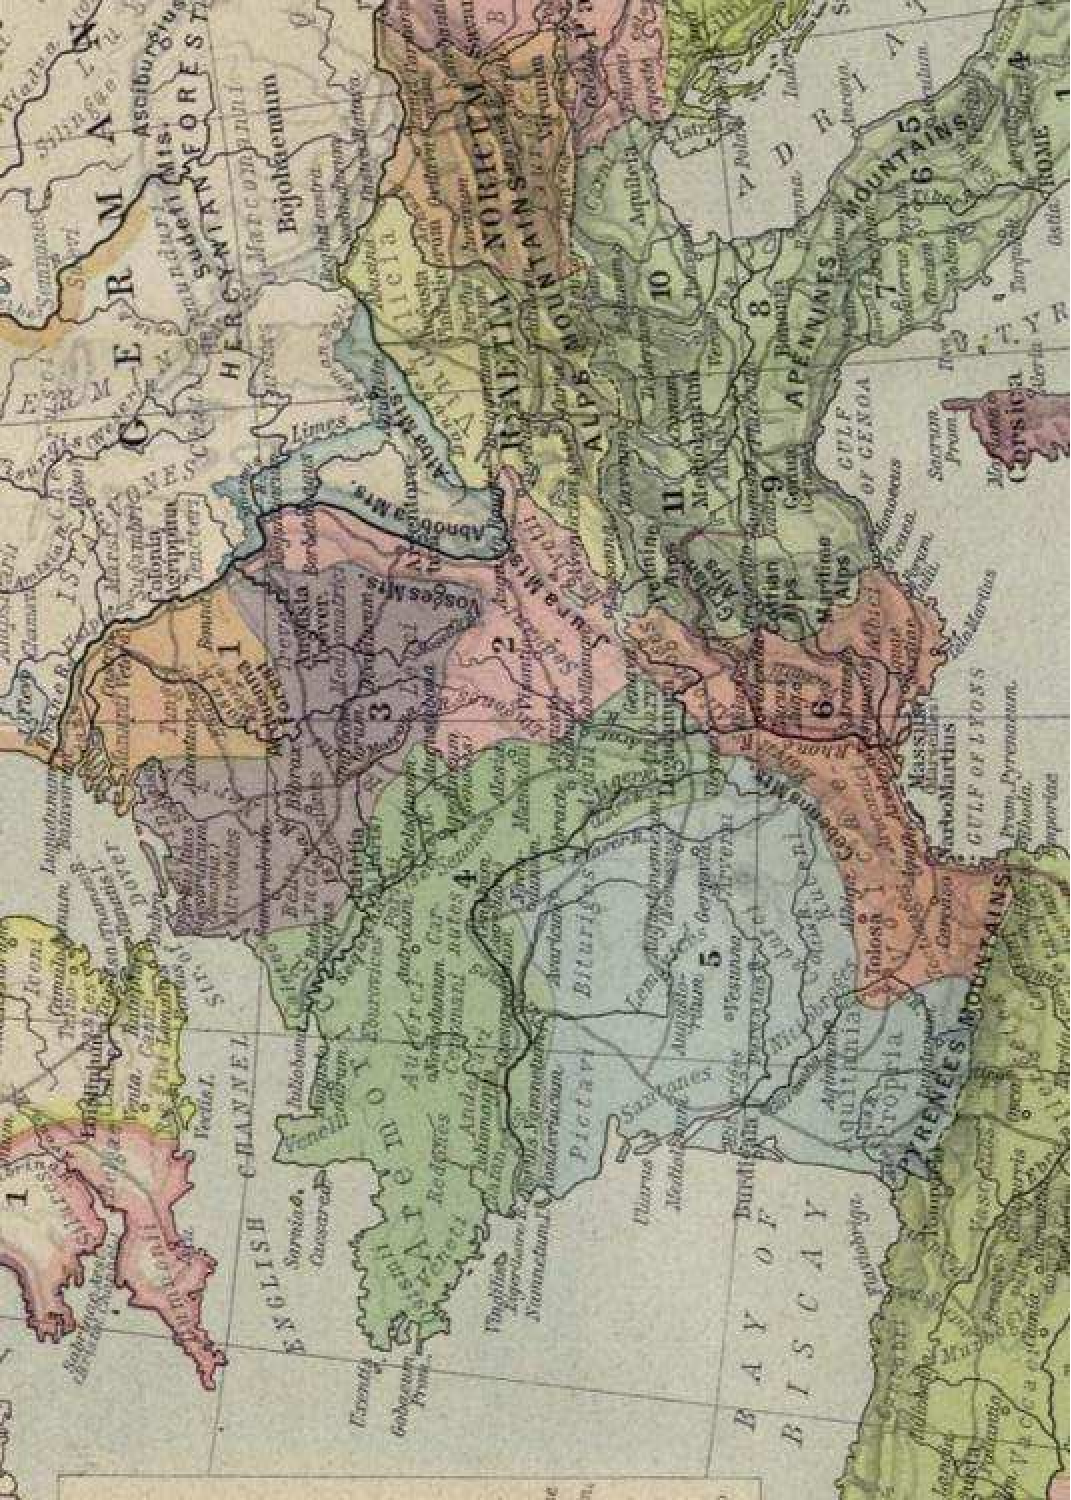
\includegraphics[width=175pt, angle=270]{bilder/Galia}
  \caption{Gallien zur Zeit Caesars}\label{fig_Gallien}
\end{center}
\end{figure}


\begin{table}[htb]
\begin{center}
\begin{tabular}{|l|l|l|}
\hline
Jahr &  Erster Consul & Zweiter Consul\\
\hline \hline
1 & C. Caesar         & L. Aemilius Paullus\\
2 & P. Vinicius       & P. Alfenus Varus\\
3 & L. Aelius Lamia   & M. Servilius\\
4 & Sex. Aelius Catus &  C. Sentius Saturninus\\
5 & L. Valerius Messalla& Cn. Cornelius Cinna \\
suff. & C. Vibius Postumus &  C. Ateius Capito\\
6 & M. Aemilius Lepidus & L. Arruntius\\
\hline
\end{tabular}
 \caption{Römische Konsulen}\label{tab_Konsulen}
\end{center}
\end{table}


\pagebreak

\section{De Bello Hispaniensi}\raggedbottom 

Pharnace superato, Africa recepta, qui ex his proeliis cum
adulescente Cn. Pompeio profugissent, cum . . . et ulterioris
Hispaniae potitus esset, dum Caesar muneribus dandis in Italia
detinetur, . . . quo facilius praesidia contra compararet,
Pompeius in fidem uniuscuiusque civitatis confugere coepit. Ita
partim precibus partim vi bene magna comparata manu provinciam
vastare. Quibus in rebus non nullae civitates sua sponte auxilia
mittebant, item non nullae portas contra cludebant. Ex quibus si
qua oppida vi ceperat, cum aliquis ex ea civitate optime de Cn.
Pompeio meritus civis esset, propter pecuniae magnitudinem alia
qua ei inferebatur causa, ut eo de medio sublato ex eius pecunia
latronum largitio fieret. Ita pacis commoda hoste +hortato+
maiores augebantur copiae. +Hoc crebris nuntiis in Italiam missis
civitates contrariae Pompeio+ auxilia sibi depostulabant.

C. Caesar dictator tertio, designatus dictator quarto multis
+iterante diebus coniectis+ cum celeri festinatione ad bellum
conficiendum in Hispaniam cum venisset, legatique Cordubenses, qui
a Cn. Pompelo discessissent, Caesari obviam venissent, a quibus
nuntiabatur nocturno tempore oppidum Cordubam capi posse, quod nec
opinantibus adversariis eius provinciae potitus esset, simulque
quod tabellariis, qui a Cn. Pompeio dispositi omnibus locis
essent, qui certiorem Cn. Pompeium de Caesaris adventu facerent .
. . multa praeterea veri similia proponebant. Quibus rebus
adductus quos legatos ante exercitui praefecerat Q. Pedium et Q.
Fabium Maximum de suo adventu facit certiores, utque sibi
equitatus qui ex provincia fuisset praesidio esset. Ad quos
celerius quam ipsi opinati sunt appropinquavit neque, ut ipse
voluit, equitatum sibi praesidio habuit.

Erat idem temporis Sex. Pompeius frater qui cum praesidio Cordubam
tenebat, quod eius provinciae caput esse existimabatur; ipse autem
Cn. Pompeius adulescens Uliam oppidum oppugnabat et fere iam
aliquot mensibus ibi detinebatur. Quo ex oppido cognito Caesaris
adventu legati clam praesidia Cn. Pompei Caesarem cum adissent,
petere coeperunt uti sibi primo quoque tempore subsidium mitteret.
Caesar - eam civitatem omni tempore optime de populo Romano
meritam esse - celeriter sex cohortis secunda vigilia iubet
proficisci, pari equites numero. Quibus praefecit hominem eius
provinciae notum et non parum scientem, L. Vibiurn Paciaecum. Qui
cum ad Cn. P praesidia venisset, incidit idem temporis ut
tempestate adversa vehementique vento adflictaretur; aditusque vis
tempestatis ita obscurabat ut vix proximum agnoscere possent.
Cuius incommodum summam utilitatem ipsis praebebat. Ita cum ad eum
locum venerunt, iubet binos equites conscendere, et recta per
adversariorum praesidia ad oppidum contendunt. Mediisque eorum
praesidiis cum essent, cum quaereretur qui essent unus ex nostris
respondit, ut sileat verbum facere: nam id temporis conari ad
murum accedere, ut oppidum capiant; et partim tempestate impediti
vigiles non poterant diligentiam praestare, partim illo responso
deterrebantur. Cum ad portam appropinquassent, signo dato ab
oppidanis sunt reccepti, et pedites dispositi partim ibi
remanserunt, equites clamore facto eruptionem in adversariorum
castra fecerunt.

\pagebreak
\section{Weiteres Kapitel}\raggedbottom 
\subsection{Unterkapitel}
\subsection{Unterkapitel}

%%%%%%%%%%%%%%%%%%%%%%%%%%%%%%%%%%%%%%%%%%%%%%%%%%%%%%%%%%%%%%%%%%%%%%%%
%%%% ENDE TEXTTEIL %%%%%%%%%%%%%%%%%%%%%%%%%%%%%%%%%%%%%%%%%%%%%%%%%%%%%
%%%%%%%%%%%%%%%%%%%%%%%%%%%%%%%%%%%%%%%%%%%%%%%%%%%%%%%%%%%%%%%%%%%%%%%%

\clearpage

% Entfernen Sie das Kommentar aus der nachfolgenden Zeile, falls Sie einen Anhang in der Arbeit verwenden wollen. Beachten Sie, dass Sie sich im Verlauf der Arbeit mit \ref{...} (z.B. \ref{anhang:zusatz1}) auf den Anhang beziehen.
%
% Default to the notebook output style

    


% Inherit from the specified cell style.




    
\documentclass[12pt]{article}

    
    
    \usepackage[T1]{fontenc}
    % Nicer default font (+ math font) than Computer Modern for most use cases
    \usepackage{mathpazo}

    % Basic figure setup, for now with no caption control since it's done
    % automatically by Pandoc (which extracts ![](path) syntax from Markdown).
    \usepackage{graphicx}
    % We will generate all images so they have a width \maxwidth. This means
    % that they will get their normal width if they fit onto the page, but
    % are scaled down if they would overflow the margins.
    \makeatletter
    \def\maxwidth{\ifdim\Gin@nat@width>\linewidth\linewidth
    \else\Gin@nat@width\fi}
    \makeatother
    \let\Oldincludegraphics\includegraphics
    % Set max figure width to be 80% of text width, for now hardcoded.
    \renewcommand{\includegraphics}[1]{\Oldincludegraphics[width=.8\maxwidth]{#1}}
    % Ensure that by default, figures have no caption (until we provide a
    % proper Figure object with a Caption API and a way to capture that
    % in the conversion process - todo).
    \usepackage{caption}
    \DeclareCaptionLabelFormat{nolabel}{}
    \captionsetup{labelformat=nolabel}

    \usepackage{adjustbox} % Used to constrain images to a maximum size 
    \usepackage{xcolor} % Allow colors to be defined
    \usepackage{enumerate} % Needed for markdown enumerations to work
    \usepackage{geometry} % Used to adjust the document margins
    \usepackage{amsmath} % Equations
    \usepackage{amssymb} % Equations
    \usepackage{textcomp} % defines textquotesingle
    % Hack from http://tex.stackexchange.com/a/47451/13684:
    \AtBeginDocument{%
        \def\PYZsq{\textquotesingle}% Upright quotes in Pygmentized code
    }
    \usepackage{upquote} % Upright quotes for verbatim code
    \usepackage{eurosym} % defines \euro
    \usepackage[mathletters]{ucs} % Extended unicode (utf-8) support
    \usepackage[utf8x]{inputenc} % Allow utf-8 characters in the tex document
    \usepackage{fancyvrb} % verbatim replacement that allows latex
    \usepackage{grffile} % extends the file name processing of package graphics 
                         % to support a larger range 
    % The hyperref package gives us a pdf with properly built
    % internal navigation ('pdf bookmarks' for the table of contents,
    % internal cross-reference links, web links for URLs, etc.)
    \usepackage{hyperref}
    \usepackage{longtable} % longtable support required by pandoc >1.10
    \usepackage{booktabs}  % table support for pandoc > 1.12.2
    \usepackage[inline]{enumitem} % IRkernel/repr support (it uses the enumerate* environment)
    \usepackage[normalem]{ulem} % ulem is needed to support strikethroughs (\sout)
                                % normalem makes italics be italics, not underlines
    \usepackage{mathrsfs}
    

    
    
    % Colors for the hyperref package
    \definecolor{urlcolor}{rgb}{0,.145,.698}
    \definecolor{linkcolor}{rgb}{.71,0.21,0.01}
    \definecolor{citecolor}{rgb}{.12,.54,.11}

    % ANSI colors
    \definecolor{ansi-black}{HTML}{3E424D}
    \definecolor{ansi-black-intense}{HTML}{282C36}
    \definecolor{ansi-red}{HTML}{E75C58}
    \definecolor{ansi-red-intense}{HTML}{B22B31}
    \definecolor{ansi-green}{HTML}{00A250}
    \definecolor{ansi-green-intense}{HTML}{007427}
    \definecolor{ansi-yellow}{HTML}{DDB62B}
    \definecolor{ansi-yellow-intense}{HTML}{B27D12}
    \definecolor{ansi-blue}{HTML}{208FFB}
    \definecolor{ansi-blue-intense}{HTML}{0065CA}
    \definecolor{ansi-magenta}{HTML}{D160C4}
    \definecolor{ansi-magenta-intense}{HTML}{A03196}
    \definecolor{ansi-cyan}{HTML}{60C6C8}
    \definecolor{ansi-cyan-intense}{HTML}{258F8F}
    \definecolor{ansi-white}{HTML}{C5C1B4}
    \definecolor{ansi-white-intense}{HTML}{A1A6B2}
    \definecolor{ansi-default-inverse-fg}{HTML}{FFFFFF}
    \definecolor{ansi-default-inverse-bg}{HTML}{000000}

    % commands and environments needed by pandoc snippets
    % extracted from the output of `pandoc -s`
    \providecommand{\tightlist}{%
      \setlength{\itemsep}{0pt}\setlength{\parskip}{0pt}}
    \DefineVerbatimEnvironment{Highlighting}{Verbatim}{commandchars=\\\{\}}
    % Add ',fontsize=\small' for more characters per line
    \newenvironment{Shaded}{}{}
    \newcommand{\KeywordTok}[1]{\textcolor[rgb]{0.00,0.44,0.13}{\textbf{{#1}}}}
    \newcommand{\DataTypeTok}[1]{\textcolor[rgb]{0.56,0.13,0.00}{{#1}}}
    \newcommand{\DecValTok}[1]{\textcolor[rgb]{0.25,0.63,0.44}{{#1}}}
    \newcommand{\BaseNTok}[1]{\textcolor[rgb]{0.25,0.63,0.44}{{#1}}}
    \newcommand{\FloatTok}[1]{\textcolor[rgb]{0.25,0.63,0.44}{{#1}}}
    \newcommand{\CharTok}[1]{\textcolor[rgb]{0.25,0.44,0.63}{{#1}}}
    \newcommand{\StringTok}[1]{\textcolor[rgb]{0.25,0.44,0.63}{{#1}}}
    \newcommand{\CommentTok}[1]{\textcolor[rgb]{0.38,0.63,0.69}{\textit{{#1}}}}
    \newcommand{\OtherTok}[1]{\textcolor[rgb]{0.00,0.44,0.13}{{#1}}}
    \newcommand{\AlertTok}[1]{\textcolor[rgb]{1.00,0.00,0.00}{\textbf{{#1}}}}
    \newcommand{\FunctionTok}[1]{\textcolor[rgb]{0.02,0.16,0.49}{{#1}}}
    \newcommand{\RegionMarkerTok}[1]{{#1}}
    \newcommand{\ErrorTok}[1]{\textcolor[rgb]{1.00,0.00,0.00}{\textbf{{#1}}}}
    \newcommand{\NormalTok}[1]{{#1}}
    
    % Additional commands for more recent versions of Pandoc
    \newcommand{\ConstantTok}[1]{\textcolor[rgb]{0.53,0.00,0.00}{{#1}}}
    \newcommand{\SpecialCharTok}[1]{\textcolor[rgb]{0.25,0.44,0.63}{{#1}}}
    \newcommand{\VerbatimStringTok}[1]{\textcolor[rgb]{0.25,0.44,0.63}{{#1}}}
    \newcommand{\SpecialStringTok}[1]{\textcolor[rgb]{0.73,0.40,0.53}{{#1}}}
    \newcommand{\ImportTok}[1]{{#1}}
    \newcommand{\DocumentationTok}[1]{\textcolor[rgb]{0.73,0.13,0.13}{\textit{{#1}}}}
    \newcommand{\AnnotationTok}[1]{\textcolor[rgb]{0.38,0.63,0.69}{\textbf{\textit{{#1}}}}}
    \newcommand{\CommentVarTok}[1]{\textcolor[rgb]{0.38,0.63,0.69}{\textbf{\textit{{#1}}}}}
    \newcommand{\VariableTok}[1]{\textcolor[rgb]{0.10,0.09,0.49}{{#1}}}
    \newcommand{\ControlFlowTok}[1]{\textcolor[rgb]{0.00,0.44,0.13}{\textbf{{#1}}}}
    \newcommand{\OperatorTok}[1]{\textcolor[rgb]{0.40,0.40,0.40}{{#1}}}
    \newcommand{\BuiltInTok}[1]{{#1}}
    \newcommand{\ExtensionTok}[1]{{#1}}
    \newcommand{\PreprocessorTok}[1]{\textcolor[rgb]{0.74,0.48,0.00}{{#1}}}
    \newcommand{\AttributeTok}[1]{\textcolor[rgb]{0.49,0.56,0.16}{{#1}}}
    \newcommand{\InformationTok}[1]{\textcolor[rgb]{0.38,0.63,0.69}{\textbf{\textit{{#1}}}}}
    \newcommand{\WarningTok}[1]{\textcolor[rgb]{0.38,0.63,0.69}{\textbf{\textit{{#1}}}}}
    
    
    % Define a nice break command that doesn't care if a line doesn't already
    % exist.
    \def\br{\hspace*{\fill} \\* }
    % Math Jax compatibility definitions
    \def\gt{>}
    \def\lt{<}
    \let\Oldtex\TeX
    \let\Oldlatex\LaTeX
    \renewcommand{\TeX}{\textrm{\Oldtex}}
    \renewcommand{\LaTeX}{\textrm{\Oldlatex}}
    % Document parameters
    % Document title
    \title{anhang}
    
    
    
    
    

    % Pygments definitions
    
\makeatletter
\def\PY@reset{\let\PY@it=\relax \let\PY@bf=\relax%
    \let\PY@ul=\relax \let\PY@tc=\relax%
    \let\PY@bc=\relax \let\PY@ff=\relax}
\def\PY@tok#1{\csname PY@tok@#1\endcsname}
\def\PY@toks#1+{\ifx\relax#1\empty\else%
    \PY@tok{#1}\expandafter\PY@toks\fi}
\def\PY@do#1{\PY@bc{\PY@tc{\PY@ul{%
    \PY@it{\PY@bf{\PY@ff{#1}}}}}}}
\def\PY#1#2{\PY@reset\PY@toks#1+\relax+\PY@do{#2}}

\expandafter\def\csname PY@tok@w\endcsname{\def\PY@tc##1{\textcolor[rgb]{0.73,0.73,0.73}{##1}}}
\expandafter\def\csname PY@tok@c\endcsname{\let\PY@it=\textit\def\PY@tc##1{\textcolor[rgb]{0.25,0.50,0.50}{##1}}}
\expandafter\def\csname PY@tok@cp\endcsname{\def\PY@tc##1{\textcolor[rgb]{0.74,0.48,0.00}{##1}}}
\expandafter\def\csname PY@tok@k\endcsname{\let\PY@bf=\textbf\def\PY@tc##1{\textcolor[rgb]{0.00,0.50,0.00}{##1}}}
\expandafter\def\csname PY@tok@kp\endcsname{\def\PY@tc##1{\textcolor[rgb]{0.00,0.50,0.00}{##1}}}
\expandafter\def\csname PY@tok@kt\endcsname{\def\PY@tc##1{\textcolor[rgb]{0.69,0.00,0.25}{##1}}}
\expandafter\def\csname PY@tok@o\endcsname{\def\PY@tc##1{\textcolor[rgb]{0.40,0.40,0.40}{##1}}}
\expandafter\def\csname PY@tok@ow\endcsname{\let\PY@bf=\textbf\def\PY@tc##1{\textcolor[rgb]{0.67,0.13,1.00}{##1}}}
\expandafter\def\csname PY@tok@nb\endcsname{\def\PY@tc##1{\textcolor[rgb]{0.00,0.50,0.00}{##1}}}
\expandafter\def\csname PY@tok@nf\endcsname{\def\PY@tc##1{\textcolor[rgb]{0.00,0.00,1.00}{##1}}}
\expandafter\def\csname PY@tok@nc\endcsname{\let\PY@bf=\textbf\def\PY@tc##1{\textcolor[rgb]{0.00,0.00,1.00}{##1}}}
\expandafter\def\csname PY@tok@nn\endcsname{\let\PY@bf=\textbf\def\PY@tc##1{\textcolor[rgb]{0.00,0.00,1.00}{##1}}}
\expandafter\def\csname PY@tok@ne\endcsname{\let\PY@bf=\textbf\def\PY@tc##1{\textcolor[rgb]{0.82,0.25,0.23}{##1}}}
\expandafter\def\csname PY@tok@nv\endcsname{\def\PY@tc##1{\textcolor[rgb]{0.10,0.09,0.49}{##1}}}
\expandafter\def\csname PY@tok@no\endcsname{\def\PY@tc##1{\textcolor[rgb]{0.53,0.00,0.00}{##1}}}
\expandafter\def\csname PY@tok@nl\endcsname{\def\PY@tc##1{\textcolor[rgb]{0.63,0.63,0.00}{##1}}}
\expandafter\def\csname PY@tok@ni\endcsname{\let\PY@bf=\textbf\def\PY@tc##1{\textcolor[rgb]{0.60,0.60,0.60}{##1}}}
\expandafter\def\csname PY@tok@na\endcsname{\def\PY@tc##1{\textcolor[rgb]{0.49,0.56,0.16}{##1}}}
\expandafter\def\csname PY@tok@nt\endcsname{\let\PY@bf=\textbf\def\PY@tc##1{\textcolor[rgb]{0.00,0.50,0.00}{##1}}}
\expandafter\def\csname PY@tok@nd\endcsname{\def\PY@tc##1{\textcolor[rgb]{0.67,0.13,1.00}{##1}}}
\expandafter\def\csname PY@tok@s\endcsname{\def\PY@tc##1{\textcolor[rgb]{0.73,0.13,0.13}{##1}}}
\expandafter\def\csname PY@tok@sd\endcsname{\let\PY@it=\textit\def\PY@tc##1{\textcolor[rgb]{0.73,0.13,0.13}{##1}}}
\expandafter\def\csname PY@tok@si\endcsname{\let\PY@bf=\textbf\def\PY@tc##1{\textcolor[rgb]{0.73,0.40,0.53}{##1}}}
\expandafter\def\csname PY@tok@se\endcsname{\let\PY@bf=\textbf\def\PY@tc##1{\textcolor[rgb]{0.73,0.40,0.13}{##1}}}
\expandafter\def\csname PY@tok@sr\endcsname{\def\PY@tc##1{\textcolor[rgb]{0.73,0.40,0.53}{##1}}}
\expandafter\def\csname PY@tok@ss\endcsname{\def\PY@tc##1{\textcolor[rgb]{0.10,0.09,0.49}{##1}}}
\expandafter\def\csname PY@tok@sx\endcsname{\def\PY@tc##1{\textcolor[rgb]{0.00,0.50,0.00}{##1}}}
\expandafter\def\csname PY@tok@m\endcsname{\def\PY@tc##1{\textcolor[rgb]{0.40,0.40,0.40}{##1}}}
\expandafter\def\csname PY@tok@gh\endcsname{\let\PY@bf=\textbf\def\PY@tc##1{\textcolor[rgb]{0.00,0.00,0.50}{##1}}}
\expandafter\def\csname PY@tok@gu\endcsname{\let\PY@bf=\textbf\def\PY@tc##1{\textcolor[rgb]{0.50,0.00,0.50}{##1}}}
\expandafter\def\csname PY@tok@gd\endcsname{\def\PY@tc##1{\textcolor[rgb]{0.63,0.00,0.00}{##1}}}
\expandafter\def\csname PY@tok@gi\endcsname{\def\PY@tc##1{\textcolor[rgb]{0.00,0.63,0.00}{##1}}}
\expandafter\def\csname PY@tok@gr\endcsname{\def\PY@tc##1{\textcolor[rgb]{1.00,0.00,0.00}{##1}}}
\expandafter\def\csname PY@tok@ge\endcsname{\let\PY@it=\textit}
\expandafter\def\csname PY@tok@gs\endcsname{\let\PY@bf=\textbf}
\expandafter\def\csname PY@tok@gp\endcsname{\let\PY@bf=\textbf\def\PY@tc##1{\textcolor[rgb]{0.00,0.00,0.50}{##1}}}
\expandafter\def\csname PY@tok@go\endcsname{\def\PY@tc##1{\textcolor[rgb]{0.53,0.53,0.53}{##1}}}
\expandafter\def\csname PY@tok@gt\endcsname{\def\PY@tc##1{\textcolor[rgb]{0.00,0.27,0.87}{##1}}}
\expandafter\def\csname PY@tok@err\endcsname{\def\PY@bc##1{\setlength{\fboxsep}{0pt}\fcolorbox[rgb]{1.00,0.00,0.00}{1,1,1}{\strut ##1}}}
\expandafter\def\csname PY@tok@kc\endcsname{\let\PY@bf=\textbf\def\PY@tc##1{\textcolor[rgb]{0.00,0.50,0.00}{##1}}}
\expandafter\def\csname PY@tok@kd\endcsname{\let\PY@bf=\textbf\def\PY@tc##1{\textcolor[rgb]{0.00,0.50,0.00}{##1}}}
\expandafter\def\csname PY@tok@kn\endcsname{\let\PY@bf=\textbf\def\PY@tc##1{\textcolor[rgb]{0.00,0.50,0.00}{##1}}}
\expandafter\def\csname PY@tok@kr\endcsname{\let\PY@bf=\textbf\def\PY@tc##1{\textcolor[rgb]{0.00,0.50,0.00}{##1}}}
\expandafter\def\csname PY@tok@bp\endcsname{\def\PY@tc##1{\textcolor[rgb]{0.00,0.50,0.00}{##1}}}
\expandafter\def\csname PY@tok@fm\endcsname{\def\PY@tc##1{\textcolor[rgb]{0.00,0.00,1.00}{##1}}}
\expandafter\def\csname PY@tok@vc\endcsname{\def\PY@tc##1{\textcolor[rgb]{0.10,0.09,0.49}{##1}}}
\expandafter\def\csname PY@tok@vg\endcsname{\def\PY@tc##1{\textcolor[rgb]{0.10,0.09,0.49}{##1}}}
\expandafter\def\csname PY@tok@vi\endcsname{\def\PY@tc##1{\textcolor[rgb]{0.10,0.09,0.49}{##1}}}
\expandafter\def\csname PY@tok@vm\endcsname{\def\PY@tc##1{\textcolor[rgb]{0.10,0.09,0.49}{##1}}}
\expandafter\def\csname PY@tok@sa\endcsname{\def\PY@tc##1{\textcolor[rgb]{0.73,0.13,0.13}{##1}}}
\expandafter\def\csname PY@tok@sb\endcsname{\def\PY@tc##1{\textcolor[rgb]{0.73,0.13,0.13}{##1}}}
\expandafter\def\csname PY@tok@sc\endcsname{\def\PY@tc##1{\textcolor[rgb]{0.73,0.13,0.13}{##1}}}
\expandafter\def\csname PY@tok@dl\endcsname{\def\PY@tc##1{\textcolor[rgb]{0.73,0.13,0.13}{##1}}}
\expandafter\def\csname PY@tok@s2\endcsname{\def\PY@tc##1{\textcolor[rgb]{0.73,0.13,0.13}{##1}}}
\expandafter\def\csname PY@tok@sh\endcsname{\def\PY@tc##1{\textcolor[rgb]{0.73,0.13,0.13}{##1}}}
\expandafter\def\csname PY@tok@s1\endcsname{\def\PY@tc##1{\textcolor[rgb]{0.73,0.13,0.13}{##1}}}
\expandafter\def\csname PY@tok@mb\endcsname{\def\PY@tc##1{\textcolor[rgb]{0.40,0.40,0.40}{##1}}}
\expandafter\def\csname PY@tok@mf\endcsname{\def\PY@tc##1{\textcolor[rgb]{0.40,0.40,0.40}{##1}}}
\expandafter\def\csname PY@tok@mh\endcsname{\def\PY@tc##1{\textcolor[rgb]{0.40,0.40,0.40}{##1}}}
\expandafter\def\csname PY@tok@mi\endcsname{\def\PY@tc##1{\textcolor[rgb]{0.40,0.40,0.40}{##1}}}
\expandafter\def\csname PY@tok@il\endcsname{\def\PY@tc##1{\textcolor[rgb]{0.40,0.40,0.40}{##1}}}
\expandafter\def\csname PY@tok@mo\endcsname{\def\PY@tc##1{\textcolor[rgb]{0.40,0.40,0.40}{##1}}}
\expandafter\def\csname PY@tok@ch\endcsname{\let\PY@it=\textit\def\PY@tc##1{\textcolor[rgb]{0.25,0.50,0.50}{##1}}}
\expandafter\def\csname PY@tok@cm\endcsname{\let\PY@it=\textit\def\PY@tc##1{\textcolor[rgb]{0.25,0.50,0.50}{##1}}}
\expandafter\def\csname PY@tok@cpf\endcsname{\let\PY@it=\textit\def\PY@tc##1{\textcolor[rgb]{0.25,0.50,0.50}{##1}}}
\expandafter\def\csname PY@tok@c1\endcsname{\let\PY@it=\textit\def\PY@tc##1{\textcolor[rgb]{0.25,0.50,0.50}{##1}}}
\expandafter\def\csname PY@tok@cs\endcsname{\let\PY@it=\textit\def\PY@tc##1{\textcolor[rgb]{0.25,0.50,0.50}{##1}}}

\def\PYZbs{\char`\\}
\def\PYZus{\char`\_}
\def\PYZob{\char`\{}
\def\PYZcb{\char`\}}
\def\PYZca{\char`\^}
\def\PYZam{\char`\&}
\def\PYZlt{\char`\<}
\def\PYZgt{\char`\>}
\def\PYZsh{\char`\#}
\def\PYZpc{\char`\%}
\def\PYZdl{\char`\$}
\def\PYZhy{\char`\-}
\def\PYZsq{\char`\'}
\def\PYZdq{\char`\"}
\def\PYZti{\char`\~}
% for compatibility with earlier versions
\def\PYZat{@}
\def\PYZlb{[}
\def\PYZrb{]}
\makeatother


    % Exact colors from NB
    \definecolor{incolor}{rgb}{0.0, 0.0, 0.5}
    \definecolor{outcolor}{rgb}{0.545, 0.0, 0.0}



    
    % Prevent overflowing lines due to hard-to-break entities
    \sloppy 
    % Setup hyperref package
    \hypersetup{
      breaklinks=true,  % so long urls are correctly broken across lines
      colorlinks=true,
      urlcolor=urlcolor,
      linkcolor=linkcolor,
      citecolor=citecolor,
      }
    % Slightly bigger margins than the latex defaults
    
    \geometry{verbose,tmargin=0in,bmargin=0in,lmargin=0in,rmargin=0in}
    
    

    \begin{document}
    
    
    %\maketitle
    
    

    
    \begin{Verbatim}[commandchars=\\\{\}]
{\color{incolor}In [{\color{incolor}1}]:} \PY{k+kn}{from} \PY{n+nn}{\PYZus{}fcm} \PY{k}{import} \PY{n}{cmeans}
        \PY{k+kn}{from} \PY{n+nn}{\PYZus{}pfcm} \PY{k}{import} \PY{n}{pfcm}
        \PY{k+kn}{import} \PY{n+nn}{numpy} \PY{k}{as} \PY{n+nn}{np}
        \PY{k+kn}{from} \PY{n+nn}{matplotlib} \PY{k}{import} \PY{n}{pyplot} \PY{k}{as} \PY{n}{plt}
        \PY{k+kn}{import} \PY{n+nn}{csv}
        \PY{k+kn}{from} \PY{n+nn}{mpl\PYZus{}toolkits}\PY{n+nn}{.}\PY{n+nn}{mplot3d} \PY{k}{import} \PY{n}{Axes3D}
        \PY{k+kn}{import} \PY{n+nn}{scipy}\PY{n+nn}{.}\PY{n+nn}{spatial} \PY{k}{as} \PY{n+nn}{spat}
        \PY{k+kn}{import} \PY{n+nn}{itertools}
        \PY{k+kn}{import} \PY{n+nn}{imageio}
        \PY{k+kn}{import} \PY{n+nn}{PIL}
        \PY{k+kn}{import} \PY{n+nn}{math} \PY{k}{as} \PY{n+nn}{mat}
\end{Verbatim}

    \begin{Verbatim}[commandchars=\\\{\}]
{\color{incolor}In [{\color{incolor}2}]:} \PY{c+c1}{\PYZsh{}\PYZsh{}\PYZsh{}\PYZsh{}\PYZsh{}\PYZsh{}\PYZsh{}\PYZsh{}\PYZsh{}\PYZsh{}\PYZsh{}\PYZsh{}\PYZsh{}\PYZsh{}\PYZsh{}\PYZsh{}\PYZsh{}\PYZsh{}\PYZsh{}\PYZsh{}\PYZsh{}\PYZsh{}\PYZsh{}\PYZsh{}\PYZsh{}\PYZsh{}\PYZsh{}\PYZsh{}\PYZsh{}\PYZsh{}\PYZsh{}\PYZsh{}\PYZsh{}\PYZsh{}\PYZsh{}\PYZsh{}\PYZsh{}\PYZsh{}\PYZsh{}\PYZsh{}\PYZsh{}\PYZsh{}\PYZsh{}\PYZsh{}\PYZsh{}\PYZsh{}\PYZsh{}\PYZsh{}\PYZsh{}\PYZsh{}\PYZsh{}\PYZsh{}\PYZsh{}\PYZsh{}\PYZsh{}\PYZsh{}\PYZsh{}\PYZsh{}\PYZsh{}\PYZsh{}\PYZsh{}\PYZsh{}\PYZsh{}\PYZsh{}\PYZsh{}\PYZsh{}\PYZsh{}\PYZsh{}\PYZsh{}\PYZsh{}\PYZsh{}\PYZsh{}\PYZsh{}\PYZsh{}\PYZsh{}\PYZsh{}\PYZsh{}\PYZsh{}\PYZsh{}\PYZsh{}\PYZsh{}\PYZsh{}\PYZsh{}\PYZsh{}\PYZsh{}\PYZsh{}\PYZsh{}\PYZsh{}\PYZsh{}}
        \PY{c+c1}{\PYZsh{}\PYZsh{}\PYZsh{}\PYZsh{}\PYZsh{}\PYZsh{}\PYZsh{}\PYZsh{}\PYZsh{}\PYZsh{}\PYZsh{}\PYZsh{}\PYZsh{} Geodatensatz mit vielen Punkten, aber wenigen Dimensionen \PYZsh{}\PYZsh{}\PYZsh{}\PYZsh{}\PYZsh{}\PYZsh{}\PYZsh{}\PYZsh{}\PYZsh{}\PYZsh{}\PYZsh{}\PYZsh{}\PYZsh{}\PYZsh{}\PYZsh{}\PYZsh{}\PYZsh{}}
        \PY{c+c1}{\PYZsh{}\PYZsh{}\PYZsh{}\PYZsh{}\PYZsh{}\PYZsh{}\PYZsh{}\PYZsh{}\PYZsh{}\PYZsh{}\PYZsh{}\PYZsh{}\PYZsh{}         http://download.geonames.org/export/zip/          \PYZsh{}\PYZsh{}\PYZsh{}\PYZsh{}\PYZsh{}\PYZsh{}\PYZsh{}\PYZsh{}\PYZsh{}\PYZsh{}\PYZsh{}\PYZsh{}\PYZsh{}\PYZsh{}\PYZsh{}\PYZsh{}\PYZsh{}}
        \PY{c+c1}{\PYZsh{}\PYZsh{}\PYZsh{}\PYZsh{}\PYZsh{}\PYZsh{}\PYZsh{}\PYZsh{}\PYZsh{}\PYZsh{}\PYZsh{}\PYZsh{}\PYZsh{}\PYZsh{}\PYZsh{}\PYZsh{}\PYZsh{}\PYZsh{}\PYZsh{}\PYZsh{}\PYZsh{}\PYZsh{}\PYZsh{}\PYZsh{}\PYZsh{}\PYZsh{}\PYZsh{}\PYZsh{}\PYZsh{}\PYZsh{}\PYZsh{}\PYZsh{}\PYZsh{}\PYZsh{}\PYZsh{}\PYZsh{}\PYZsh{}\PYZsh{}\PYZsh{}\PYZsh{}\PYZsh{}\PYZsh{}\PYZsh{}\PYZsh{}\PYZsh{}\PYZsh{}\PYZsh{}\PYZsh{}\PYZsh{}\PYZsh{}\PYZsh{}\PYZsh{}\PYZsh{}\PYZsh{}\PYZsh{}\PYZsh{}\PYZsh{}\PYZsh{}\PYZsh{}\PYZsh{}\PYZsh{}\PYZsh{}\PYZsh{}\PYZsh{}\PYZsh{}\PYZsh{}\PYZsh{}\PYZsh{}\PYZsh{}\PYZsh{}\PYZsh{}\PYZsh{}\PYZsh{}\PYZsh{}\PYZsh{}\PYZsh{}\PYZsh{}\PYZsh{}\PYZsh{}\PYZsh{}\PYZsh{}\PYZsh{}\PYZsh{}\PYZsh{}\PYZsh{}\PYZsh{}\PYZsh{}\PYZsh{}\PYZsh{}}
        
        \PY{n}{text\PYZus{}file} \PY{o}{=} \PY{n+nb}{open}\PY{p}{(}\PY{l+s+s2}{\PYZdq{}}\PY{l+s+s2}{allCountries.txt}\PY{l+s+s2}{\PYZdq{}}\PY{p}{,} \PY{l+s+s2}{\PYZdq{}}\PY{l+s+s2}{r}\PY{l+s+s2}{\PYZdq{}}\PY{p}{,} \PY{n}{encoding}\PY{o}{=}\PY{l+s+s2}{\PYZdq{}}\PY{l+s+s2}{utf8}\PY{l+s+s2}{\PYZdq{}}\PY{p}{)}
        \PY{n}{ac\PYZus{}lines} \PY{o}{=} \PY{n}{text\PYZus{}file}\PY{o}{.}\PY{n}{read}\PY{p}{(}\PY{p}{)}\PY{o}{.}\PY{n}{split}\PY{p}{(}\PY{l+s+s1}{\PYZsq{}}\PY{l+s+se}{\PYZbs{}n}\PY{l+s+s1}{\PYZsq{}}\PY{p}{)}
        \PY{n}{text\PYZus{}file}\PY{o}{.}\PY{n}{close}\PY{p}{(}\PY{p}{)}
        \PY{n}{geonames} \PY{o}{=} \PY{n}{np}\PY{o}{.}\PY{n}{empty}\PY{p}{(}\PY{p}{[}\PY{n}{np}\PY{o}{.}\PY{n}{size}\PY{p}{(}\PY{n}{ac\PYZus{}lines}\PY{p}{)}\PY{o}{\PYZhy{}}\PY{l+m+mi}{1}\PY{p}{,}\PY{n}{np}\PY{o}{.}\PY{n}{size}\PY{p}{(}\PY{n}{ac\PYZus{}lines}\PY{p}{[}\PY{l+m+mi}{0}\PY{p}{]}\PY{o}{.}\PY{n}{split}\PY{p}{(}\PY{l+s+s1}{\PYZsq{}}\PY{l+s+se}{\PYZbs{}t}\PY{l+s+s1}{\PYZsq{}}\PY{p}{)}\PY{p}{)}\PY{p}{]}\PY{p}{,}\PY{n}{dtype}\PY{o}{=}\PY{n+nb}{object}\PY{p}{)}
        \PY{k}{for} \PY{n}{i} \PY{o+ow}{in} \PY{n+nb}{range}\PY{p}{(}\PY{l+m+mi}{0}\PY{p}{,}\PY{n}{np}\PY{o}{.}\PY{n}{size}\PY{p}{(}\PY{n}{ac\PYZus{}lines}\PY{p}{)}\PY{o}{\PYZhy{}}\PY{l+m+mi}{1}\PY{p}{)}\PY{p}{:}
            \PY{n}{geonames}\PY{p}{[}\PY{n}{i}\PY{p}{]} \PY{o}{=} \PY{n}{ac\PYZus{}lines}\PY{p}{[}\PY{n}{i}\PY{p}{]}\PY{o}{.}\PY{n}{split}\PY{p}{(}\PY{l+s+s1}{\PYZsq{}}\PY{l+s+se}{\PYZbs{}t}\PY{l+s+s1}{\PYZsq{}}\PY{p}{)}
        \PY{n+nb}{print}\PY{p}{(}\PY{l+s+s2}{\PYZdq{}}\PY{l+s+s2}{Dieser Datensatz hat }\PY{l+s+s2}{\PYZdq{}}\PY{o}{+}\PY{n+nb}{str}\PY{p}{(}\PY{n}{geonames}\PY{o}{.}\PY{n}{shape}\PY{p}{[}\PY{l+m+mi}{0}\PY{p}{]}\PY{p}{)}\PY{o}{+}\PY{l+s+s2}{\PYZdq{}}\PY{l+s+s2}{ Datenpunkte und }\PY{l+s+s2}{\PYZdq{}}
                                         \PY{o}{+}\PY{n+nb}{str}\PY{p}{(}\PY{n}{geonames}\PY{o}{.}\PY{n}{shape}\PY{p}{[}\PY{l+m+mi}{1}\PY{p}{]}\PY{p}{)}\PY{o}{+}\PY{l+s+s2}{\PYZdq{}}\PY{l+s+s2}{ Attribute.}\PY{l+s+s2}{\PYZdq{}}\PY{p}{)}
\end{Verbatim}

    \begin{Verbatim}[commandchars=\\\{\}]
Dieser Datensatz hat 1264940 Datenpunkte und 12 Attribute.

    \end{Verbatim}

    \begin{Verbatim}[commandchars=\\\{\}]
{\color{incolor}In [{\color{incolor}3}]:} \PY{c+c1}{\PYZsh{}Visualisierung aller Punkte als \PYZdq{}Landkarte\PYZdq{} mittels pyplot:}
        \PY{n}{worldplot} \PY{o}{=} \PY{n}{plt}\PY{o}{.}\PY{n}{plot}\PY{p}{(}\PY{n}{geonames}\PY{p}{[}\PY{l+m+mi}{0}\PY{p}{:}\PY{p}{,}\PY{l+m+mi}{10}\PY{p}{]}\PY{o}{.}\PY{n}{astype}\PY{p}{(}\PY{n+nb}{float}\PY{p}{)}\PY{p}{,} \PY{n}{geonames}\PY{p}{[}\PY{l+m+mi}{0}\PY{p}{:}\PY{p}{,}\PY{l+m+mi}{9}\PY{p}{]}\PY{o}{.}\PY{n}{astype}\PY{p}{(}\PY{n+nb}{float}\PY{p}{)}\PY{p}{,} \PY{l+s+s1}{\PYZsq{}}\PY{l+s+s1}{g.}\PY{l+s+s1}{\PYZsq{}}\PY{p}{)}
        \PY{n}{plt}\PY{o}{.}\PY{n}{setp}\PY{p}{(}\PY{n}{worldplot}\PY{p}{,} \PY{n}{markersize}\PY{o}{=}\PY{l+m+mf}{0.2}\PY{p}{)}
        \PY{n}{plt}\PY{o}{.}\PY{n}{show}\PY{p}{(}\PY{p}{)}
\end{Verbatim}

    \begin{center}
    \adjustimage{max size={0.9\linewidth}{0.9\paperheight}}{output_2_0.png}
    \end{center}
    { \hspace*{\fill} \\}
    
    \begin{Verbatim}[commandchars=\\\{\}]
{\color{incolor}In [{\color{incolor}4}]:} \PY{c+c1}{\PYZsh{}Ausschnitt der Landkarte (hier Europa) betrachten:}
        \PY{n}{breitengrad} \PY{o}{=} \PY{n}{geonames}\PY{p}{[}\PY{l+m+mi}{0}\PY{p}{:}\PY{p}{,}\PY{l+m+mi}{9}\PY{p}{]}\PY{o}{.}\PY{n}{astype}\PY{p}{(}\PY{n+nb}{float}\PY{p}{)}
        \PY{n}{laengengrad} \PY{o}{=} \PY{n}{geonames}\PY{p}{[}\PY{l+m+mi}{0}\PY{p}{:}\PY{p}{,}\PY{l+m+mi}{10}\PY{p}{]}\PY{o}{.}\PY{n}{astype}\PY{p}{(}\PY{n+nb}{float}\PY{p}{)}
        \PY{n}{condition} \PY{o}{=} \PY{p}{[}\PY{p}{(}\PY{n}{breitengrad}\PY{o}{\PYZgt{}}\PY{l+m+mi}{30}\PY{p}{)} \PY{o}{\PYZam{}} \PY{p}{(}\PY{n}{breitengrad} \PY{o}{\PYZlt{}}\PY{l+m+mi}{70}\PY{p}{)} 
                     \PY{o}{\PYZam{}} \PY{p}{(}\PY{n}{laengengrad}\PY{o}{\PYZgt{}}\PY{o}{\PYZhy{}}\PY{l+m+mi}{10}\PY{p}{)} \PY{o}{\PYZam{}} \PY{p}{(}\PY{n}{laengengrad} \PY{o}{\PYZlt{}}\PY{l+m+mi}{50}\PY{p}{)}\PY{p}{]}
        \PY{n}{cond\PYZus{}a} \PY{o}{=} \PY{n}{np}\PY{o}{.}\PY{n}{extract}\PY{p}{(}\PY{n}{condition}\PY{p}{,} \PY{n}{breitengrad}\PY{p}{)}
        \PY{n}{cond\PYZus{}b} \PY{o}{=} \PY{n}{np}\PY{o}{.}\PY{n}{extract}\PY{p}{(}\PY{n}{condition}\PY{p}{,} \PY{n}{laengengrad}\PY{p}{)}
        \PY{n}{euplot} \PY{o}{=} \PY{n}{plt}\PY{o}{.}\PY{n}{plot}\PY{p}{(}\PY{n}{cond\PYZus{}b}\PY{p}{,}\PY{n}{cond\PYZus{}a}\PY{p}{,} \PY{l+s+s1}{\PYZsq{}}\PY{l+s+s1}{g.}\PY{l+s+s1}{\PYZsq{}}\PY{p}{)}
        \PY{n}{plt}\PY{o}{.}\PY{n}{setp}\PY{p}{(}\PY{n}{euplot}\PY{p}{,} \PY{n}{markersize}\PY{o}{=}\PY{l+m+mf}{0.5}\PY{p}{)}
        \PY{n}{plt}\PY{o}{.}\PY{n}{show}\PY{p}{(}\PY{p}{)}
\end{Verbatim}

    \begin{center}
    \adjustimage{max size={0.9\linewidth}{0.9\paperheight}}{output_3_0.png}
    \end{center}
    { \hspace*{\fill} \\}
\newpage    
    \begin{Verbatim}[commandchars=\\\{\}]
{\color{incolor}In [{\color{incolor}5}]:} \PY{c+c1}{\PYZsh{}\PYZsh{}\PYZsh{}\PYZsh{}\PYZsh{}\PYZsh{}\PYZsh{}\PYZsh{}\PYZsh{}\PYZsh{}\PYZsh{}\PYZsh{}\PYZsh{}\PYZsh{}\PYZsh{}\PYZsh{}\PYZsh{}\PYZsh{}\PYZsh{}\PYZsh{}\PYZsh{}\PYZsh{}\PYZsh{}\PYZsh{}\PYZsh{}\PYZsh{}\PYZsh{}\PYZsh{}\PYZsh{}\PYZsh{}\PYZsh{}\PYZsh{}\PYZsh{}\PYZsh{}\PYZsh{}\PYZsh{}\PYZsh{}\PYZsh{}\PYZsh{}\PYZsh{}\PYZsh{}\PYZsh{}\PYZsh{}\PYZsh{}\PYZsh{}\PYZsh{}\PYZsh{}\PYZsh{}\PYZsh{}\PYZsh{}\PYZsh{}\PYZsh{}\PYZsh{}\PYZsh{}\PYZsh{}\PYZsh{}\PYZsh{}\PYZsh{}\PYZsh{}\PYZsh{}\PYZsh{}\PYZsh{}\PYZsh{}\PYZsh{}\PYZsh{}\PYZsh{}\PYZsh{}\PYZsh{}\PYZsh{}\PYZsh{}\PYZsh{}\PYZsh{}\PYZsh{}\PYZsh{}\PYZsh{}\PYZsh{}\PYZsh{}\PYZsh{}\PYZsh{}\PYZsh{}\PYZsh{}\PYZsh{}\PYZsh{}\PYZsh{}\PYZsh{}\PYZsh{}\PYZsh{}\PYZsh{}\PYZsh{}}
        \PY{c+c1}{\PYZsh{}\PYZsh{}\PYZsh{}\PYZsh{}\PYZsh{}\PYZsh{}\PYZsh{}\PYZsh{}\PYZsh{}\PYZsh{}\PYZsh{}\PYZsh{}\PYZsh{}             Hochdimensionaler Geodatensatz                  \PYZsh{}\PYZsh{}\PYZsh{}\PYZsh{}\PYZsh{}\PYZsh{}\PYZsh{}\PYZsh{}\PYZsh{}\PYZsh{}\PYZsh{}\PYZsh{}\PYZsh{}\PYZsh{}\PYZsh{}}
        \PY{c+c1}{\PYZsh{}\PYZsh{}\PYZsh{}\PYZsh{}\PYZsh{}\PYZsh{}\PYZsh{}\PYZsh{}\PYZsh{}\PYZsh{}\PYZsh{}\PYZsh{}\PYZsh{}   https://www.kaggle.com/reubencpereira/spatial\PYZhy{}data\PYZhy{}repo   \PYZsh{}\PYZsh{}\PYZsh{}\PYZsh{}\PYZsh{}\PYZsh{}\PYZsh{}\PYZsh{}\PYZsh{}\PYZsh{}\PYZsh{}\PYZsh{}\PYZsh{}\PYZsh{}\PYZsh{}}
        \PY{c+c1}{\PYZsh{}\PYZsh{}\PYZsh{}\PYZsh{}\PYZsh{}\PYZsh{}\PYZsh{}\PYZsh{}\PYZsh{}\PYZsh{}\PYZsh{}\PYZsh{}\PYZsh{}\PYZsh{}\PYZsh{}\PYZsh{}\PYZsh{}\PYZsh{}\PYZsh{}\PYZsh{}\PYZsh{}\PYZsh{}\PYZsh{}\PYZsh{}\PYZsh{}\PYZsh{}\PYZsh{}\PYZsh{}\PYZsh{}\PYZsh{}\PYZsh{}\PYZsh{}\PYZsh{}\PYZsh{}\PYZsh{}\PYZsh{}\PYZsh{}\PYZsh{}\PYZsh{}\PYZsh{}\PYZsh{}\PYZsh{}\PYZsh{}\PYZsh{}\PYZsh{}\PYZsh{}\PYZsh{}\PYZsh{}\PYZsh{}\PYZsh{}\PYZsh{}\PYZsh{}\PYZsh{}\PYZsh{}\PYZsh{}\PYZsh{}\PYZsh{}\PYZsh{}\PYZsh{}\PYZsh{}\PYZsh{}\PYZsh{}\PYZsh{}\PYZsh{}\PYZsh{}\PYZsh{}\PYZsh{}\PYZsh{}\PYZsh{}\PYZsh{}\PYZsh{}\PYZsh{}\PYZsh{}\PYZsh{}\PYZsh{}\PYZsh{}\PYZsh{}\PYZsh{}\PYZsh{}\PYZsh{}\PYZsh{}\PYZsh{}\PYZsh{}\PYZsh{}\PYZsh{}\PYZsh{}\PYZsh{}\PYZsh{}\PYZsh{}}
\end{Verbatim}

    \begin{Verbatim}[commandchars=\\\{\}]
{\color{incolor}In [{\color{incolor}6}]:} \PY{k}{def} \PY{n+nf}{isFloatable}\PY{p}{(}\PY{n}{value}\PY{p}{)}\PY{p}{:}
            \PY{l+s+sd}{\PYZdq{}\PYZdq{}\PYZdq{}}
        \PY{l+s+sd}{    Überprüft, ob ein gegebener Wert in Typ \PYZdq{}float\PYZdq{} umgewandelt werden kann.}
        \PY{l+s+sd}{    value: zu überprüfender Wert}
        \PY{l+s+sd}{    \PYZdq{}\PYZdq{}\PYZdq{}}
            \PY{k}{try}\PY{p}{:}
                \PY{n+nb}{float}\PY{p}{(}\PY{n}{value}\PY{p}{)}
                \PY{k}{return} \PY{k+kc}{True}
            \PY{k}{except} \PY{n+ne}{ValueError}\PY{p}{:}
                \PY{k}{return} \PY{k+kc}{False}
\end{Verbatim}

    \begin{Verbatim}[commandchars=\\\{\}]
{\color{incolor}In [{\color{incolor}7}]:} \PY{k}{def} \PY{n+nf}{readKivaDataset}\PY{p}{(}\PY{p}{)}\PY{p}{:}
            \PY{l+s+sd}{\PYZdq{}\PYZdq{}\PYZdq{}}
        \PY{l+s+sd}{    Spatial Data Repository auslesen und vorbereiten für Plots. }
        \PY{l+s+sd}{    Gibt außerdem aus, welche Daten in welcher Spalte stehen.}
        \PY{l+s+sd}{    kivaArray: gefilterter Datensatz}
        \PY{l+s+sd}{    \PYZdq{}\PYZdq{}\PYZdq{}}
            \PY{n}{text\PYZus{}file} \PY{o}{=} \PY{n+nb}{open}\PY{p}{(}\PY{l+s+s2}{\PYZdq{}}\PY{l+s+s2}{kivaData\PYZus{}augmented.txt}\PY{l+s+s2}{\PYZdq{}}\PY{p}{,} \PY{l+s+s2}{\PYZdq{}}\PY{l+s+s2}{r}\PY{l+s+s2}{\PYZdq{}}\PY{p}{,} \PY{n}{encoding}\PY{o}{=}\PY{l+s+s2}{\PYZdq{}}\PY{l+s+s2}{utf8}\PY{l+s+s2}{\PYZdq{}}\PY{p}{)}
            \PY{n}{lines} \PY{o}{=} \PY{n}{text\PYZus{}file}\PY{o}{.}\PY{n}{read}\PY{p}{(}\PY{p}{)}\PY{o}{.}\PY{n}{split}\PY{p}{(}\PY{l+s+s1}{\PYZsq{}}\PY{l+s+se}{\PYZbs{}n}\PY{l+s+s1}{\PYZsq{}}\PY{p}{)}
            \PY{n}{text\PYZus{}file}\PY{o}{.}\PY{n}{close}\PY{p}{(}\PY{p}{)}
            \PY{n}{kivaList} \PY{o}{=} \PY{p}{[}\PY{p}{]}
            \PY{k}{for} \PY{n}{l} \PY{o+ow}{in}  \PY{n}{csv}\PY{o}{.}\PY{n}{reader}\PY{p}{(}\PY{n}{lines}\PY{p}{,} \PY{n}{quotechar}\PY{o}{=}\PY{l+s+s1}{\PYZsq{}}\PY{l+s+s1}{\PYZdq{}}\PY{l+s+s1}{\PYZsq{}}\PY{p}{,} \PY{n}{delimiter}\PY{o}{=}\PY{l+s+s1}{\PYZsq{}}\PY{l+s+s1}{,}\PY{l+s+s1}{\PYZsq{}}\PY{p}{,}
                                 \PY{n}{quoting}\PY{o}{=}\PY{n}{csv}\PY{o}{.}\PY{n}{QUOTE\PYZus{}ALL}\PY{p}{,} \PY{n}{skipinitialspace}\PY{o}{=}\PY{k+kc}{True}\PY{p}{)}\PY{p}{:}
                \PY{k}{if}\PY{p}{(}\PY{n+nb}{len}\PY{p}{(}\PY{n}{l}\PY{p}{)}\PY{o}{\PYZgt{}}\PY{l+m+mi}{2}\PY{p}{)}\PY{p}{:}
                    \PY{c+c1}{\PYZsh{}Filter für nicht vorhandene Werte}
                    \PY{k}{if}\PY{p}{(}\PY{c+c1}{\PYZsh{}isFloatable((l[2])    \PYZsh{}Breitengrade}
                       \PY{c+c1}{\PYZsh{}\PYZam{} isFloatable((l[3])  \PYZsh{}Längengrade}
                      \PY{c+c1}{\PYZsh{} \PYZam{} isFloatable((l[30]) \PYZsh{}Höhenwerte}
                      \PY{c+c1}{\PYZsh{} \PYZam{} isFloatable((l[27]) \PYZsh{}Reisezeit bis zur nächsten Großstadt in Std.}
                      \PY{c+c1}{\PYZsh{} \PYZam{} isFloatable((l[28]) \PYZsh{}Durchschnittl. nächtliche Beleuchtungszeit}
                      \PY{c+c1}{\PYZsh{} \PYZam{} isFloatable((l[25]) \PYZsh{}Populationsdichte (Bewohner pro m²)}
                         \PY{n}{isFloatable}\PY{p}{(}\PY{p}{(}\PY{n}{l}\PY{p}{[}\PY{l+m+mi}{26}\PY{p}{]}\PY{p}{)}\PY{p}{)} \PY{c+c1}{\PYZsh{}Niederschlag}
                       \PY{o}{\PYZam{}} \PY{n}{isFloatable}\PY{p}{(}\PY{p}{(}\PY{n}{l}\PY{p}{[}\PY{l+m+mi}{29}\PY{p}{]}\PY{p}{)}\PY{p}{)} \PY{c+c1}{\PYZsh{}Landnutzungsklassifikator}
                       \PY{o}{\PYZam{}} \PY{n}{isFloatable}\PY{p}{(}\PY{p}{(}\PY{n}{l}\PY{p}{[}\PY{l+m+mi}{31}\PY{p}{]}\PY{p}{)}\PY{p}{)}\PY{p}{)}\PY{p}{:} \PY{c+c1}{\PYZsh{}Temperatur                       }
                        \PY{n}{kivaList}\PY{o}{.}\PY{n}{append}\PY{p}{(}\PY{n}{l}\PY{p}{)}
                    \PY{k}{elif}\PY{p}{(}\PY{n}{l}\PY{p}{[}\PY{l+m+mi}{0}\PY{p}{]}\PY{o}{==}\PY{l+s+s2}{\PYZdq{}}\PY{l+s+s2}{region}\PY{l+s+s2}{\PYZdq{}}\PY{p}{)}\PY{p}{:}
                        \PY{n}{kivaList}\PY{o}{.}\PY{n}{append}\PY{p}{(}\PY{n}{l}\PY{p}{)}
            \PY{c+c1}{\PYZsh{}In numpy\PYZhy{}Array umwandeln und die Legende entfernen:}
            \PY{n}{kivaArray} \PY{o}{=} \PY{n}{np}\PY{o}{.}\PY{n}{empty}\PY{p}{(}\PY{p}{[}\PY{n+nb}{len}\PY{p}{(}\PY{n}{kivaList}\PY{p}{)}\PY{o}{\PYZhy{}}\PY{l+m+mi}{1}\PY{p}{,}\PY{n+nb}{len}\PY{p}{(}\PY{n}{kivaList}\PY{p}{[}\PY{l+m+mi}{0}\PY{p}{]}\PY{p}{)}\PY{p}{]}\PY{p}{,}\PY{n}{dtype}\PY{o}{=}\PY{n+nb}{object}\PY{p}{)}
            \PY{k}{for} \PY{n}{l} \PY{o+ow}{in} \PY{n+nb}{range}\PY{p}{(}\PY{l+m+mi}{1}\PY{p}{,}\PY{n+nb}{len}\PY{p}{(}\PY{n}{kivaList}\PY{p}{)}\PY{p}{)}\PY{p}{:}
                    \PY{n}{kivaArray} \PY{p}{[}\PY{n}{l}\PY{o}{\PYZhy{}}\PY{l+m+mi}{1}\PY{p}{]} \PY{o}{=} \PY{n}{kivaList} \PY{p}{[}\PY{n}{l}\PY{p}{]}
            \PY{c+c1}{\PYZsh{}Ausgabe der Attributbeschreibungen je Index:}
            \PY{k}{for} \PY{n}{i} \PY{o+ow}{in} \PY{n+nb}{range}\PY{p}{(}\PY{l+m+mi}{0}\PY{p}{,}\PY{l+m+mi}{43}\PY{p}{)}\PY{p}{:}
                \PY{n+nb}{print}\PY{p}{(}\PY{l+s+s2}{\PYZdq{}}\PY{l+s+s2}{Index }\PY{l+s+s2}{\PYZdq{}}\PY{o}{+}\PY{n+nb}{str}\PY{p}{(}\PY{n}{i}\PY{p}{)}\PY{o}{+}\PY{l+s+s2}{\PYZdq{}}\PY{l+s+s2}{: }\PY{l+s+s2}{\PYZdq{}}\PY{o}{+}\PY{n+nb}{str}\PY{p}{(}\PY{n}{kivaList}\PY{p}{[}\PY{l+m+mi}{0}\PY{p}{]}\PY{p}{[}\PY{n}{i}\PY{p}{]}\PY{p}{)}\PY{p}{)}
            \PY{k}{return} \PY{n}{kivaArray}
\end{Verbatim}
\newpage
    \begin{Verbatim}[commandchars=\\\{\}]
{\color{incolor}In [{\color{incolor}8}]:} \PY{n}{kivaArray} \PY{o}{=} \PY{n}{readKivaDataset}\PY{p}{(}\PY{p}{)}
\end{Verbatim}

    \begin{Verbatim}[commandchars=\\\{\}]
Index 0: region
Index 1: country
Index 2: latitude
Index 3: longitude
Index 4: id
Index 5: funded\_amount
Index 6: loan\_amount
Index 7: activity
Index 8: sector
Index 9: use
Index 10: country\_code
Index 11: currency
Index 12: partner\_id
Index 13: posted\_time
Index 14: disbursed\_time
Index 15: funded\_time
Index 16: term\_in\_months
Index 17: lender\_count
Index 18: tags
Index 19: borrower\_genders
Index 20: repayment\_interval
Index 21: date
Index 22: location\_type
Index 23: latlngImputed
Index 24: useforspatial
Index 25: popDensity
Index 26: precipitation
Index 27: TimeToCity
Index 28: AvgNightLight
Index 29: LandClassification
Index 30: Elevation
Index 31: Temperature
Index 32: Evaporation
Index 33: Modis\_LAI
Index 34: Modis\_EVI
Index 35: soil\_orgc
Index 36: soil\_phaq
Index 37: soil\_clay
Index 38: soil\_silt
Index 39: soil\_sand
Index 40: Conflicts\_total
Index 41: Conflicts\_totalDeaths
Index 42: Conflicts\_totalDeathsCivilians

    \end{Verbatim}

    \begin{Verbatim}[commandchars=\\\{\}]
{\color{incolor}In [{\color{incolor}9}]:} \PY{c+c1}{\PYZsh{}\PYZsh{}\PYZsh{}\PYZsh{}\PYZsh{}\PYZsh{}\PYZsh{}\PYZsh{}\PYZsh{}\PYZsh{}\PYZsh{}\PYZsh{}\PYZsh{}\PYZsh{}\PYZsh{}\PYZsh{}\PYZsh{}\PYZsh{}\PYZsh{}\PYZsh{}\PYZsh{}\PYZsh{}\PYZsh{}\PYZsh{}\PYZsh{}\PYZsh{}\PYZsh{}\PYZsh{}\PYZsh{}\PYZsh{}\PYZsh{}\PYZsh{}\PYZsh{}\PYZsh{}\PYZsh{}\PYZsh{}\PYZsh{}\PYZsh{}\PYZsh{}\PYZsh{}\PYZsh{}\PYZsh{}\PYZsh{}\PYZsh{}\PYZsh{}\PYZsh{}\PYZsh{}\PYZsh{}\PYZsh{}\PYZsh{}\PYZsh{}\PYZsh{}\PYZsh{}\PYZsh{}\PYZsh{}\PYZsh{}\PYZsh{}\PYZsh{}\PYZsh{}\PYZsh{}\PYZsh{}\PYZsh{}\PYZsh{}\PYZsh{}\PYZsh{}\PYZsh{}\PYZsh{}\PYZsh{}}
        \PY{c+c1}{\PYZsh{}\PYZsh{}\PYZsh{}\PYZsh{}\PYZsh{}\PYZsh{}\PYZsh{}\PYZsh{}\PYZsh{}\PYZsh{}\PYZsh{}\PYZsh{}\PYZsh{}\PYZsh{}\PYZsh{}\PYZsh{}\PYZsh{}\PYZsh{}\PYZsh{}\PYZsh{}\PYZsh{}\PYZsh{}\PYZsh{}\PYZsh{} Fuzzy C\PYZhy{}Means \PYZsh{}\PYZsh{}\PYZsh{}\PYZsh{}\PYZsh{}\PYZsh{}\PYZsh{}\PYZsh{}\PYZsh{}\PYZsh{}\PYZsh{}\PYZsh{}\PYZsh{}\PYZsh{}\PYZsh{}\PYZsh{}\PYZsh{}\PYZsh{}\PYZsh{}\PYZsh{}\PYZsh{}\PYZsh{}\PYZsh{}\PYZsh{}\PYZsh{}\PYZsh{}\PYZsh{}\PYZsh{}\PYZsh{}}
        \PY{c+c1}{\PYZsh{}\PYZsh{}\PYZsh{}\PYZsh{}\PYZsh{}\PYZsh{}\PYZsh{}\PYZsh{}\PYZsh{}\PYZsh{}\PYZsh{}\PYZsh{}\PYZsh{}\PYZsh{}\PYZsh{}\PYZsh{}\PYZsh{}\PYZsh{}\PYZsh{}\PYZsh{}\PYZsh{}\PYZsh{}\PYZsh{}\PYZsh{}\PYZsh{}\PYZsh{}\PYZsh{}\PYZsh{}\PYZsh{}\PYZsh{}\PYZsh{}\PYZsh{}\PYZsh{}\PYZsh{}\PYZsh{}\PYZsh{}\PYZsh{}\PYZsh{}\PYZsh{}\PYZsh{}\PYZsh{}\PYZsh{}\PYZsh{}\PYZsh{}\PYZsh{}\PYZsh{}\PYZsh{}\PYZsh{}\PYZsh{}\PYZsh{}\PYZsh{}\PYZsh{}\PYZsh{}\PYZsh{}\PYZsh{}\PYZsh{}\PYZsh{}\PYZsh{}\PYZsh{}\PYZsh{}\PYZsh{}\PYZsh{}\PYZsh{}\PYZsh{}\PYZsh{}\PYZsh{}\PYZsh{}\PYZsh{}}
\end{Verbatim}

    \begin{Verbatim}[commandchars=\\\{\}]
{\color{incolor}In [{\color{incolor}10}]:} \PY{n}{niederschlag} \PY{o}{=} \PY{n}{kivaArray}\PY{p}{[}\PY{p}{:}\PY{p}{,}\PY{l+m+mi}{26}\PY{p}{]}\PY{p}{[}\PY{l+m+mi}{0}\PY{p}{:}\PY{p}{:}\PY{l+m+mi}{50}\PY{p}{]}\PY{o}{.}\PY{n}{astype}\PY{p}{(}\PY{n+nb}{float}\PY{p}{)}
         \PY{n}{landnutzung} \PY{o}{=} \PY{n}{kivaArray}\PY{p}{[}\PY{p}{:}\PY{p}{,}\PY{l+m+mi}{29}\PY{p}{]}\PY{p}{[}\PY{l+m+mi}{0}\PY{p}{:}\PY{p}{:}\PY{l+m+mi}{50}\PY{p}{]}\PY{o}{.}\PY{n}{astype}\PY{p}{(}\PY{n+nb}{float}\PY{p}{)}
         \PY{n}{temperatur} \PY{o}{=} \PY{n}{kivaArray}\PY{p}{[}\PY{p}{:}\PY{p}{,}\PY{l+m+mi}{31}\PY{p}{]}\PY{p}{[}\PY{l+m+mi}{0}\PY{p}{:}\PY{p}{:}\PY{l+m+mi}{50}\PY{p}{]}\PY{o}{.}\PY{n}{astype}\PY{p}{(}\PY{n+nb}{float}\PY{p}{)}
         \PY{n}{fcm\PYZus{}kivaArray} \PY{o}{=} \PY{n}{np}\PY{o}{.}\PY{n}{vstack}\PY{p}{(}\PY{p}{(}\PY{n}{niederschlag}\PY{p}{,} \PY{n}{temperatur}\PY{p}{,} \PY{n}{landnutzung}\PY{p}{)}\PY{p}{)} 
         \PY{c+c1}{\PYZsh{}FCM ausführen:}
         \PY{p}{[}\PY{n}{kiva\PYZus{}cntr\PYZus{}fcm}\PY{p}{,}\PY{n}{kiva\PYZus{}u\PYZus{}fcm}\PY{p}{,}\PY{n}{\PYZus{}}\PY{p}{,}\PY{n}{\PYZus{}}\PY{p}{,}\PY{n}{\PYZus{}}\PY{p}{,}\PY{n}{\PYZus{}}\PY{p}{,}\PY{n}{\PYZus{}}\PY{p}{]} \PY{o}{=} \PY{n}{cmeans}\PY{p}{(}\PY{n}{fcm\PYZus{}kivaArray}\PY{p}{,} \PY{n}{c}\PY{o}{=}\PY{l+m+mi}{20}\PY{p}{,}\PY{n}{m}\PY{o}{=}\PY{l+m+mi}{2}\PY{p}{,} 
                                                       \PY{n}{error}\PY{o}{=}\PY{l+m+mf}{0.001}\PY{p}{,} \PY{n}{maxiter}\PY{o}{=}\PY{l+m+mi}{100}\PY{p}{)} 
\end{Verbatim}

    \begin{Verbatim}[commandchars=\\\{\}]
{\color{incolor}In [{\color{incolor}11}]:} \PY{c+c1}{\PYZsh{}Clusteringergebnisse plotten:}
         \PY{n}{fcm\PYZus{}fig} \PY{o}{=} \PY{n}{plt}\PY{o}{.}\PY{n}{figure}\PY{p}{(}\PY{n}{figsize}\PY{o}{=}\PY{p}{(}\PY{l+m+mi}{6}\PY{p}{,}\PY{l+m+mi}{5}\PY{p}{)}\PY{p}{)} 
         \PY{n}{fcm\PYZus{}ax} \PY{o}{=} \PY{n}{Axes3D}\PY{p}{(}\PY{n}{fcm\PYZus{}fig}\PY{p}{)}
         
         \PY{n}{fcm\PYZus{}ax}\PY{o}{.}\PY{n}{scatter}\PY{p}{(}\PY{n}{kiva\PYZus{}cntr\PYZus{}fcm}\PY{o}{.}\PY{n}{T}\PY{p}{[}\PY{l+m+mi}{0}\PY{p}{]}\PY{p}{,} \PY{n}{kiva\PYZus{}cntr\PYZus{}fcm}\PY{o}{.}\PY{n}{T}\PY{p}{[}\PY{l+m+mi}{1}\PY{p}{]}\PY{p}{,} 
                        \PY{n}{kiva\PYZus{}cntr\PYZus{}fcm}\PY{o}{.}\PY{n}{T}\PY{p}{[}\PY{l+m+mi}{2}\PY{p}{]}\PY{p}{,} \PY{n}{alpha} \PY{o}{=} \PY{l+m+mi}{1}\PY{p}{,}
                        \PY{n}{s}\PY{o}{=}\PY{l+m+mi}{100}\PY{p}{,}\PY{n}{c}\PY{o}{=}\PY{l+s+s1}{\PYZsq{}}\PY{l+s+s1}{r}\PY{l+s+s1}{\PYZsq{}}\PY{p}{,} \PY{n}{marker}\PY{o}{=}\PY{l+s+s1}{\PYZsq{}}\PY{l+s+s1}{x}\PY{l+s+s1}{\PYZsq{}}\PY{p}{,}\PY{n}{zorder}\PY{o}{=}\PY{l+m+mi}{10}\PY{p}{)}
         \PY{n}{fcm\PYZus{}ax}\PY{o}{.}\PY{n}{scatter}\PY{p}{(}\PY{n}{niederschlag}\PY{p}{,} \PY{n}{temperatur}\PY{p}{,} \PY{n}{landnutzung}\PY{p}{,}
                        \PY{n}{s}\PY{o}{=}\PY{l+m+mf}{0.5}\PY{p}{,}\PY{n}{c}\PY{o}{=}\PY{l+s+s1}{\PYZsq{}}\PY{l+s+s1}{b}\PY{l+s+s1}{\PYZsq{}}\PY{p}{,}\PY{n}{marker}\PY{o}{=}\PY{l+s+s1}{\PYZsq{}}\PY{l+s+s1}{.}\PY{l+s+s1}{\PYZsq{}}\PY{p}{,}\PY{n}{zorder}\PY{o}{=}\PY{o}{\PYZhy{}}\PY{l+m+mi}{1}\PY{p}{)}
         
         \PY{n}{fcm\PYZus{}ax}\PY{o}{.}\PY{n}{set\PYZus{}xlabel}\PY{p}{(}\PY{l+s+s1}{\PYZsq{}}\PY{l+s+s1}{Niederschlag}\PY{l+s+s1}{\PYZsq{}}\PY{p}{)}
         \PY{n}{fcm\PYZus{}ax}\PY{o}{.}\PY{n}{set\PYZus{}ylabel}\PY{p}{(}\PY{l+s+s1}{\PYZsq{}}\PY{l+s+s1}{Temperatur}\PY{l+s+s1}{\PYZsq{}}\PY{p}{)}
         \PY{n}{fcm\PYZus{}ax}\PY{o}{.}\PY{n}{set\PYZus{}zlabel}\PY{p}{(}\PY{l+s+s1}{\PYZsq{}}\PY{l+s+s1}{Landnutzung}\PY{l+s+s1}{\PYZsq{}}\PY{p}{)}
         
         \PY{n}{plt}\PY{o}{.}\PY{n}{show}\PY{p}{(}\PY{p}{)}
         
         \PY{c+c1}{\PYZsh{}FCM zeigt in diesem sehr unscharfen Fall erst bei hoher }
         \PY{c+c1}{\PYZsh{}Clusteranzahl korrekte Gruppierungstendenzen an.}
         \PY{c+c1}{\PYZsh{}Die oberen Cluster werden dabei immer zusammengefasst}
\end{Verbatim}

    \begin{center}
    \adjustimage{max size={0.9\linewidth}{0.9\paperheight}}{output_10_0.png}
    \end{center}
    { \hspace*{\fill} \\}
    
    \begin{Verbatim}[commandchars=\\\{\}]
{\color{incolor}In [{\color{incolor}12}]:} \PY{c+c1}{\PYZsh{}\PYZsh{}\PYZsh{}\PYZsh{}\PYZsh{}\PYZsh{}\PYZsh{}\PYZsh{}\PYZsh{}\PYZsh{}\PYZsh{}\PYZsh{}\PYZsh{}\PYZsh{}\PYZsh{}\PYZsh{}\PYZsh{}\PYZsh{}\PYZsh{}\PYZsh{}\PYZsh{}\PYZsh{}\PYZsh{}\PYZsh{}\PYZsh{}\PYZsh{}\PYZsh{}\PYZsh{}\PYZsh{}\PYZsh{}\PYZsh{}\PYZsh{}\PYZsh{}\PYZsh{}\PYZsh{}\PYZsh{}\PYZsh{}\PYZsh{}\PYZsh{}\PYZsh{}\PYZsh{}\PYZsh{}\PYZsh{}\PYZsh{}\PYZsh{}\PYZsh{}\PYZsh{}\PYZsh{}\PYZsh{}\PYZsh{}\PYZsh{}\PYZsh{}\PYZsh{}\PYZsh{}\PYZsh{}\PYZsh{}\PYZsh{}\PYZsh{}\PYZsh{}\PYZsh{}\PYZsh{}\PYZsh{}\PYZsh{}\PYZsh{}\PYZsh{}\PYZsh{}\PYZsh{}\PYZsh{}\PYZsh{}\PYZsh{}\PYZsh{}\PYZsh{}\PYZsh{}\PYZsh{}\PYZsh{}\PYZsh{}\PYZsh{}\PYZsh{}\PYZsh{}\PYZsh{}}
         \PY{c+c1}{\PYZsh{}\PYZsh{}\PYZsh{}\PYZsh{}\PYZsh{}\PYZsh{}\PYZsh{}\PYZsh{}\PYZsh{}\PYZsh{}\PYZsh{}\PYZsh{}\PYZsh{}\PYZsh{}\PYZsh{}\PYZsh{}\PYZsh{}\PYZsh{}\PYZsh{}\PYZsh{}\PYZsh{}\PYZsh{}\PYZsh{}\PYZsh{}\PYZsh{}\PYZsh{}\PYZsh{}\PYZsh{}\PYZsh{}\PYZsh{}\PYZsh{}\PYZsh{}\PYZsh{}\PYZsh{} PFCM \PYZsh{}\PYZsh{}\PYZsh{}\PYZsh{}\PYZsh{}\PYZsh{}\PYZsh{}\PYZsh{}\PYZsh{}\PYZsh{}\PYZsh{}\PYZsh{}\PYZsh{}\PYZsh{}\PYZsh{}\PYZsh{}\PYZsh{}\PYZsh{}\PYZsh{}\PYZsh{}\PYZsh{}\PYZsh{}\PYZsh{}\PYZsh{}\PYZsh{}\PYZsh{}\PYZsh{}\PYZsh{}\PYZsh{}\PYZsh{}\PYZsh{}\PYZsh{}\PYZsh{}\PYZsh{}\PYZsh{}\PYZsh{}\PYZsh{}\PYZsh{}\PYZsh{}\PYZsh{}}
         \PY{c+c1}{\PYZsh{}\PYZsh{}\PYZsh{}\PYZsh{}\PYZsh{}\PYZsh{}\PYZsh{}\PYZsh{}\PYZsh{}\PYZsh{}\PYZsh{}\PYZsh{}\PYZsh{}\PYZsh{}\PYZsh{}\PYZsh{}\PYZsh{}\PYZsh{}\PYZsh{}\PYZsh{}\PYZsh{}\PYZsh{}\PYZsh{}\PYZsh{}\PYZsh{}\PYZsh{}\PYZsh{}\PYZsh{}\PYZsh{}\PYZsh{}\PYZsh{}\PYZsh{}\PYZsh{}\PYZsh{}\PYZsh{}\PYZsh{}\PYZsh{}\PYZsh{}\PYZsh{}\PYZsh{}\PYZsh{}\PYZsh{}\PYZsh{}\PYZsh{}\PYZsh{}\PYZsh{}\PYZsh{}\PYZsh{}\PYZsh{}\PYZsh{}\PYZsh{}\PYZsh{}\PYZsh{}\PYZsh{}\PYZsh{}\PYZsh{}\PYZsh{}\PYZsh{}\PYZsh{}\PYZsh{}\PYZsh{}\PYZsh{}\PYZsh{}\PYZsh{}\PYZsh{}\PYZsh{}\PYZsh{}\PYZsh{}\PYZsh{}\PYZsh{}\PYZsh{}\PYZsh{}\PYZsh{}\PYZsh{}\PYZsh{}\PYZsh{}\PYZsh{}\PYZsh{}\PYZsh{}\PYZsh{}}
\end{Verbatim}

    \begin{Verbatim}[commandchars=\\\{\}]
{\color{incolor}In [{\color{incolor}13}]:} \PY{c+c1}{\PYZsh{}PFCM ausführen:}
         \PY{p}{[}\PY{n}{kiva\PYZus{}cntr\PYZus{}pfcm}\PY{p}{,}\PY{n}{kiva\PYZus{}u\PYZus{}pfcm}\PY{p}{,}\PY{n}{\PYZus{}}\PY{p}{,}\PY{n}{\PYZus{}}\PY{p}{,}\PY{n}{\PYZus{}}\PY{p}{]} \PY{o}{=} \PY{n}{pfcm}\PY{p}{(}\PY{n}{data}\PY{o}{=}\PY{n}{fcm\PYZus{}kivaArray}\PY{o}{.}\PY{n}{T}\PY{p}{,} \PY{n}{c}\PY{o}{=}\PY{l+m+mi}{20}\PY{p}{,} \PY{n}{m}\PY{o}{=}\PY{l+m+mi}{2}\PY{p}{,} \PY{n}{eta}\PY{o}{=}\PY{l+m+mi}{2}\PY{p}{,} \PY{n}{a}\PY{o}{=}\PY{l+m+mi}{1}\PY{p}{,}
                                                   \PY{n}{b}\PY{o}{=}\PY{l+m+mi}{3}\PY{p}{,} \PY{n}{k}\PY{o}{=}\PY{l+m+mi}{1}\PY{p}{,} \PY{n}{error\PYZus{}fcm}\PY{o}{=}\PY{l+m+mf}{0.01}\PY{p}{,} \PY{n}{error\PYZus{}pfcm}\PY{o}{=}\PY{l+m+mf}{0.001}\PY{p}{,}
                                                   \PY{n}{maxiter\PYZus{}fcm}\PY{o}{=}\PY{l+m+mi}{100}\PY{p}{,} \PY{n}{maxiter}\PY{o}{=}\PY{l+m+mi}{100}\PY{p}{)}
\end{Verbatim}

    \begin{Verbatim}[commandchars=\\\{\}]
{\color{incolor}In [{\color{incolor}14}]:} \PY{c+c1}{\PYZsh{}Clusteringergebnisse plotten:}
         \PY{n}{pfcm\PYZus{}fig} \PY{o}{=} \PY{n}{plt}\PY{o}{.}\PY{n}{figure}\PY{p}{(}\PY{n}{figsize}\PY{o}{=}\PY{p}{(}\PY{l+m+mi}{6}\PY{p}{,}\PY{l+m+mi}{5}\PY{p}{)}\PY{p}{)} 
         \PY{n}{pfcm\PYZus{}ax} \PY{o}{=} \PY{n}{Axes3D}\PY{p}{(}\PY{n}{pfcm\PYZus{}fig}\PY{p}{)}
         \PY{n}{pfcm\PYZus{}ax}\PY{o}{.}\PY{n}{scatter}\PY{p}{(}\PY{n}{kiva\PYZus{}cntr\PYZus{}pfcm}\PY{p}{[}\PY{p}{:}\PY{p}{,}\PY{l+m+mi}{0}\PY{p}{]}\PY{p}{,} \PY{n}{kiva\PYZus{}cntr\PYZus{}pfcm}\PY{p}{[}\PY{p}{:}\PY{p}{,}\PY{l+m+mi}{1}\PY{p}{]}\PY{p}{,} \PY{n}{kiva\PYZus{}cntr\PYZus{}pfcm}\PY{p}{[}\PY{p}{:}\PY{p}{,}\PY{l+m+mi}{2}\PY{p}{]}\PY{p}{,}
                         \PY{n}{alpha} \PY{o}{=} \PY{l+m+mi}{1}\PY{p}{,} \PY{n}{s}\PY{o}{=}\PY{l+m+mi}{100}\PY{p}{,}\PY{n}{c}\PY{o}{=}\PY{l+s+s1}{\PYZsq{}}\PY{l+s+s1}{r}\PY{l+s+s1}{\PYZsq{}}\PY{p}{,} \PY{n}{marker}\PY{o}{=}\PY{l+s+s1}{\PYZsq{}}\PY{l+s+s1}{x}\PY{l+s+s1}{\PYZsq{}}\PY{p}{,}\PY{n}{zorder}\PY{o}{=}\PY{l+m+mi}{10}\PY{p}{)}
         \PY{n}{pfcm\PYZus{}ax}\PY{o}{.}\PY{n}{scatter}\PY{p}{(}\PY{n}{niederschlag}\PY{p}{,} \PY{n}{temperatur}\PY{p}{,} \PY{n}{landnutzung}\PY{p}{,}\PY{n}{s}\PY{o}{=}\PY{l+m+mf}{0.5}\PY{p}{,}\PY{n}{c}\PY{o}{=}\PY{l+s+s1}{\PYZsq{}}\PY{l+s+s1}{b}\PY{l+s+s1}{\PYZsq{}}\PY{p}{,}
                         \PY{n}{marker}\PY{o}{=}\PY{l+s+s1}{\PYZsq{}}\PY{l+s+s1}{.}\PY{l+s+s1}{\PYZsq{}}\PY{p}{,}\PY{n}{zorder}\PY{o}{=}\PY{o}{\PYZhy{}}\PY{l+m+mi}{1}\PY{p}{)}
         
         \PY{n}{pfcm\PYZus{}ax}\PY{o}{.}\PY{n}{set\PYZus{}xlabel}\PY{p}{(}\PY{l+s+s1}{\PYZsq{}}\PY{l+s+s1}{Niederschlag}\PY{l+s+s1}{\PYZsq{}}\PY{p}{)}
         \PY{n}{pfcm\PYZus{}ax}\PY{o}{.}\PY{n}{set\PYZus{}ylabel}\PY{p}{(}\PY{l+s+s1}{\PYZsq{}}\PY{l+s+s1}{Temperatur}\PY{l+s+s1}{\PYZsq{}}\PY{p}{)}
         \PY{n}{pfcm\PYZus{}ax}\PY{o}{.}\PY{n}{set\PYZus{}zlabel}\PY{p}{(}\PY{l+s+s1}{\PYZsq{}}\PY{l+s+s1}{Landnutzung}\PY{l+s+s1}{\PYZsq{}}\PY{p}{)}
         
         \PY{n}{plt}\PY{o}{.}\PY{n}{show}\PY{p}{(}\PY{p}{)}
         \PY{c+c1}{\PYZsh{}Clustererkennung von PFCM etwas besser bei kleinen Werten c\PYZti{}3,}
         \PY{c+c1}{\PYZsh{}aber immer noch unzureichend genau, da Ergebnisse von den initialen }
         \PY{c+c1}{\PYZsh{}Clusterprototypen (die nie angegeben wurden) stark abhängig sind.}
\end{Verbatim}

    \begin{center}
    \adjustimage{max size={0.9\linewidth}{0.9\paperheight}}{output_13_0.png}
    \end{center}
    { \hspace*{\fill} \\}
    
    \begin{Verbatim}[commandchars=\\\{\}]
{\color{incolor}In [{\color{incolor}15}]:} \PY{c+c1}{\PYZsh{}\PYZsh{}\PYZsh{}\PYZsh{}\PYZsh{}\PYZsh{}\PYZsh{}\PYZsh{}\PYZsh{}\PYZsh{}\PYZsh{}\PYZsh{}\PYZsh{}\PYZsh{}\PYZsh{}\PYZsh{}\PYZsh{}\PYZsh{}\PYZsh{}\PYZsh{}\PYZsh{}\PYZsh{}\PYZsh{}\PYZsh{}\PYZsh{}\PYZsh{}\PYZsh{}\PYZsh{}\PYZsh{}\PYZsh{}\PYZsh{}\PYZsh{}\PYZsh{}\PYZsh{}\PYZsh{}\PYZsh{}\PYZsh{}\PYZsh{}\PYZsh{}\PYZsh{}\PYZsh{}\PYZsh{}\PYZsh{}\PYZsh{}\PYZsh{}\PYZsh{}\PYZsh{}\PYZsh{}\PYZsh{}\PYZsh{}\PYZsh{}\PYZsh{}\PYZsh{}\PYZsh{}\PYZsh{}\PYZsh{}\PYZsh{}\PYZsh{}\PYZsh{}\PYZsh{}\PYZsh{}\PYZsh{}\PYZsh{}\PYZsh{}\PYZsh{}\PYZsh{}\PYZsh{}\PYZsh{}\PYZsh{}}
         \PY{c+c1}{\PYZsh{}\PYZsh{}\PYZsh{}\PYZsh{}\PYZsh{}\PYZsh{}\PYZsh{}\PYZsh{}\PYZsh{}\PYZsh{}\PYZsh{}\PYZsh{}\PYZsh{}\PYZsh{}\PYZsh{}\PYZsh{}\PYZsh{}\PYZsh{}\PYZsh{}\PYZsh{}\PYZsh{}\PYZsh{}\PYZsh{}\PYZsh{}\PYZsh{}\PYZsh{}\PYZsh{} NSFCDT \PYZsh{}\PYZsh{}\PYZsh{}\PYZsh{}\PYZsh{}\PYZsh{}\PYZsh{}\PYZsh{}\PYZsh{}\PYZsh{}\PYZsh{}\PYZsh{}\PYZsh{}\PYZsh{}\PYZsh{}\PYZsh{}\PYZsh{}\PYZsh{}\PYZsh{}\PYZsh{}\PYZsh{}\PYZsh{}\PYZsh{}\PYZsh{}\PYZsh{}\PYZsh{}\PYZsh{}\PYZsh{}\PYZsh{}\PYZsh{}\PYZsh{}\PYZsh{}\PYZsh{}\PYZsh{}}
         \PY{c+c1}{\PYZsh{}\PYZsh{}\PYZsh{}\PYZsh{}\PYZsh{}\PYZsh{}\PYZsh{}\PYZsh{}\PYZsh{}\PYZsh{}\PYZsh{}\PYZsh{}\PYZsh{}\PYZsh{}\PYZsh{}\PYZsh{}\PYZsh{}\PYZsh{}\PYZsh{}\PYZsh{}\PYZsh{}\PYZsh{}\PYZsh{}\PYZsh{}\PYZsh{}\PYZsh{}\PYZsh{}\PYZsh{}\PYZsh{}\PYZsh{}\PYZsh{}\PYZsh{}\PYZsh{}\PYZsh{}\PYZsh{}\PYZsh{}\PYZsh{}\PYZsh{}\PYZsh{}\PYZsh{}\PYZsh{}\PYZsh{}\PYZsh{}\PYZsh{}\PYZsh{}\PYZsh{}\PYZsh{}\PYZsh{}\PYZsh{}\PYZsh{}\PYZsh{}\PYZsh{}\PYZsh{}\PYZsh{}\PYZsh{}\PYZsh{}\PYZsh{}\PYZsh{}\PYZsh{}\PYZsh{}\PYZsh{}\PYZsh{}\PYZsh{}\PYZsh{}\PYZsh{}\PYZsh{}\PYZsh{}\PYZsh{}\PYZsh{}}
\end{Verbatim}

    \begin{Verbatim}[commandchars=\\\{\}]
{\color{incolor}In [{\color{incolor}16}]:} \PY{k}{class} \PY{n+nc}{Triangle}\PY{p}{:}
             \PY{l+s+sd}{\PYZdq{}\PYZdq{}\PYZdq{}}
         \PY{l+s+sd}{    Modifizierte Delaunay\PYZhy{}Dreieck\PYZhy{}Datenstruktur \PYZhy{} visited soll }
         \PY{l+s+sd}{    speichern, ob das betrachtete Dreieck schon besucht wurde. }
         \PY{l+s+sd}{    Somit lässt sich in Erfahrung bringen, ob ein Nachbardreieck }
         \PY{l+s+sd}{    im Clusteringprozess schon zugeorndet wurde oder nicht.}
         \PY{l+s+sd}{    \PYZdq{}\PYZdq{}\PYZdq{}}
             \PY{k}{def} \PY{n+nf}{\PYZus{}\PYZus{}init\PYZus{}\PYZus{}}\PY{p}{(}\PY{n+nb+bp}{self}\PY{p}{)}\PY{p}{:}
                 \PY{n+nb+bp}{self}\PY{o}{.}\PY{n}{id} \PY{o}{=} \PY{o}{\PYZhy{}}\PY{l+m+mi}{1}
                 \PY{n+nb+bp}{self}\PY{o}{.}\PY{n}{points} \PY{o}{=} \PY{p}{[}\PY{p}{]}
                 \PY{n+nb+bp}{self}\PY{o}{.}\PY{n}{visited} \PY{o}{=} \PY{k+kc}{False}
                 \PY{n+nb+bp}{self}\PY{o}{.}\PY{n}{neighbors} \PY{o}{=} \PY{p}{[}\PY{p}{]}
\end{Verbatim}

    \begin{Verbatim}[commandchars=\\\{\}]
{\color{incolor}In [{\color{incolor}17}]:} \PY{k}{def} \PY{n+nf}{convertTriangles}\PY{p}{(}\PY{n}{points}\PY{p}{,}\PY{n}{tri}\PY{p}{)}\PY{p}{:}
             \PY{l+s+sd}{\PYZdq{}\PYZdq{}\PYZdq{}}
         \PY{l+s+sd}{    Wandelt die Dreiecke der Triangulation tri in Triangle um.}
         \PY{l+s+sd}{    points: Die betrachtete Punkte der Dreiecke}
         \PY{l+s+sd}{    tri: Delaunay\PYZhy{}Triangulation }
         \PY{l+s+sd}{    \PYZdq{}\PYZdq{}\PYZdq{}}
             \PY{n}{convertedTriangles} \PY{o}{=} \PY{p}{[}\PY{p}{]}
             \PY{k}{for} \PY{n}{i} \PY{o+ow}{in} \PY{n+nb}{range}\PY{p}{(}\PY{l+m+mi}{0}\PY{p}{,}\PY{n+nb}{len}\PY{p}{(}\PY{n}{tri}\PY{o}{.}\PY{n}{simplices}\PY{p}{)}\PY{p}{)}\PY{p}{:}
                 \PY{n}{newT} \PY{o}{=} \PY{n}{Triangle}\PY{p}{(}\PY{p}{)}
                 \PY{n}{newT}\PY{o}{.}\PY{n}{id} \PY{o}{=} \PY{n}{i}
                 \PY{n}{newT}\PY{o}{.}\PY{n}{points} \PY{o}{=} \PY{n}{points}\PY{p}{[}\PY{n}{tri}\PY{o}{.}\PY{n}{simplices}\PY{p}{[}\PY{n}{i}\PY{p}{]}\PY{p}{]} 
                 \PY{n}{newT}\PY{o}{.}\PY{n}{neighbors} \PY{o}{=} \PY{n}{finde\PYZus{}nachbardreiecke}\PY{p}{(}\PY{n}{i}\PY{p}{,}\PY{n}{tri}\PY{p}{)}
                 \PY{n}{convertedTriangles}\PY{o}{.}\PY{n}{append}\PY{p}{(}\PY{n}{newT}\PY{p}{)}
             \PY{k}{return} \PY{n}{convertedTriangles}
\end{Verbatim}

    \begin{Verbatim}[commandchars=\\\{\}]
{\color{incolor}In [{\color{incolor}18}]:} \PY{k}{def} \PY{n+nf}{finde\PYZus{}nachbardreiecke}\PY{p}{(}\PY{n}{dindex}\PY{p}{,}\PY{n}{tri}\PY{p}{)}\PY{p}{:} 
             \PY{l+s+sd}{\PYZdq{}\PYZdq{}\PYZdq{}}
         \PY{l+s+sd}{    Diese Funktion findet alle Nachbarn eines Dreiecks und löscht die }
         \PY{l+s+sd}{    Einträge nicht gefundener Nachbarn (z.B. wenn es \PYZlt{}3 Nachbarn gibt)}
         \PY{l+s+sd}{    dindex: Der Index des betrachteten Dreiecks}
         \PY{l+s+sd}{    tri: Delaunay Triangulation}
         \PY{l+s+sd}{    nachbarn: Liste an Nachbardreiecken als Liste von Indizes dieser Dreiecke}
         \PY{l+s+sd}{    \PYZdq{}\PYZdq{}\PYZdq{}}
             \PY{n}{nachbarn} \PY{o}{=} \PY{n}{tri}\PY{o}{.}\PY{n}{neighbors}\PY{p}{[}\PY{n}{dindex}\PY{p}{]}\PY{p}{[}\PY{n}{tri}\PY{o}{.}\PY{n}{neighbors}\PY{p}{[}\PY{n}{dindex}\PY{p}{]}\PY{o}{\PYZgt{}}\PY{l+m+mi}{0}\PY{p}{]}
             \PY{k}{return} \PY{n}{nachbarn}
\end{Verbatim}

    \begin{Verbatim}[commandchars=\\\{\}]
{\color{incolor}In [{\color{incolor}19}]:} \PY{k}{def} \PY{n+nf}{satisfiable}\PY{p}{(}\PY{n}{triangle}\PY{p}{,}\PY{n}{lower\PYZus{}limit}\PY{p}{,}\PY{n}{upper\PYZus{}limit}\PY{p}{,}\PY{n}{min\PYZus{}angle}\PY{p}{)}\PY{p}{:}    
             \PY{l+s+sd}{\PYZdq{}\PYZdq{}\PYZdq{}}
         \PY{l+s+sd}{    Berechne, ob das Dreieck bzgl. der Grenzwerte die richtige Größe und Winkel hat}
         \PY{l+s+sd}{    triangle: Das betrachtete Dreieck}
         \PY{l+s+sd}{    lower\PYZus{}limit: Untergrenze für den Flächeninhalt des Dreiecks}
         \PY{l+s+sd}{    upper\PYZus{}limit: Obergrenze für den Flächeninhalt des Dreiecks}
         \PY{l+s+sd}{    min\PYZus{}angle: Der kleinste Winkel im Dreieck muss mindestens angle Grad haben}
         \PY{l+s+sd}{    \PYZdq{}\PYZdq{}\PYZdq{}}
             \PY{n}{a} \PY{o}{=} \PY{n}{np}\PY{o}{.}\PY{n}{linalg}\PY{o}{.}\PY{n}{norm}\PY{p}{(}\PY{n}{triangle}\PY{o}{.}\PY{n}{points}\PY{p}{[}\PY{l+m+mi}{0}\PY{p}{]}\PY{o}{\PYZhy{}}\PY{n}{triangle}\PY{o}{.}\PY{n}{points}\PY{p}{[}\PY{l+m+mi}{1}\PY{p}{]}\PY{p}{)}
             \PY{n}{b} \PY{o}{=} \PY{n}{np}\PY{o}{.}\PY{n}{linalg}\PY{o}{.}\PY{n}{norm}\PY{p}{(}\PY{n}{triangle}\PY{o}{.}\PY{n}{points}\PY{p}{[}\PY{l+m+mi}{0}\PY{p}{]}\PY{o}{\PYZhy{}}\PY{n}{triangle}\PY{o}{.}\PY{n}{points}\PY{p}{[}\PY{l+m+mi}{2}\PY{p}{]}\PY{p}{)}
             \PY{n}{c} \PY{o}{=} \PY{n}{np}\PY{o}{.}\PY{n}{linalg}\PY{o}{.}\PY{n}{norm}\PY{p}{(}\PY{n}{triangle}\PY{o}{.}\PY{n}{points}\PY{p}{[}\PY{l+m+mi}{1}\PY{p}{]}\PY{o}{\PYZhy{}}\PY{n}{triangle}\PY{o}{.}\PY{n}{points}\PY{p}{[}\PY{l+m+mi}{2}\PY{p}{]}\PY{p}{)}
             \PY{n}{smallest\PYZus{}angle\PYZus{}found} \PY{o}{=} \PY{o}{\PYZhy{}}\PY{l+m+mi}{1}
             \PY{k}{if} \PY{p}{(}\PY{n}{a} \PY{o}{+} \PY{n}{b} \PY{o}{\PYZgt{}}\PY{o}{=} \PY{n}{c}\PY{p}{)} \PY{o+ow}{and} \PY{p}{(}\PY{n}{b} \PY{o}{+} \PY{n}{c} \PY{o}{\PYZgt{}}\PY{o}{=} \PY{n}{a}\PY{p}{)} \PY{o+ow}{and} \PY{p}{(}\PY{n}{c} \PY{o}{+} \PY{n}{a} \PY{o}{\PYZgt{}}\PY{o}{=} \PY{n}{b}\PY{p}{)}\PY{p}{:}
                 \PY{n}{A} \PY{o}{=} \PY{n}{mat}\PY{o}{.}\PY{n}{degrees}\PY{p}{(}\PY{n}{mat}\PY{o}{.}\PY{n}{acos}\PY{p}{(}\PY{p}{(}\PY{n}{b}\PY{o}{*}\PY{o}{*}\PY{l+m+mi}{2} \PY{o}{+} \PY{n}{c}\PY{o}{*}\PY{o}{*}\PY{l+m+mi}{2} \PY{o}{\PYZhy{}} \PY{n}{a}\PY{o}{*}\PY{o}{*}\PY{l+m+mi}{2}\PY{p}{)}\PY{o}{/}\PY{p}{(}\PY{l+m+mi}{2}\PY{o}{*}\PY{n}{b}\PY{o}{*}\PY{n}{c}\PY{p}{)}\PY{p}{)}\PY{p}{)}
                 \PY{n}{B} \PY{o}{=} \PY{n}{mat}\PY{o}{.}\PY{n}{degrees}\PY{p}{(}\PY{n}{mat}\PY{o}{.}\PY{n}{acos}\PY{p}{(}\PY{p}{(}\PY{n}{c}\PY{o}{*}\PY{o}{*}\PY{l+m+mi}{2} \PY{o}{+} \PY{n}{a}\PY{o}{*}\PY{o}{*}\PY{l+m+mi}{2} \PY{o}{\PYZhy{}} \PY{n}{b}\PY{o}{*}\PY{o}{*}\PY{l+m+mi}{2}\PY{p}{)}\PY{o}{/}\PY{p}{(}\PY{l+m+mi}{2}\PY{o}{*}\PY{n}{c}\PY{o}{*}\PY{n}{a}\PY{p}{)}\PY{p}{)}\PY{p}{)}
                 \PY{n}{C} \PY{o}{=} \PY{n}{mat}\PY{o}{.}\PY{n}{degrees}\PY{p}{(}\PY{n}{mat}\PY{o}{.}\PY{n}{acos}\PY{p}{(}\PY{p}{(}\PY{n}{a}\PY{o}{*}\PY{o}{*}\PY{l+m+mi}{2} \PY{o}{+} \PY{n}{b}\PY{o}{*}\PY{o}{*}\PY{l+m+mi}{2} \PY{o}{\PYZhy{}} \PY{n}{c}\PY{o}{*}\PY{o}{*}\PY{l+m+mi}{2}\PY{p}{)}\PY{o}{/}\PY{p}{(}\PY{l+m+mi}{2}\PY{o}{*}\PY{n}{a}\PY{o}{*}\PY{n}{b}\PY{p}{)}\PY{p}{)}\PY{p}{)}
                 \PY{n}{smallest\PYZus{}angle\PYZus{}found} \PY{o}{=} \PY{n}{np}\PY{o}{.}\PY{n}{min}\PY{p}{(}\PY{p}{[}\PY{n}{A}\PY{p}{,}\PY{n}{B}\PY{p}{,}\PY{n}{C}\PY{p}{]}\PY{p}{)}
             \PY{k}{else}\PY{p}{:}
                 \PY{k}{return} \PY{k+kc}{False}    
             \PY{n}{s} \PY{o}{=} \PY{p}{(}\PY{n}{a} \PY{o}{+} \PY{n}{b} \PY{o}{+} \PY{n}{c}\PY{p}{)} \PY{o}{/} \PY{l+m+mi}{2}
             \PY{n}{area} \PY{o}{=} \PY{p}{(}\PY{n}{s}\PY{o}{*}\PY{p}{(}\PY{n}{s}\PY{o}{\PYZhy{}}\PY{n}{a}\PY{p}{)}\PY{o}{*}\PY{p}{(}\PY{n}{s}\PY{o}{\PYZhy{}}\PY{n}{b}\PY{p}{)}\PY{o}{*}\PY{p}{(}\PY{n}{s}\PY{o}{\PYZhy{}}\PY{n}{c}\PY{p}{)}\PY{p}{)} \PY{o}{*}\PY{o}{*} \PY{l+m+mf}{0.5}
             \PY{k}{if}\PY{p}{(}\PY{p}{(}\PY{n}{area} \PY{o}{\PYZgt{}}\PY{o}{=} \PY{n}{lower\PYZus{}limit}\PY{p}{)} \PY{o}{\PYZam{}} \PY{p}{(}\PY{n}{area} \PY{o}{\PYZlt{}}\PY{o}{=} \PY{n}{upper\PYZus{}limit}\PY{p}{)} 
                \PY{o}{\PYZam{}} \PY{p}{(}\PY{n}{smallest\PYZus{}angle\PYZus{}found} \PY{o}{\PYZgt{}} \PY{n}{min\PYZus{}angle}\PY{p}{)}\PY{p}{)}\PY{p}{:}
                 \PY{k}{return} \PY{k+kc}{True}
             \PY{k}{else}\PY{p}{:}
                 \PY{k}{return} \PY{k+kc}{False}
\end{Verbatim}

    \begin{Verbatim}[commandchars=\\\{\}]
{\color{incolor}In [{\color{incolor}20}]:} \PY{k}{def} \PY{n+nf}{NSFCDT}\PY{p}{(}\PY{n}{points}\PY{p}{,} \PY{n}{lower\PYZus{}limit}\PY{p}{,} \PY{n}{upper\PYZus{}limit}\PY{p}{,} \PY{n}{min\PYZus{}angle}\PY{p}{)}\PY{p}{:} 
             \PY{l+s+sd}{\PYZdq{}\PYZdq{}\PYZdq{}}
         \PY{l+s+sd}{    Originales NSFCDT ohne Unterscheidung der Cluster. Die Dreiecke }
         \PY{l+s+sd}{    können also nur in einer Farbe dargestellt werden.}
         \PY{l+s+sd}{    points: Array mit Datenpunkten}
         \PY{l+s+sd}{    lower\PYZus{}limit: Untergrenze für den Flächeninhalt des Dreiecks}
         \PY{l+s+sd}{    upper\PYZus{}limit: Obergrenze für den Flächeninhalt des Dreiecks}
         \PY{l+s+sd}{    min\PYZus{}angle: Der kleinste Winkel im Dreieck hat \PYZgt{}angle Grad}
         \PY{l+s+sd}{    \PYZdq{}\PYZdq{}\PYZdq{}}       
             \PY{n}{tri} \PY{o}{=} \PY{n}{Delaunay}\PY{p}{(}\PY{n}{points}\PY{p}{)}
             \PY{n}{DT} \PY{o}{=} \PY{n}{convertTriangles}\PY{p}{(}\PY{n}{points}\PY{p}{,}\PY{n}{tri}\PY{p}{)}
             \PY{n}{clusterSet} \PY{o}{=} \PY{n+nb}{set}\PY{p}{(}\PY{p}{)}
             \PY{n}{tmpSet} \PY{o}{=} \PY{n+nb}{set}\PY{p}{(}\PY{p}{)}
             \PY{n}{stack} \PY{o}{=} \PY{p}{[}\PY{p}{]}
             \PY{k}{for} \PY{n}{dt} \PY{o+ow}{in} \PY{n}{DT}\PY{p}{:}
                 \PY{k}{if}\PY{p}{(}\PY{n}{dt}\PY{o}{.}\PY{n}{visited} \PY{o}{==} \PY{k+kc}{False}\PY{p}{)}\PY{p}{:}
                     \PY{n}{newSet} \PY{o}{=} \PY{n+nb}{set}\PY{p}{(}\PY{p}{)} 
                     \PY{n}{stack}\PY{o}{.}\PY{n}{append}\PY{p}{(}\PY{n}{dt}\PY{p}{)}
                     \PY{k}{while}\PY{p}{(}\PY{n+nb}{len}\PY{p}{(}\PY{n}{stack}\PY{p}{)} \PY{o}{\PYZgt{}} \PY{l+m+mi}{0}\PY{p}{)}\PY{p}{:}
                         \PY{n}{t} \PY{o}{=} \PY{n}{stack}\PY{o}{.}\PY{n}{pop}\PY{p}{(}\PY{p}{)}
                         \PY{k}{if}\PY{p}{(}\PY{n}{satisfiable}\PY{p}{(}\PY{n}{t}\PY{p}{,}\PY{n}{lower\PYZus{}limit}\PY{p}{,} \PY{n}{upper\PYZus{}limit}\PY{p}{,}\PY{n}{min\PYZus{}angle}\PY{p}{)} 
                            \PY{o}{\PYZam{}} \PY{p}{(}\PY{n}{t}\PY{o}{.}\PY{n}{visited} \PY{o}{==} \PY{k+kc}{False}\PY{p}{)}\PY{p}{)}\PY{p}{:}
                             \PY{n}{t}\PY{o}{.}\PY{n}{visited} \PY{o}{=} \PY{k+kc}{True}
                             \PY{n}{newSet} \PY{o}{=} \PY{n}{newSet}\PY{o}{.}\PY{n}{union}\PY{p}{(}\PY{p}{\PYZob{}}\PY{n}{t}\PY{p}{\PYZcb{}}\PY{p}{)} 
                             \PY{n}{tmpSet} \PY{o}{=} \PY{n}{t}\PY{o}{.}\PY{n}{neighbors}
                             \PY{k}{for} \PY{n}{el} \PY{o+ow}{in} \PY{n}{tmpSet}\PY{p}{:} 
                                 \PY{k}{if}\PY{p}{(}\PY{n}{DT}\PY{p}{[}\PY{n}{el}\PY{p}{]}\PY{o}{.}\PY{n}{visited} \PY{o}{==} \PY{k+kc}{False}\PY{p}{)}\PY{p}{:}
                                     \PY{n}{stack}\PY{o}{.}\PY{n}{append}\PY{p}{(}\PY{n}{DT}\PY{p}{[}\PY{n}{el}\PY{p}{]}\PY{p}{)}
                     \PY{n}{clusterSet} \PY{o}{=} \PY{n}{clusterSet}\PY{o}{.}\PY{n}{union}\PY{p}{(}\PY{n}{newSet}\PY{p}{)}
             \PY{k}{return} \PY{n}{tri}\PY{p}{,}\PY{n}{clusterSet}
\end{Verbatim}
\newpage
    \begin{Verbatim}[commandchars=\\\{\}]
{\color{incolor}In [{\color{incolor}21}]:} \PY{c+c1}{\PYZsh{}Für Unterscheidung der Cluster und verschiedene Einfärbung}
         \PY{k}{def} \PY{n+nf}{NSFCDT2}\PY{p}{(}\PY{n}{points}\PY{p}{,} \PY{n}{lower\PYZus{}limit}\PY{p}{,} \PY{n}{upper\PYZus{}limit}\PY{p}{,} \PY{n}{min\PYZus{}angle}\PY{p}{)}\PY{p}{:} 
             \PY{l+s+sd}{\PYZdq{}\PYZdq{}\PYZdq{}}
         \PY{l+s+sd}{    Modifiziertes NSFCDT mit Unterscheidung der Cluster. Die Dreiecke }
         \PY{l+s+sd}{    können also in verschiedenen Farben dargestellt werden.}
         \PY{l+s+sd}{    points: Array mit Datenpunkten}
         \PY{l+s+sd}{    lower\PYZus{}limit: Untergrenze für den Flächeninhalt des Dreiecks}
         \PY{l+s+sd}{    upper\PYZus{}limit: Obergrenze für den Flächeninhalt des Dreiecks}
         \PY{l+s+sd}{    min\PYZus{}angle: Der kleinste Winkel im Dreieck hat \PYZgt{}angle Grad}
         \PY{l+s+sd}{    \PYZdq{}\PYZdq{}\PYZdq{}}   
             \PY{n}{tri} \PY{o}{=} \PY{n}{spat}\PY{o}{.}\PY{n}{Delaunay}\PY{p}{(}\PY{n}{points}\PY{p}{)}
             \PY{n}{DT} \PY{o}{=} \PY{n}{convertTriangles}\PY{p}{(}\PY{n}{points}\PY{p}{,}\PY{n}{tri}\PY{p}{)}
             \PY{n}{clusterList} \PY{o}{=} \PY{p}{[}\PY{p}{]}
             \PY{n}{tmpSet} \PY{o}{=} \PY{n+nb}{set}\PY{p}{(}\PY{p}{)}
             \PY{n}{stack} \PY{o}{=} \PY{p}{[}\PY{p}{]}
             \PY{k}{for} \PY{n}{dt} \PY{o+ow}{in} \PY{n}{DT}\PY{p}{:}
                 \PY{k}{if}\PY{p}{(}\PY{n}{dt}\PY{o}{.}\PY{n}{visited} \PY{o}{==} \PY{k+kc}{False}\PY{p}{)}\PY{p}{:}
                     \PY{n}{newList} \PY{o}{=} \PY{n+nb}{list}\PY{p}{(}\PY{p}{)}
                     \PY{n}{stack}\PY{o}{.}\PY{n}{append}\PY{p}{(}\PY{n}{dt}\PY{p}{)}
                     \PY{k}{while}\PY{p}{(}\PY{n+nb}{len}\PY{p}{(}\PY{n}{stack}\PY{p}{)} \PY{o}{\PYZgt{}} \PY{l+m+mi}{0}\PY{p}{)}\PY{p}{:}
                         \PY{n}{t} \PY{o}{=} \PY{n}{stack}\PY{o}{.}\PY{n}{pop}\PY{p}{(}\PY{p}{)}
                         \PY{k}{if}\PY{p}{(}\PY{n}{satisfiable}\PY{p}{(}\PY{n}{t}\PY{p}{,}\PY{n}{lower\PYZus{}limit}\PY{p}{,} \PY{n}{upper\PYZus{}limit}\PY{p}{,}\PY{n}{min\PYZus{}angle}\PY{p}{)} 
                            \PY{o}{\PYZam{}} \PY{p}{(}\PY{n}{t}\PY{o}{.}\PY{n}{visited} \PY{o}{==} \PY{k+kc}{False}\PY{p}{)}\PY{p}{)}\PY{p}{:}
                             \PY{n}{t}\PY{o}{.}\PY{n}{visited} \PY{o}{=} \PY{k+kc}{True}
                             \PY{n}{newList}\PY{o}{.}\PY{n}{append}\PY{p}{(}\PY{n}{t}\PY{p}{)} 
                             \PY{n}{tmpSet} \PY{o}{=} \PY{n}{t}\PY{o}{.}\PY{n}{neighbors}
                             \PY{k}{for} \PY{n}{el} \PY{o+ow}{in} \PY{n}{tmpSet}\PY{p}{:} 
                                 \PY{k}{if}\PY{p}{(}\PY{n}{DT}\PY{p}{[}\PY{n}{el}\PY{p}{]}\PY{o}{.}\PY{n}{visited} \PY{o}{==} \PY{k+kc}{False}\PY{p}{)}\PY{p}{:}
                                     \PY{n}{stack}\PY{o}{.}\PY{n}{append}\PY{p}{(}\PY{n}{DT}\PY{p}{[}\PY{n}{el}\PY{p}{]}\PY{p}{)}
                     \PY{k}{if} \PY{p}{(}\PY{n+nb}{len}\PY{p}{(}\PY{n}{newList}\PY{p}{)}\PY{o}{\PYZgt{}}\PY{l+m+mi}{0}\PY{p}{)}\PY{p}{:}
                         \PY{n}{clusterList}\PY{o}{.}\PY{n}{append}\PY{p}{(}\PY{n}{newList}\PY{p}{)}
             \PY{k}{return} \PY{n}{tri}\PY{p}{,}\PY{n}{clusterList}
\end{Verbatim}
\newpage
    \begin{Verbatim}[commandchars=\\\{\}]
{\color{incolor}In [{\color{incolor}22}]:} \PY{k}{def} \PY{n+nf}{findColorPoints}\PY{p}{(}\PY{n}{I}\PY{p}{,}\PY{n}{limR}\PY{p}{,}\PY{n}{limG}\PY{p}{,}\PY{n}{limB}\PY{p}{)}\PY{p}{:}
             \PY{l+s+sd}{\PYZdq{}\PYZdq{}\PYZdq{}}
         \PY{l+s+sd}{    Finde alle Punkte in angegebenem Farbraum }
         \PY{l+s+sd}{    I: Das betrachtete Bild als (n x 5)\PYZhy{}Array, dabei ist die erste Spalte der }
         \PY{l+s+sd}{    Zeilenindex des Pixels, die zweite Spalte enthält den Spaltenindex des Pixels,}
         \PY{l+s+sd}{    Spalten drei, vier und fünf enthalten die RGB\PYZhy{}Werte des Pixels}
         \PY{l+s+sd}{    n: Anzahl der Pixel im Bild I}
         \PY{l+s+sd}{    limR: Bereich des roten Farbraumanteils, in dem sich der Pixel befinden darf}
         \PY{l+s+sd}{    limG: Bereich des grünen Farbraumanteils, in dem sich der Pixel befinden darf}
         \PY{l+s+sd}{    limB Bereich des blauen Farbraumanteils, in dem sich der Pixel befinden darf}
         \PY{l+s+sd}{    \PYZdq{}\PYZdq{}\PYZdq{}}
             \PY{n}{found} \PY{o}{=} \PY{p}{[}\PY{p}{]}
             \PY{k}{for} \PY{n}{el} \PY{o+ow}{in} \PY{n}{I}\PY{p}{:}
                 \PY{k}{if}  \PY{p}{(}\PY{p}{(}\PY{n}{el}\PY{p}{[}\PY{l+m+mi}{2}\PY{p}{]} \PY{o+ow}{in} \PY{n}{limR}\PY{p}{)}
                    \PY{o}{\PYZam{}} \PY{p}{(}\PY{n}{el}\PY{p}{[}\PY{l+m+mi}{3}\PY{p}{]} \PY{o+ow}{in} \PY{n}{limG}\PY{p}{)}
                    \PY{o}{\PYZam{}} \PY{p}{(}\PY{n}{el}\PY{p}{[}\PY{l+m+mi}{4}\PY{p}{]} \PY{o+ow}{in} \PY{n}{limB}\PY{p}{)}\PY{p}{)}\PY{p}{:}
                     \PY{n}{found}\PY{o}{.}\PY{n}{append}\PY{p}{(}\PY{p}{[}\PY{n}{el}\PY{p}{[}\PY{l+m+mi}{0}\PY{p}{]}\PY{p}{,}\PY{n}{el}\PY{p}{[}\PY{l+m+mi}{1}\PY{p}{]}\PY{p}{]}\PY{p}{)}
             \PY{k}{return} \PY{n}{np}\PY{o}{.}\PY{n}{array}\PY{p}{(}\PY{n}{found}\PY{p}{)}
\end{Verbatim}

    \begin{Verbatim}[commandchars=\\\{\}]
{\color{incolor}In [{\color{incolor}23}]:} \PY{c+c1}{\PYZsh{}Alternative Implementierung von findColorPoints, leider trotz numpy etwas langsamer!}
         \PY{k}{def} \PY{n+nf}{findColorPoints2}\PY{p}{(}\PY{n}{I}\PY{p}{,}\PY{n}{limR}\PY{p}{,}\PY{n}{limG}\PY{p}{,}\PY{n}{limB}\PY{p}{)}\PY{p}{:} 
             \PY{n}{found} \PY{o}{=} \PY{p}{[}\PY{p}{]}
             \PY{k}{for} \PY{n}{idx} \PY{o+ow}{in} \PY{n}{np}\PY{o}{.}\PY{n}{ndindex}\PY{p}{(}\PY{n}{I0}\PY{o}{.}\PY{n}{shape}\PY{p}{[}\PY{l+m+mi}{0}\PY{p}{:}\PY{l+m+mi}{2}\PY{p}{]}\PY{p}{)}\PY{p}{:}
                     \PY{k}{if} \PY{p}{(}\PY{p}{(}\PY{n}{I}\PY{p}{[}\PY{n}{idx}\PY{p}{]}\PY{p}{[}\PY{l+m+mi}{0}\PY{p}{]} \PY{o+ow}{in} \PY{n}{limR}\PY{p}{)} \PY{o}{\PYZam{}} \PY{p}{(}\PY{n}{I}\PY{p}{[}\PY{n}{idx}\PY{p}{]}\PY{p}{[}\PY{l+m+mi}{1}\PY{p}{]} \PY{o+ow}{in} \PY{n}{limG}\PY{p}{)} \PY{o}{\PYZam{}} \PY{p}{(}\PY{n}{I}\PY{p}{[}\PY{n}{idx}\PY{p}{]}\PY{p}{[}\PY{l+m+mi}{2}\PY{p}{]} \PY{o+ow}{in} \PY{n}{limB}\PY{p}{)}\PY{p}{)}\PY{p}{:}
                         \PY{n}{found}\PY{o}{.}\PY{n}{append}\PY{p}{(}\PY{n+nb}{list}\PY{p}{(}\PY{n}{idx}\PY{p}{)}\PY{p}{)}
             \PY{k}{return} \PY{n}{np}\PY{o}{.}\PY{n}{array}\PY{p}{(}\PY{n}{found}\PY{p}{)}
\end{Verbatim}

    \begin{Verbatim}[commandchars=\\\{\}]
{\color{incolor}In [{\color{incolor}24}]:} \PY{k}{def} \PY{n+nf}{reshapeImg}\PY{p}{(}\PY{n}{image}\PY{p}{)}\PY{p}{:}
             \PY{l+s+sd}{\PYZdq{}\PYZdq{}\PYZdq{}}
         \PY{l+s+sd}{    Wandelt das (a x b x 3) Bildarray in ein (a*b x 5) Array um }
         \PY{l+s+sd}{    image: (a x b x 3) Bildarray}
         \PY{l+s+sd}{    \PYZdq{}\PYZdq{}\PYZdq{}}
             \PY{n}{newI} \PY{o}{=} \PY{p}{[}\PY{p}{]}
             \PY{k}{for} \PY{n}{a} \PY{o+ow}{in} \PY{n+nb}{range}\PY{p}{(}\PY{l+m+mi}{0}\PY{p}{,}\PY{n}{image}\PY{o}{.}\PY{n}{shape}\PY{p}{[}\PY{l+m+mi}{0}\PY{p}{]}\PY{p}{)}\PY{p}{:}
                 \PY{k}{for} \PY{n}{b} \PY{o+ow}{in} \PY{n+nb}{range}\PY{p}{(}\PY{l+m+mi}{0}\PY{p}{,}\PY{n}{image}\PY{o}{.}\PY{n}{shape}\PY{p}{[}\PY{l+m+mi}{1}\PY{p}{]}\PY{p}{)}\PY{p}{:}
                     \PY{n}{newI}\PY{o}{.}\PY{n}{append}\PY{p}{(}\PY{n}{np}\PY{o}{.}\PY{n}{concatenate}\PY{p}{(}\PY{p}{[}\PY{p}{[}\PY{n}{a}\PY{p}{,}\PY{n}{b}\PY{p}{]}\PY{p}{,}\PY{n}{image}\PY{p}{[}\PY{n}{a}\PY{p}{,}\PY{n}{b}\PY{p}{]}\PY{p}{]}\PY{p}{)}\PY{p}{)}
             \PY{k}{return} \PY{n}{np}\PY{o}{.}\PY{n}{array}\PY{p}{(}\PY{n}{newI}\PY{p}{)}
\end{Verbatim}

    \begin{Verbatim}[commandchars=\\\{\}]
{\color{incolor}In [{\color{incolor}25}]:} \PY{c+c1}{\PYZsh{}Selbsterstellter 2D\PYZhy{}Datensatz zum Testen von crisp\PYZhy{}NSFCDT:}
         \PY{n}{xe} \PY{o}{=} \PY{n}{np}\PY{o}{.}\PY{n}{concatenate}\PY{p}{(}\PY{n+nb}{tuple}\PY{p}{(}\PY{p}{[}\PY{p}{[}\PY{n}{x} \PY{k}{for} \PY{n}{x} \PY{o+ow}{in} \PY{n+nb}{range}\PY{p}{(}\PY{l+m+mi}{0}\PY{p}{,}\PY{l+m+mi}{4}\PY{p}{)}\PY{p}{]} \PY{k}{for} \PY{n}{y} \PY{o+ow}{in} \PY{n+nb}{range}\PY{p}{(}\PY{l+m+mi}{0}\PY{p}{,}\PY{l+m+mi}{4}\PY{p}{)}\PY{p}{]}\PY{p}{)}\PY{p}{)}
         \PY{n}{ye} \PY{o}{=} \PY{n}{np}\PY{o}{.}\PY{n}{concatenate}\PY{p}{(}\PY{n+nb}{tuple}\PY{p}{(}\PY{p}{[}\PY{p}{[}\PY{n}{y} \PY{k}{for} \PY{n}{x} \PY{o+ow}{in} \PY{n+nb}{range}\PY{p}{(}\PY{l+m+mi}{0}\PY{p}{,}\PY{l+m+mi}{4}\PY{p}{)}\PY{p}{]} \PY{k}{for} \PY{n}{y} \PY{o+ow}{in} \PY{n+nb}{range}\PY{p}{(}\PY{l+m+mi}{0}\PY{p}{,}\PY{l+m+mi}{4}\PY{p}{)}\PY{p}{]}\PY{p}{)}\PY{p}{)}
         \PY{n}{xe} \PY{o}{=} \PY{n}{np}\PY{o}{.}\PY{n}{concatenate}\PY{p}{(}\PY{p}{(}\PY{n}{xe}\PY{p}{,}\PY{p}{[}\PY{l+m+mf}{1.1}\PY{p}{,}\PY{l+m+mf}{1.2}\PY{p}{,}\PY{l+m+mf}{1.3}\PY{p}{,}\PY{l+m+mf}{0.9}\PY{p}{,}\PY{l+m+mf}{0.8}\PY{p}{,}\PY{l+m+mf}{1.2}\PY{p}{,}\PY{l+m+mf}{1.3}\PY{p}{,}\PY{l+m+mf}{0.9}\PY{p}{]}\PY{p}{,}
                                 \PY{p}{[}\PY{l+m+mf}{3.1}\PY{p}{,}\PY{l+m+mf}{3.2}\PY{p}{,}\PY{l+m+mf}{3.3}\PY{p}{,}\PY{l+m+mf}{2.9}\PY{p}{,}\PY{l+m+mf}{2.8}\PY{p}{,}\PY{l+m+mf}{3.2}\PY{p}{,}\PY{l+m+mf}{3.3}\PY{p}{,}\PY{l+m+mf}{2.9}\PY{p}{,}\PY{l+m+mf}{2.8}\PY{p}{]}\PY{p}{,}
                                 \PY{p}{[}\PY{l+m+mi}{0}\PY{p}{,}\PY{l+m+mf}{0.1}\PY{p}{,}\PY{l+m+mf}{0.15}\PY{p}{,}\PY{l+m+mf}{0.2}\PY{p}{,}\PY{l+m+mf}{0.05}\PY{p}{,}\PY{l+m+mf}{0.3}\PY{p}{,}\PY{l+m+mf}{0.25}\PY{p}{,}\PY{l+m+mf}{0.17}\PY{p}{,}\PY{l+m+mf}{0.22}\PY{p}{,}\PY{l+m+mf}{0.6}\PY{p}{,}\PY{l+m+mf}{0.5}\PY{p}{]}\PY{p}{)}\PY{p}{)}
         \PY{n}{ye} \PY{o}{=} \PY{n}{np}\PY{o}{.}\PY{n}{concatenate}\PY{p}{(}\PY{p}{(}\PY{n}{ye}\PY{p}{,}\PY{p}{[}\PY{l+m+mi}{1}\PY{p}{,}\PY{l+m+mf}{1.1}\PY{p}{,}\PY{l+m+mf}{1.1}\PY{p}{,}\PY{l+m+mf}{1.2}\PY{p}{,}\PY{l+m+mf}{0.8}\PY{p}{,}\PY{l+m+mf}{0.9}\PY{p}{,}\PY{l+m+mf}{0.95}\PY{p}{,}\PY{l+m+mi}{1}\PY{p}{]}\PY{p}{,}
                                 \PY{p}{[}\PY{l+m+mi}{3}\PY{p}{,}\PY{l+m+mf}{2.95}\PY{p}{,}\PY{l+m+mf}{2.9}\PY{p}{,}\PY{l+m+mf}{2.8}\PY{p}{,}\PY{l+m+mf}{3.2}\PY{p}{,}\PY{l+m+mf}{3.1}\PY{p}{,}\PY{l+m+mf}{3.1}\PY{p}{,}\PY{l+m+mi}{3}\PY{p}{,}\PY{l+m+mf}{2.9}\PY{p}{]}\PY{p}{,}
                                 \PY{p}{[}\PY{l+m+mf}{2.6}\PY{p}{,}\PY{l+m+mf}{2.9}\PY{p}{,}\PY{l+m+mi}{3}\PY{p}{,}\PY{l+m+mf}{2.2}\PY{p}{,}\PY{l+m+mf}{2.85}\PY{p}{,}\PY{l+m+mf}{2.91}\PY{p}{,}\PY{l+m+mf}{2.44}\PY{p}{,}\PY{l+m+mf}{2.89}\PY{p}{,}\PY{l+m+mf}{2.77}\PY{p}{,}\PY{l+m+mf}{2.5}\PY{p}{,}\PY{l+m+mf}{2.7}\PY{p}{]}\PY{p}{)}\PY{p}{)}
                              
         \PY{n}{testPoints} \PY{o}{=} \PY{n}{np}\PY{o}{.}\PY{n}{array}\PY{p}{(}\PY{p}{[}\PY{n}{xe}\PY{p}{,}\PY{n}{ye}\PY{p}{]}\PY{p}{)}\PY{o}{.}\PY{n}{T}
         \PY{p}{[}\PY{n}{triangulation0}\PY{p}{,}\PY{n}{clusters0}\PY{p}{]} \PY{o}{=} \PY{n}{NSFCDT2}\PY{p}{(}\PY{n}{testPoints}\PY{p}{,}\PY{l+m+mi}{0}\PY{p}{,}\PY{l+m+mf}{0.05}\PY{p}{,}\PY{l+m+mi}{10}\PY{p}{)}
         \PY{n+nb}{print}\PY{p}{(}\PY{l+s+s2}{\PYZdq{}}\PY{l+s+s2}{Der Datensatz hat }\PY{l+s+s2}{\PYZdq{}}\PY{o}{+}\PY{n+nb}{str}\PY{p}{(}\PY{n+nb}{len}\PY{p}{(}\PY{n}{clusters0}\PY{p}{)}\PY{p}{)}\PY{o}{+}\PY{l+s+s2}{\PYZdq{}}\PY{l+s+s2}{ Cluster.}\PY{l+s+s2}{\PYZdq{}}\PY{p}{)}
         \PY{n+nb}{print}\PY{p}{(}\PY{l+s+s2}{\PYZdq{}}\PY{l+s+s2}{Es existieren }\PY{l+s+s2}{\PYZdq{}}\PY{o}{+}\PY{n+nb}{str}\PY{p}{(}\PY{n+nb}{len}\PY{p}{(}\PY{n}{triangulation0}\PY{o}{.}\PY{n}{simplices}\PY{p}{)}\PY{p}{)}
               \PY{o}{+}\PY{l+s+s2}{\PYZdq{}}\PY{l+s+s2}{ Dreiecke in der Triangulation.}\PY{l+s+s2}{\PYZdq{}}\PY{p}{)}
\end{Verbatim}

    \begin{Verbatim}[commandchars=\\\{\}]
Der Datensatz hat 3 Cluster.
Es existieren 75 Dreiecke in der Triangulation.

    \end{Verbatim}

    \begin{Verbatim}[commandchars=\\\{\}]
{\color{incolor}In [{\color{incolor}26}]:} \PY{k}{def} \PY{n+nf}{getColor}\PY{p}{(}\PY{n}{nat}\PY{p}{)}\PY{p}{:}
             \PY{l+s+sd}{\PYZdq{}\PYZdq{}\PYZdq{}}
         \PY{l+s+sd}{    Gibt für alle natürlichen Zahlen (hier Integers) einen Farbwert zurück}
         \PY{l+s+sd}{    nat: natürliche Zahl}
         \PY{l+s+sd}{    \PYZdq{}\PYZdq{}\PYZdq{}}
             \PY{n}{colormap} \PY{o}{=}  \PY{p}{[}\PY{l+s+s1}{\PYZsq{}}\PY{l+s+s1}{g}\PY{l+s+s1}{\PYZsq{}}\PY{p}{,}\PY{l+s+s1}{\PYZsq{}}\PY{l+s+s1}{b}\PY{l+s+s1}{\PYZsq{}}\PY{p}{,}\PY{l+s+s1}{\PYZsq{}}\PY{l+s+s1}{r}\PY{l+s+s1}{\PYZsq{}}\PY{p}{,}\PY{l+s+s1}{\PYZsq{}}\PY{l+s+s1}{c}\PY{l+s+s1}{\PYZsq{}}\PY{p}{,}\PY{l+s+s1}{\PYZsq{}}\PY{l+s+s1}{\PYZsh{}C0FF20}\PY{l+s+s1}{\PYZsq{}}\PY{p}{,}\PY{l+s+s1}{\PYZsq{}}\PY{l+s+s1}{\PYZsh{}FFB720}\PY{l+s+s1}{\PYZsq{}}\PY{p}{,}\PY{l+s+s1}{\PYZsq{}}\PY{l+s+s1}{\PYZsh{}852FFF}\PY{l+s+s1}{\PYZsq{}}\PY{p}{,}\PY{l+s+s1}{\PYZsq{}}\PY{l+s+s1}{y}\PY{l+s+s1}{\PYZsq{}}\PY{p}{,}\PY{l+s+s1}{\PYZsq{}}\PY{l+s+s1}{m}\PY{l+s+s1}{\PYZsq{}}\PY{p}{]}
             \PY{k}{return} \PY{n}{colormap}\PY{p}{[}\PY{n}{np}\PY{o}{.}\PY{n}{mod}\PY{p}{(}\PY{n}{nat}\PY{p}{,}\PY{l+m+mi}{9}\PY{p}{)}\PY{p}{]}
\end{Verbatim}

    \begin{Verbatim}[commandchars=\\\{\}]
{\color{incolor}In [{\color{incolor}27}]:} \PY{k}{def} \PY{n+nf}{plotTriangles}\PY{p}{(}\PY{n}{triangulation}\PY{p}{,}\PY{n}{clusters}\PY{p}{,}\PY{n}{printImage}\PY{p}{,}\PY{n}{printDots}\PY{p}{,}\PY{n}{linewidth}\PY{p}{,}\PY{n}{figuresize}\PY{p}{)}\PY{p}{:}
             \PY{l+s+sd}{\PYZdq{}\PYZdq{}\PYZdq{}}
         \PY{l+s+sd}{    Routine zum Plotten von Datensätzen mit geclusterter Triangulation}
         \PY{l+s+sd}{    triangulation: Delaunay Triangulation}
         \PY{l+s+sd}{    clusters: Liste von Listen mit Dreiecken, jede äußere Liste ist ein Cluster}
         \PY{l+s+sd}{    printImage: Soll ein Hintergrundbild geplottet werden? }
         \PY{l+s+sd}{    printDots: Sollen die Datenpunkte ebenfalls eingezeichnet werden?}
         \PY{l+s+sd}{    linewidth: Dicke der Dreieckskanten}
         \PY{l+s+sd}{    figuresize: Maße des Plots als Integer\PYZhy{}Tupel}
         \PY{l+s+sd}{    \PYZdq{}\PYZdq{}\PYZdq{}}
             \PY{n}{fig} \PY{o}{=} \PY{n}{plt}\PY{o}{.}\PY{n}{subplots}\PY{p}{(}\PY{n}{figsize} \PY{o}{=} \PY{n}{figuresize}\PY{p}{)}
             \PY{n}{xcord} \PY{o}{=} \PY{n}{triangulation}\PY{o}{.}\PY{n}{points}\PY{o}{.}\PY{n}{T}\PY{p}{[}\PY{l+m+mi}{0}\PY{p}{]}
             \PY{n}{ycord} \PY{o}{=} \PY{n}{triangulation}\PY{o}{.}\PY{n}{points}\PY{o}{.}\PY{n}{T}\PY{p}{[}\PY{l+m+mi}{1}\PY{p}{]}
             \PY{k}{if}\PY{p}{(}\PY{n}{printDots}\PY{p}{)}\PY{p}{:}
                 \PY{n}{plt}\PY{o}{.}\PY{n}{plot}\PY{p}{(}\PY{n}{xcord}\PY{p}{,}\PY{n}{ycord}\PY{p}{,}\PY{l+s+s1}{\PYZsq{}}\PY{l+s+s1}{ko}\PY{l+s+s1}{\PYZsq{}}\PY{p}{,}\PY{n}{zorder} \PY{o}{=} \PY{l+m+mi}{1}\PY{p}{)}
             \PY{k}{if}\PY{p}{(}\PY{n}{printImage}\PY{o}{==}\PY{k+kc}{True}\PY{p}{)}\PY{p}{:}
                 \PY{n}{img} \PY{o}{=} \PY{n}{imageio}\PY{o}{.}\PY{n}{imread}\PY{p}{(}\PY{l+s+s2}{\PYZdq{}}\PY{l+s+s2}{mars1.jpg}\PY{l+s+s2}{\PYZdq{}}\PY{p}{)} \PY{c+c1}{\PYZsh{}Hintergrundbild}
                 \PY{n}{plt}\PY{o}{.}\PY{n}{imshow}\PY{p}{(}\PY{n}{img}\PY{p}{,}\PY{n}{zorder}\PY{o}{=}\PY{l+m+mi}{0}\PY{p}{,}\PY{n}{extent}\PY{o}{=}\PY{p}{[}\PY{l+m+mi}{0}\PY{p}{,}\PY{n}{I0}\PY{o}{.}\PY{n}{shape}\PY{p}{[}\PY{l+m+mi}{1}\PY{p}{]}\PY{p}{,}\PY{n}{I0}\PY{o}{.}\PY{n}{shape}\PY{p}{[}\PY{l+m+mi}{0}\PY{p}{]}\PY{p}{,}\PY{l+m+mi}{0}\PY{p}{]}\PY{p}{)}
                 \PY{k}{for} \PY{n}{i} \PY{o+ow}{in} \PY{n+nb}{range}\PY{p}{(}\PY{l+m+mi}{0}\PY{p}{,}\PY{n+nb}{len}\PY{p}{(}\PY{n}{clusters}\PY{p}{)}\PY{p}{)}\PY{p}{:}
                     \PY{n}{simplices} \PY{o}{=} \PY{n}{np}\PY{o}{.}\PY{n}{array}\PY{p}{(}\PY{p}{[}\PY{n}{triangulation}\PY{o}{.}\PY{n}{simplices}\PY{p}{[}\PY{n}{x}\PY{o}{.}\PY{n}{id}\PY{p}{]} \PY{k}{for} \PY{n}{x} \PY{o+ow}{in} \PY{n}{clusters}\PY{p}{[}\PY{n}{i}\PY{p}{]}\PY{p}{]}\PY{p}{)}
                     \PY{n}{plt}\PY{o}{.}\PY{n}{triplot}\PY{p}{(}\PY{n}{ycord}\PY{p}{,}\PY{n}{xcord}\PY{p}{,}\PY{n}{simplices}\PY{p}{,}\PY{n}{linestyle} \PY{o}{=}\PY{l+s+s1}{\PYZsq{}}\PY{l+s+s1}{\PYZhy{}}\PY{l+s+s1}{\PYZsq{}}\PY{p}{,}
                                 \PY{n}{color} \PY{o}{=} \PY{n}{getColor}\PY{p}{(}\PY{n}{i}\PY{p}{)}\PY{p}{,}\PY{n}{lw}\PY{o}{=}\PY{n}{linewidth}\PY{p}{)}
             \PY{k}{else}\PY{p}{:}
                 \PY{k}{for} \PY{n}{i} \PY{o+ow}{in} \PY{n+nb}{range}\PY{p}{(}\PY{l+m+mi}{0}\PY{p}{,}\PY{n+nb}{len}\PY{p}{(}\PY{n}{clusters}\PY{p}{)}\PY{p}{)}\PY{p}{:}
                     \PY{n}{simplices} \PY{o}{=} \PY{n}{np}\PY{o}{.}\PY{n}{array}\PY{p}{(}\PY{p}{[}\PY{n}{triangulation}\PY{o}{.}\PY{n}{simplices}\PY{p}{[}\PY{n}{x}\PY{o}{.}\PY{n}{id}\PY{p}{]} \PY{k}{for} \PY{n}{x} \PY{o+ow}{in} \PY{n}{clusters}\PY{p}{[}\PY{n}{i}\PY{p}{]}\PY{p}{]}\PY{p}{)}
                     \PY{n}{plt}\PY{o}{.}\PY{n}{triplot}\PY{p}{(}\PY{n}{xcord}\PY{p}{,}\PY{n}{ycord}\PY{p}{,}\PY{n}{simplices}\PY{p}{,}\PY{n}{linestyle} \PY{o}{=}\PY{l+s+s1}{\PYZsq{}}\PY{l+s+s1}{\PYZhy{}}\PY{l+s+s1}{\PYZsq{}}\PY{p}{,}
                                 \PY{n}{color} \PY{o}{=} \PY{n}{getColor}\PY{p}{(}\PY{n}{i}\PY{p}{)}\PY{p}{,}\PY{n}{lw}\PY{o}{=}\PY{n}{linewidth}\PY{p}{)}
             \PY{n}{plt}\PY{o}{.}\PY{n}{show}\PY{p}{(}\PY{p}{)}
\end{Verbatim}
\newpage
    \begin{Verbatim}[commandchars=\\\{\}]
{\color{incolor}In [{\color{incolor}28}]:} \PY{c+c1}{\PYZsh{}Visualisierung der Ergebnisse von NSFCDT auf selbsterstelltem Datensatz:}
         \PY{n}{plotTriangles}\PY{p}{(}\PY{n}{triangulation0}\PY{p}{,}\PY{n}{clusters0}\PY{p}{,}\PY{k+kc}{False}\PY{p}{,}\PY{k+kc}{True}\PY{p}{,}\PY{l+m+mi}{1}\PY{p}{,}\PY{p}{(}\PY{l+m+mi}{7}\PY{p}{,}\PY{l+m+mi}{7}\PY{p}{)}\PY{p}{)}
\end{Verbatim}

    \begin{center}
    \adjustimage{max size={0.9\linewidth}{0.9\paperheight}}{output_27_0.png}
    \end{center}
    { \hspace*{\fill} \\}
    
    \begin{Verbatim}[commandchars=\\\{\}]
{\color{incolor}In [{\color{incolor}29}]:} \PY{n}{I0} \PY{o}{=} \PY{n}{np}\PY{o}{.}\PY{n}{asarray}\PY{p}{(}\PY{n}{PIL}\PY{o}{.}\PY{n}{Image}\PY{o}{.}\PY{n}{open}\PY{p}{(}\PY{l+s+s1}{\PYZsq{}}\PY{l+s+s1}{mars2.jpg}\PY{l+s+s1}{\PYZsq{}}\PY{p}{)}\PY{p}{)} \PY{c+c1}{\PYZsh{}Gesampeltes Bild, aus Performancegründen.}
         \PY{n}{I1} \PY{o}{=} \PY{n}{reshapeImg}\PY{p}{(}\PY{n}{I0}\PY{p}{)}
         \PY{n}{foundInRange} \PY{o}{=} \PY{n}{findColorPoints}\PY{p}{(}\PY{n}{I1}\PY{p}{,}\PY{n+nb}{range}\PY{p}{(}\PY{l+m+mi}{30}\PY{p}{,}\PY{l+m+mi}{70}\PY{p}{)}\PY{p}{,}\PY{n+nb}{range}\PY{p}{(}\PY{l+m+mi}{30}\PY{p}{,}\PY{l+m+mi}{70}\PY{p}{)}\PY{p}{,}\PY{n+nb}{range}\PY{p}{(}\PY{l+m+mi}{40}\PY{p}{,}\PY{l+m+mi}{70}\PY{p}{)}\PY{p}{)}
         \PY{n+nb}{print}\PY{p}{(}\PY{l+s+s2}{\PYZdq{}}\PY{l+s+s2}{Es wurden im angegebenen Farbraum }\PY{l+s+s2}{\PYZdq{}}
               \PY{o}{+}\PY{n+nb}{str}\PY{p}{(}\PY{n}{foundInRange}\PY{o}{.}\PY{n}{shape}\PY{p}{[}\PY{l+m+mi}{0}\PY{p}{]}\PY{p}{)}\PY{o}{+}\PY{l+s+s2}{\PYZdq{}}\PY{l+s+s2}{ Punkte gefunden.}\PY{l+s+s2}{\PYZdq{}}\PY{p}{)}
\end{Verbatim}

    \begin{Verbatim}[commandchars=\\\{\}]
Es wurden im angegebenen Farbraum 25396 Punkte gefunden.

    \end{Verbatim}

    \begin{Verbatim}[commandchars=\\\{\}]
{\color{incolor}In [{\color{incolor}30}]:} \PY{p}{[}\PY{n}{triangulation1}\PY{p}{,}\PY{n}{clusters1}\PY{p}{]} \PY{o}{=} \PY{n}{NSFCDT2}\PY{p}{(}\PY{n}{foundInRange}\PY{p}{,}\PY{l+m+mi}{0}\PY{p}{,}\PY{l+m+mi}{10}\PY{p}{,}\PY{l+m+mi}{1}\PY{p}{)}
         \PY{n+nb}{print}\PY{p}{(}\PY{l+s+s2}{\PYZdq{}}\PY{l+s+s2}{Der Datensatz hat }\PY{l+s+s2}{\PYZdq{}}\PY{o}{+}\PY{n+nb}{str}\PY{p}{(}\PY{n+nb}{len}\PY{p}{(}\PY{n}{clusters1}\PY{p}{)}\PY{p}{)}\PY{o}{+}\PY{l+s+s2}{\PYZdq{}}\PY{l+s+s2}{ Cluster.}\PY{l+s+s2}{\PYZdq{}}\PY{p}{)}
         \PY{n+nb}{print}\PY{p}{(}\PY{l+s+s2}{\PYZdq{}}\PY{l+s+s2}{Es existieren }\PY{l+s+s2}{\PYZdq{}}\PY{o}{+}\PY{n+nb}{str}\PY{p}{(}\PY{n+nb}{len}\PY{p}{(}\PY{n}{triangulation1}\PY{o}{.}\PY{n}{simplices}\PY{p}{)}\PY{p}{)}
               \PY{o}{+}\PY{l+s+s2}{\PYZdq{}}\PY{l+s+s2}{ Dreiecke in der Triangulation.}\PY{l+s+s2}{\PYZdq{}}\PY{p}{)}
\end{Verbatim}

    \begin{Verbatim}[commandchars=\\\{\}]
Der Datensatz hat 22 Cluster.
Es existieren 50762 Dreiecke in der Triangulation.

    \end{Verbatim}
\newpage
    \begin{Verbatim}[commandchars=\\\{\}]
{\color{incolor}In [{\color{incolor}31}]:} \PY{c+c1}{\PYZsh{}Alle zu kleinen Cluster (bzw. Rauschen) entfernen:}
         \PY{n}{clusters1} \PY{o}{=} \PY{n}{np}\PY{o}{.}\PY{n}{extract}\PY{p}{(}\PY{n}{np}\PY{o}{.}\PY{n}{array}\PY{p}{(}\PY{p}{[}\PY{n+nb}{len}\PY{p}{(}\PY{n}{x}\PY{p}{)}\PY{o}{\PYZgt{}}\PY{l+m+mi}{100} \PY{k}{for} \PY{n}{x} \PY{o+ow}{in} \PY{n}{clusters1}\PY{p}{]}\PY{p}{)}\PY{p}{,}\PY{n}{clusters1}\PY{p}{)}
\end{Verbatim}

    \begin{Verbatim}[commandchars=\\\{\}]
{\color{incolor}In [{\color{incolor}32}]:} \PY{c+c1}{\PYZsh{}Wie viele Dreiecke haben die Cluster jeweils?}
         \PY{k}{for} \PY{n}{el\PYZus{}index} \PY{o+ow}{in} \PY{n+nb}{range}\PY{p}{(}\PY{l+m+mi}{0}\PY{p}{,}\PY{n+nb}{len}\PY{p}{(}\PY{n}{clusters1}\PY{p}{)}\PY{p}{)}\PY{p}{:}
             \PY{n+nb}{print}\PY{p}{(}\PY{l+s+s2}{\PYZdq{}}\PY{l+s+s2}{Cluster }\PY{l+s+s2}{\PYZdq{}}\PY{o}{+}\PY{n+nb}{str}\PY{p}{(}\PY{n}{el\PYZus{}index}\PY{p}{)}\PY{o}{+}\PY{l+s+s2}{\PYZdq{}}\PY{l+s+s2}{ hat }\PY{l+s+s2}{\PYZdq{}}\PY{o}{+}\PY{n+nb}{str}\PY{p}{(}\PY{n+nb}{len}\PY{p}{(}\PY{n}{clusters1}\PY{p}{[}\PY{n}{el\PYZus{}index}\PY{p}{]}\PY{p}{)}\PY{p}{)}\PY{o}{+}\PY{l+s+s2}{\PYZdq{}}\PY{l+s+s2}{ Dreiecke.}\PY{l+s+s2}{\PYZdq{}}\PY{p}{)}
\end{Verbatim}

    \begin{Verbatim}[commandchars=\\\{\}]
Cluster 0 hat 48544 Dreiecke.
Cluster 1 hat 389 Dreiecke.
Cluster 2 hat 566 Dreiecke.

    \end{Verbatim}

    \begin{Verbatim}[commandchars=\\\{\}]
{\color{incolor}In [{\color{incolor}33}]:} \PY{c+c1}{\PYZsh{}Visualisierung des Clusterings eines Mars\PYZhy{}Satellitenbildes \PYZdq{}Splitting Slope Streaks\PYZdq{}}
         \PY{c+c1}{\PYZsh{}von der NASA (https://www.jpl.nasa.gov/spaceimages/details.php?id=pia22240)}
         \PY{n}{plotTriangles}\PY{p}{(}\PY{n}{triangulation1}\PY{p}{,}\PY{n}{clusters1}\PY{p}{,}\PY{k+kc}{True}\PY{p}{,}\PY{k+kc}{False}\PY{p}{,}\PY{l+m+mf}{0.2}\PY{p}{,}\PY{p}{(}\PY{l+m+mi}{15}\PY{p}{,}\PY{l+m+mi}{15}\PY{p}{)}\PY{p}{)}
\end{Verbatim}

    \begin{center}
    \adjustimage{max size={0.9\linewidth}{0.9\paperheight}}{output_32_0.png}
    \end{center}
    { \hspace*{\fill} \\}
\newpage    
    \begin{Verbatim}[commandchars=\\\{\}]
{\color{incolor}In [{\color{incolor}34}]:} \PY{c+c1}{\PYZsh{}\PYZsh{}\PYZsh{}\PYZsh{}\PYZsh{}\PYZsh{}\PYZsh{}\PYZsh{}\PYZsh{}\PYZsh{}\PYZsh{}\PYZsh{}\PYZsh{}\PYZsh{}\PYZsh{}\PYZsh{}\PYZsh{}\PYZsh{}\PYZsh{}\PYZsh{}\PYZsh{}\PYZsh{}\PYZsh{}\PYZsh{}\PYZsh{}\PYZsh{}\PYZsh{}\PYZsh{}\PYZsh{}\PYZsh{}\PYZsh{}\PYZsh{}\PYZsh{}\PYZsh{}\PYZsh{}\PYZsh{}\PYZsh{}\PYZsh{}\PYZsh{}\PYZsh{}\PYZsh{}\PYZsh{}\PYZsh{}\PYZsh{}\PYZsh{}\PYZsh{}\PYZsh{}\PYZsh{}\PYZsh{}\PYZsh{}\PYZsh{}\PYZsh{}\PYZsh{}\PYZsh{}\PYZsh{}\PYZsh{}\PYZsh{}\PYZsh{}\PYZsh{}\PYZsh{}\PYZsh{}\PYZsh{}\PYZsh{}\PYZsh{}\PYZsh{}\PYZsh{}\PYZsh{}\PYZsh{}\PYZsh{}\PYZsh{}}
         \PY{c+c1}{\PYZsh{}\PYZsh{}\PYZsh{}\PYZsh{}\PYZsh{}\PYZsh{}\PYZsh{}\PYZsh{}\PYZsh{}\PYZsh{}\PYZsh{}\PYZsh{}\PYZsh{}\PYZsh{}\PYZsh{}\PYZsh{}\PYZsh{}\PYZsh{}\PYZsh{} Cluster Validity Indices \PYZsh{}\PYZsh{}\PYZsh{}\PYZsh{}\PYZsh{}\PYZsh{}\PYZsh{}\PYZsh{}\PYZsh{}\PYZsh{}\PYZsh{}\PYZsh{}\PYZsh{}\PYZsh{}\PYZsh{}\PYZsh{}\PYZsh{}\PYZsh{}\PYZsh{}\PYZsh{}\PYZsh{}\PYZsh{}\PYZsh{}\PYZsh{}\PYZsh{}}
         \PY{c+c1}{\PYZsh{}\PYZsh{}\PYZsh{}\PYZsh{}\PYZsh{}\PYZsh{}\PYZsh{}\PYZsh{}\PYZsh{}\PYZsh{}\PYZsh{}\PYZsh{}\PYZsh{}\PYZsh{}\PYZsh{}\PYZsh{}\PYZsh{}\PYZsh{}\PYZsh{}\PYZsh{}\PYZsh{}\PYZsh{}\PYZsh{}\PYZsh{}\PYZsh{}\PYZsh{}\PYZsh{}\PYZsh{}\PYZsh{}\PYZsh{}\PYZsh{}\PYZsh{}\PYZsh{}\PYZsh{}\PYZsh{}\PYZsh{}\PYZsh{}\PYZsh{}\PYZsh{}\PYZsh{}\PYZsh{}\PYZsh{}\PYZsh{}\PYZsh{}\PYZsh{}\PYZsh{}\PYZsh{}\PYZsh{}\PYZsh{}\PYZsh{}\PYZsh{}\PYZsh{}\PYZsh{}\PYZsh{}\PYZsh{}\PYZsh{}\PYZsh{}\PYZsh{}\PYZsh{}\PYZsh{}\PYZsh{}\PYZsh{}\PYZsh{}\PYZsh{}\PYZsh{}\PYZsh{}\PYZsh{}\PYZsh{}\PYZsh{}\PYZsh{}}
\end{Verbatim}

    \begin{Verbatim}[commandchars=\\\{\}]
{\color{incolor}In [{\color{incolor}35}]:} \PY{k}{def} \PY{n+nf}{covariance}\PY{p}{(}\PY{n}{i}\PY{p}{,}\PY{n}{u}\PY{p}{,}\PY{n}{x}\PY{p}{,}\PY{n}{v}\PY{p}{,}\PY{n}{m}\PY{p}{)}\PY{p}{:}
             \PY{l+s+sd}{\PYZsq{}\PYZsq{}\PYZsq{}}
         \PY{l+s+sd}{        Hilfsfunktion für die Berechnung des Fuzzy Hypervolume CVI}
         \PY{l+s+sd}{        Kovarianzmatrix für einen Cluster v\PYZus{}i}
         \PY{l+s+sd}{        i ist der betreffende Clusterindex}
         \PY{l+s+sd}{        d ist die Anzahl der Features}
         \PY{l+s+sd}{        n ist die Anzahl der Datenpunkte}
         \PY{l+s+sd}{        ci ist die zu berechnende Kovarianzmatrix mit Dimension dxd}
         \PY{l+s+sd}{        nenner ist der Nenner im Bruch für die Formel der Kovarianzmatrix}
         \PY{l+s+sd}{        zaehler ist der Zaehler im Bruch für die Formel der Kovarianzmatrix}
         \PY{l+s+sd}{        l und p sind Laufvariablen für die Features}
         \PY{l+s+sd}{    \PYZsq{}\PYZsq{}\PYZsq{}}
             \PY{n}{d} \PY{o}{=} \PY{n}{x}\PY{o}{.}\PY{n}{shape}\PY{p}{[}\PY{l+m+mi}{1}\PY{p}{]}
             \PY{n}{n} \PY{o}{=} \PY{n}{x}\PY{o}{.}\PY{n}{shape}\PY{p}{[}\PY{l+m+mi}{0}\PY{p}{]}
             \PY{n}{ci} \PY{o}{=} \PY{n}{np}\PY{o}{.}\PY{n}{zeros}\PY{p}{(}\PY{p}{(}\PY{n}{d}\PY{p}{,}\PY{n}{d}\PY{p}{)}\PY{p}{)}     
             \PY{n}{nenner} \PY{o}{=} \PY{n}{np}\PY{o}{.}\PY{n}{power}\PY{p}{(}\PY{n}{u}\PY{p}{[}\PY{n}{i}\PY{p}{]}\PY{p}{,}\PY{n}{m}\PY{p}{)}\PY{o}{.}\PY{n}{sum}\PY{p}{(}\PY{p}{)}
             
             \PY{k}{for} \PY{n}{p} \PY{o+ow}{in} \PY{n+nb}{range}\PY{p}{(}\PY{l+m+mi}{0}\PY{p}{,} \PY{n}{d}\PY{p}{)}\PY{p}{:}
                 \PY{k}{for} \PY{n}{l} \PY{o+ow}{in} \PY{n+nb}{range}\PY{p}{(}\PY{l+m+mi}{0}\PY{p}{,} \PY{n}{d}\PY{p}{)}\PY{p}{:}
                     \PY{n}{zaehler} \PY{o}{=} \PY{l+m+mi}{0}
                     \PY{k}{for} \PY{n}{k} \PY{o+ow}{in} \PY{n+nb}{range}\PY{p}{(}\PY{l+m+mi}{0}\PY{p}{,}\PY{n}{n}\PY{p}{)}\PY{p}{:}
                         \PY{n}{zaehler} \PY{o}{=} \PY{n}{zaehler}\PY{o}{+}\PY{p}{(}\PY{p}{(}\PY{n}{u}\PY{p}{[}\PY{n}{i}\PY{p}{,}\PY{n}{k}\PY{p}{]}\PY{o}{*}\PY{o}{*}\PY{n}{m}\PY{p}{)}\PY{o}{*}\PY{p}{(}\PY{n}{x}\PY{p}{[}\PY{n}{k}\PY{p}{,}\PY{n}{p}\PY{p}{]}\PY{o}{\PYZhy{}}\PY{n}{v}\PY{p}{[}\PY{n}{i}\PY{p}{,}\PY{n}{p}\PY{p}{]}\PY{p}{)}\PY{o}{*}\PY{p}{(}\PY{n}{x}\PY{p}{[}\PY{n}{k}\PY{p}{,}\PY{n}{l}\PY{p}{]}\PY{o}{\PYZhy{}}\PY{n}{v}\PY{p}{[}\PY{n}{i}\PY{p}{,}\PY{n}{l}\PY{p}{]}\PY{p}{)}\PY{p}{)}
                     \PY{n}{ci}\PY{p}{[}\PY{n}{p}\PY{p}{,}\PY{n}{l}\PY{p}{]} \PY{o}{=} \PY{n}{zaehler}\PY{o}{/}\PY{n}{nenner}    
             \PY{k}{return} \PY{n}{np}\PY{o}{.}\PY{n}{asmatrix}\PY{p}{(}\PY{n}{ci}\PY{p}{)}
\end{Verbatim}

    \begin{Verbatim}[commandchars=\\\{\}]
{\color{incolor}In [{\color{incolor}36}]:} \PY{k}{def} \PY{n+nf}{getMinPermutation}\PY{p}{(}\PY{n}{cntr0}\PY{p}{,} \PY{n}{cntr1}\PY{p}{)}\PY{p}{:}
             \PY{l+s+sd}{\PYZdq{}\PYZdq{}\PYZdq{}}
         \PY{l+s+sd}{        Diese Funktion bringt cntr1 in die richtige Reihenfolge, indem die }
         \PY{l+s+sd}{        Permutation mit dem geringsten Abstand zu cntr0 gewählt wird}
         \PY{l+s+sd}{        cntr0: Initiale Clusterzentroiden in der richtigen Reihenfolge}
         \PY{l+s+sd}{        cntr1: Berechnete Clusterprototypen in ungewisser Reihenfolge}
         \PY{l+s+sd}{        minPerm: Initial kleinste Permutation von cntr1}
         \PY{l+s+sd}{        minDistance: Initial kleinste Distanz von cntr1 zu cntr0}
         \PY{l+s+sd}{        newDistance: Neu berechnete Distanz in jedem Schleifendurchlauf}
         \PY{l+s+sd}{        Auch anwendbar auf die Zugehörigkeitsmatrix u!}
         \PY{l+s+sd}{    \PYZdq{}\PYZdq{}\PYZdq{}}
             \PY{n}{minPerm} \PY{o}{=} \PY{n}{cntr1}
             \PY{n}{minDistance} \PY{o}{=} \PY{n}{np}\PY{o}{.}\PY{n}{absolute}\PY{p}{(}\PY{n}{cntr1}\PY{o}{\PYZhy{}}\PY{n}{cntr0}\PY{p}{)}\PY{o}{.}\PY{n}{sum}\PY{p}{(}\PY{p}{)}
             \PY{k}{for} \PY{n}{p} \PY{o+ow}{in} \PY{n}{itertools}\PY{o}{.}\PY{n}{permutations}\PY{p}{(}\PY{n}{cntr1}\PY{o}{.}\PY{n}{tolist}\PY{p}{(}\PY{p}{)}\PY{p}{)}\PY{p}{:} 
                 \PY{n}{newDistance} \PY{o}{=} \PY{n}{np}\PY{o}{.}\PY{n}{absolute}\PY{p}{(}\PY{n}{p}\PY{o}{\PYZhy{}}\PY{n}{cntr0}\PY{p}{)}\PY{o}{.}\PY{n}{sum}\PY{p}{(}\PY{p}{)}
                 \PY{k}{if} \PY{n}{newDistance} \PY{o}{\PYZlt{}} \PY{n}{minDistance}\PY{p}{:}
                     \PY{n}{minPerm} \PY{o}{=} \PY{n}{p}
                     \PY{n}{minDistance} \PY{o}{=} \PY{n}{newDistance}
             \PY{k}{return} \PY{n}{np}\PY{o}{.}\PY{n}{asmatrix}\PY{p}{(}\PY{n}{minPerm}\PY{p}{)}
\end{Verbatim}
\newpage
    \begin{Verbatim}[commandchars=\\\{\}]
{\color{incolor}In [{\color{incolor}37}]:} \PY{c+c1}{\PYZsh{}\PYZsh{}\PYZsh{}\PYZsh{}\PYZsh{}\PYZsh{}\PYZsh{}\PYZsh{}\PYZsh{}\PYZsh{}\PYZsh{}\PYZsh{}\PYZsh{}\PYZsh{}\PYZsh{}\PYZsh{}\PYZsh{}\PYZsh{}\PYZsh{}\PYZsh{}\PYZsh{}\PYZsh{}\PYZsh{}\PYZsh{}\PYZsh{}\PYZsh{}\PYZsh{}\PYZsh{}\PYZsh{}\PYZsh{}\PYZsh{}\PYZsh{}\PYZsh{}\PYZsh{}\PYZsh{}\PYZsh{}\PYZsh{}\PYZsh{}\PYZsh{}\PYZsh{}\PYZsh{}\PYZsh{}\PYZsh{}\PYZsh{}\PYZsh{}\PYZsh{}\PYZsh{}\PYZsh{}\PYZsh{}\PYZsh{}\PYZsh{}\PYZsh{}\PYZsh{}\PYZsh{}\PYZsh{}\PYZsh{}\PYZsh{}\PYZsh{}\PYZsh{}}
         \PY{c+c1}{\PYZsh{}\PYZsh{}\PYZsh{}\PYZsh{}\PYZsh{}\PYZsh{}\PYZsh{}\PYZsh{}   Normalised Partition Coefficient   \PYZsh{}\PYZsh{}\PYZsh{}\PYZsh{}\PYZsh{}\PYZsh{}\PYZsh{}\PYZsh{}\PYZsh{}\PYZsh{}\PYZsh{}\PYZsh{}\PYZsh{}}
         \PY{c+c1}{\PYZsh{}\PYZsh{}\PYZsh{}\PYZsh{}\PYZsh{}\PYZsh{}\PYZsh{}\PYZsh{}\PYZsh{}\PYZsh{}\PYZsh{}\PYZsh{}\PYZsh{}\PYZsh{}\PYZsh{}\PYZsh{}\PYZsh{}\PYZsh{}\PYZsh{}\PYZsh{}\PYZsh{}\PYZsh{}\PYZsh{}\PYZsh{}\PYZsh{}\PYZsh{}\PYZsh{}\PYZsh{}\PYZsh{}\PYZsh{}\PYZsh{}\PYZsh{}\PYZsh{}\PYZsh{}\PYZsh{}\PYZsh{}\PYZsh{}\PYZsh{}\PYZsh{}\PYZsh{}\PYZsh{}\PYZsh{}\PYZsh{}\PYZsh{}\PYZsh{}\PYZsh{}\PYZsh{}\PYZsh{}\PYZsh{}\PYZsh{}\PYZsh{}\PYZsh{}\PYZsh{}\PYZsh{}\PYZsh{}\PYZsh{}\PYZsh{}\PYZsh{}\PYZsh{}}
         \PY{k}{def} \PY{n+nf}{npc}\PY{p}{(}\PY{n}{u}\PY{p}{)}\PY{p}{:}
             \PY{l+s+sd}{\PYZdq{}\PYZdq{}\PYZdq{}}
         \PY{l+s+sd}{       u ist die Zugehoerigkeitsmatrix}
         \PY{l+s+sd}{       c ist die Anzahl der Cluster}
         \PY{l+s+sd}{       vpc ist der Wert von NPC vor der Normalisierung}
         \PY{l+s+sd}{    \PYZdq{}\PYZdq{}\PYZdq{}}
             \PY{n}{c} \PY{o}{=} \PY{n}{u}\PY{o}{.}\PY{n}{shape}\PY{p}{[}\PY{l+m+mi}{0}\PY{p}{]}
             \PY{n}{vpc} \PY{o}{=} \PY{p}{(}\PY{n}{np}\PY{o}{.}\PY{n}{power}\PY{p}{(}\PY{n}{u}\PY{p}{,}\PY{l+m+mi}{2}\PY{p}{)}\PY{p}{)}\PY{o}{.}\PY{n}{sum}\PY{p}{(}\PY{p}{)}\PY{o}{/}\PY{n}{u}\PY{o}{.}\PY{n}{shape}\PY{p}{[}\PY{l+m+mi}{1}\PY{p}{]}
             \PY{n}{vnpc} \PY{o}{=} \PY{l+m+mi}{1}\PY{o}{\PYZhy{}}\PY{p}{(}\PY{p}{(}\PY{n}{c}\PY{o}{/}\PY{p}{(}\PY{n}{c}\PY{o}{\PYZhy{}}\PY{l+m+mi}{1}\PY{p}{)}\PY{p}{)}\PY{o}{*}\PY{p}{(}\PY{l+m+mi}{1}\PY{o}{\PYZhy{}}\PY{n}{vpc}\PY{p}{)}\PY{p}{)}
             \PY{k}{return} \PY{n}{vnpc}
                
\end{Verbatim}

    \begin{Verbatim}[commandchars=\\\{\}]
{\color{incolor}In [{\color{incolor}38}]:} \PY{c+c1}{\PYZsh{}\PYZsh{}\PYZsh{}\PYZsh{}\PYZsh{}\PYZsh{}\PYZsh{}\PYZsh{}\PYZsh{}\PYZsh{}\PYZsh{}\PYZsh{}\PYZsh{}\PYZsh{}\PYZsh{}\PYZsh{}\PYZsh{}\PYZsh{}\PYZsh{}\PYZsh{}\PYZsh{}\PYZsh{}\PYZsh{}\PYZsh{}\PYZsh{}\PYZsh{}\PYZsh{}\PYZsh{}\PYZsh{}\PYZsh{}\PYZsh{}\PYZsh{}\PYZsh{}\PYZsh{}\PYZsh{}\PYZsh{}\PYZsh{}\PYZsh{}\PYZsh{}\PYZsh{}\PYZsh{}\PYZsh{}\PYZsh{}\PYZsh{}\PYZsh{}\PYZsh{}\PYZsh{}\PYZsh{}\PYZsh{}\PYZsh{}\PYZsh{}\PYZsh{}\PYZsh{}\PYZsh{}\PYZsh{}\PYZsh{}\PYZsh{}\PYZsh{}\PYZsh{}}
         \PY{c+c1}{\PYZsh{}\PYZsh{}\PYZsh{}\PYZsh{}\PYZsh{}\PYZsh{}\PYZsh{}\PYZsh{}\PYZsh{}\PYZsh{}\PYZsh{}\PYZsh{}\PYZsh{}\PYZsh{}\PYZsh{}\PYZsh{}\PYZsh{}   Fuzzy Hypervolume  \PYZsh{}\PYZsh{}\PYZsh{}\PYZsh{}\PYZsh{}\PYZsh{}\PYZsh{}\PYZsh{}\PYZsh{}\PYZsh{}\PYZsh{}\PYZsh{}\PYZsh{}\PYZsh{}\PYZsh{}\PYZsh{}\PYZsh{}\PYZsh{}\PYZsh{}\PYZsh{}}
         \PY{c+c1}{\PYZsh{}\PYZsh{}\PYZsh{}\PYZsh{}\PYZsh{}\PYZsh{}\PYZsh{}\PYZsh{}\PYZsh{}\PYZsh{}\PYZsh{}\PYZsh{}\PYZsh{}\PYZsh{}\PYZsh{}\PYZsh{}\PYZsh{}\PYZsh{}\PYZsh{}\PYZsh{}\PYZsh{}\PYZsh{}\PYZsh{}\PYZsh{}\PYZsh{}\PYZsh{}\PYZsh{}\PYZsh{}\PYZsh{}\PYZsh{}\PYZsh{}\PYZsh{}\PYZsh{}\PYZsh{}\PYZsh{}\PYZsh{}\PYZsh{}\PYZsh{}\PYZsh{}\PYZsh{}\PYZsh{}\PYZsh{}\PYZsh{}\PYZsh{}\PYZsh{}\PYZsh{}\PYZsh{}\PYZsh{}\PYZsh{}\PYZsh{}\PYZsh{}\PYZsh{}\PYZsh{}\PYZsh{}\PYZsh{}\PYZsh{}\PYZsh{}\PYZsh{}\PYZsh{}}
         \PY{k}{def} \PY{n+nf}{fhv}\PY{p}{(}\PY{n}{u}\PY{p}{,}\PY{n}{x}\PY{p}{,}\PY{n}{v}\PY{p}{,}\PY{n}{m}\PY{p}{)}\PY{p}{:}
             \PY{l+s+sd}{\PYZsq{}\PYZsq{}\PYZsq{}}
         \PY{l+s+sd}{        Fuzzy Hypervolume Clustervaliditätsindex}
         \PY{l+s+sd}{        c ist die Anzahl der Clusterzentroide}
         \PY{l+s+sd}{        vfhv ist der initiale Wert für die Zielfunktion}
         \PY{l+s+sd}{    \PYZsq{}\PYZsq{}\PYZsq{}}
             \PY{n}{c} \PY{o}{=} \PY{n}{v}\PY{o}{.}\PY{n}{shape}\PY{p}{[}\PY{l+m+mi}{0}\PY{p}{]}
             \PY{n}{vfhv} \PY{o}{=} \PY{l+m+mi}{0}
             
             \PY{k}{for} \PY{n}{i} \PY{o+ow}{in} \PY{n+nb}{range}\PY{p}{(}\PY{l+m+mi}{0}\PY{p}{,}\PY{n}{c}\PY{p}{)}\PY{p}{:}
                 \PY{n}{vfhv} \PY{o}{+}\PY{o}{=} \PY{n}{np}\PY{o}{.}\PY{n}{sqrt}\PY{p}{(}\PY{n}{np}\PY{o}{.}\PY{n}{linalg}\PY{o}{.}\PY{n}{det}\PY{p}{(}\PY{n}{covariance}\PY{p}{(}\PY{n}{i}\PY{p}{,}\PY{n}{u}\PY{p}{,}\PY{n}{x}\PY{p}{,}\PY{n}{v}\PY{p}{,}\PY{n}{m}\PY{p}{)}\PY{p}{)}\PY{p}{)} 
             
             \PY{k}{return} \PY{n}{vfhv} 
\end{Verbatim}

    \begin{Verbatim}[commandchars=\\\{\}]
{\color{incolor}In [{\color{incolor}39}]:} \PY{k}{def} \PY{n+nf}{c\PYZus{}analysis}\PY{p}{(}\PY{p}{)}\PY{p}{:}
             \PY{l+s+sd}{\PYZdq{}\PYZdq{}\PYZdq{}}
         \PY{l+s+sd}{        Berechnung der durchschnittlichen Zugehörigkeitsmatrizen und Clusterprototypen}
         \PY{l+s+sd}{        über fcm\PYZus{}times\PYZus{}upper Durchläufe für c = 2..max\PYZus{}cluster. }
         \PY{l+s+sd}{        Anschließende Berechnung der CVIs (NPC,FHV) mithilfe der o.g. }
         \PY{l+s+sd}{        Durchschnittsmatrizen und Ermittlung der optimalen Clusteranzahl c\PYZus{}opt.}
         \PY{l+s+sd}{        data: Datensatz}
         \PY{l+s+sd}{        npc\PYZus{}arr: Array mit allen NPC\PYZhy{}Werten aus Schleifendurchläufen i}
         \PY{l+s+sd}{        fhv\PYZus{}arr: Array mit allen FHV\PYZhy{}Werten aus Schleifendurchläufen i}
         \PY{l+s+sd}{        cntr\PYZus{}avrg: Durchschnittlich berechnete Clusterprototypen}
         \PY{l+s+sd}{        u\PYZus{}avrg: Durchschnittlich berechnete Zugehörigkeitsmatrix}
         \PY{l+s+sd}{        cvi\PYZus{}npc: Berechneter NPC\PYZhy{}Wert für aktuellen Schleifendurchlauf i}
         \PY{l+s+sd}{        cvi\PYZus{}fhv: Berechneter FHV\PYZhy{}Wert für aktuellen Schleifendurchlauf i}
         \PY{l+s+sd}{        opt\PYZus{}c: Optimale Anzahl an Clusterzentren}
         \PY{l+s+sd}{    \PYZdq{}\PYZdq{}\PYZdq{}}
             \PY{n}{data} \PY{o}{=} \PY{n}{np}\PY{o}{.}\PY{n}{vstack}\PY{p}{(}\PY{p}{(}\PY{n}{kivaArray}\PY{p}{[}\PY{p}{:}\PY{p}{,}\PY{l+m+mi}{26}\PY{p}{]}\PY{p}{[}\PY{l+m+mi}{0}\PY{p}{:}\PY{p}{:}\PY{l+m+mi}{100}\PY{p}{]}\PY{o}{.}\PY{n}{astype}\PY{p}{(}\PY{n+nb}{float}\PY{p}{)}\PY{p}{,}
                               \PY{n}{kivaArray}\PY{p}{[}\PY{p}{:}\PY{p}{,}\PY{l+m+mi}{29}\PY{p}{]}\PY{p}{[}\PY{l+m+mi}{0}\PY{p}{:}\PY{p}{:}\PY{l+m+mi}{100}\PY{p}{]}\PY{o}{.}\PY{n}{astype}\PY{p}{(}\PY{n+nb}{float}\PY{p}{)}\PY{p}{,}
                               \PY{n}{kivaArray}\PY{p}{[}\PY{p}{:}\PY{p}{,}\PY{l+m+mi}{31}\PY{p}{]}\PY{p}{[}\PY{l+m+mi}{0}\PY{p}{:}\PY{p}{:}\PY{l+m+mi}{100}\PY{p}{]}\PY{o}{.}\PY{n}{astype}\PY{p}{(}\PY{n+nb}{float}\PY{p}{)}\PY{p}{)}\PY{p}{)}\PY{o}{.}\PY{n}{T}
             \PY{n}{npc\PYZus{}arr} \PY{o}{=} \PY{n}{np}\PY{o}{.}\PY{n}{array}\PY{p}{(}\PY{p}{[}\PY{p}{]}\PY{p}{)}
             \PY{n}{fhv\PYZus{}arr} \PY{o}{=} \PY{n}{np}\PY{o}{.}\PY{n}{array}\PY{p}{(}\PY{p}{[}\PY{p}{]}\PY{p}{)}
             \PY{n}{fcm\PYZus{}times\PYZus{}upper} \PY{o}{=} \PY{l+m+mi}{3}
             \PY{n}{max\PYZus{}cluster} \PY{o}{=} \PY{l+m+mi}{7}
             \PY{l+s+sd}{\PYZdq{}\PYZdq{}\PYZdq{}}
         \PY{l+s+sd}{    Im Folgenden wird FCM für verschiedene Clusteranzahlen }
         \PY{l+s+sd}{    jeweils fcm\PYZus{}times\PYZus{}upper\PYZhy{}1 mal durchgeführt.}
         \PY{l+s+sd}{    In den Clusteringergebnissen werden alle Zentroide permutiert und }
         \PY{l+s+sd}{    die Daten derjenigen Permutation gefunden, welche bezüglich ihrer }
         \PY{l+s+sd}{    Zentroide und Zugehörigkeiten den kleinsten Abstand zu allen anderen}
         \PY{l+s+sd}{    Permutationen hat. Diese Partitionierung ist das jeweils beste Ergebnis}
         \PY{l+s+sd}{    für die betrachtete Clusteranzahl i.}
         \PY{l+s+sd}{    \PYZdq{}\PYZdq{}\PYZdq{}}
             \PY{k}{for} \PY{n}{i} \PY{o+ow}{in} \PY{n+nb}{range} \PY{p}{(}\PY{l+m+mi}{2}\PY{p}{,}\PY{n}{max\PYZus{}cluster}\PY{p}{)}\PY{p}{:}
                 \PY{n}{cntr\PYZus{}avrg} \PY{o}{=} \PY{n}{np}\PY{o}{.}\PY{n}{zeros}\PY{p}{(}\PY{p}{(}\PY{n}{i}\PY{p}{,}\PY{l+m+mi}{3}\PY{p}{)}\PY{p}{)}
                 \PY{n}{u\PYZus{}avrg} \PY{o}{=} \PY{n}{np}\PY{o}{.}\PY{n}{zeros}\PY{p}{(}\PY{p}{(}\PY{n}{i}\PY{p}{,}\PY{n}{data}\PY{o}{.}\PY{n}{shape}\PY{p}{[}\PY{l+m+mi}{0}\PY{p}{]}\PY{p}{)}\PY{p}{)}
                 \PY{p}{[}\PY{n}{cntr\PYZus{}init}\PY{p}{,}\PY{n}{u\PYZus{}init}\PY{p}{,}\PY{n}{\PYZus{}}\PY{p}{,}\PY{n}{\PYZus{}}\PY{p}{,}\PY{n}{\PYZus{}}\PY{p}{,}\PY{n}{\PYZus{}}\PY{p}{,}\PY{n}{\PYZus{}}\PY{p}{]} \PY{o}{=} \PY{n}{cmeans}\PY{p}{(}\PY{n}{data}\PY{o}{.}\PY{n}{T}\PY{p}{,} \PY{n}{i}\PY{p}{,} \PY{l+m+mi}{2}\PY{p}{,} \PY{l+m+mf}{0.001}\PY{p}{,} \PY{l+m+mi}{50}\PY{p}{)}
                 \PY{k}{for} \PY{n}{j} \PY{o+ow}{in} \PY{n+nb}{range}\PY{p}{(}\PY{l+m+mi}{1}\PY{p}{,}\PY{n}{fcm\PYZus{}times\PYZus{}upper}\PY{p}{)}\PY{p}{:}
                     \PY{p}{[}\PY{n}{cntr}\PY{p}{,}\PY{n}{u}\PY{p}{,}\PY{n}{\PYZus{}}\PY{p}{,}\PY{n}{\PYZus{}}\PY{p}{,}\PY{n}{\PYZus{}}\PY{p}{,}\PY{n}{\PYZus{}}\PY{p}{,}\PY{n}{\PYZus{}}\PY{p}{]} \PY{o}{=} \PY{n}{cmeans}\PY{p}{(}\PY{n}{data}\PY{o}{.}\PY{n}{T}\PY{p}{,} \PY{n}{i}\PY{p}{,} \PY{l+m+mi}{2}\PY{p}{,} \PY{l+m+mf}{0.001}\PY{p}{,} \PY{l+m+mi}{50}\PY{p}{)}
                     \PY{n}{cntr\PYZus{}avrg} \PY{o}{+}\PY{o}{=} \PY{n}{getMinPermutation}\PY{p}{(}\PY{n}{cntr\PYZus{}init}\PY{p}{,}\PY{n}{cntr}\PY{p}{)}
                     \PY{n}{u\PYZus{}avrg} \PY{o}{+}\PY{o}{=} \PY{n}{getMinPermutation}\PY{p}{(}\PY{n}{u\PYZus{}init}\PY{p}{,}\PY{n}{u}\PY{p}{)}
                 \PY{n}{cntr\PYZus{}avrg} \PY{o}{/}\PY{o}{=} \PY{p}{(}\PY{n}{fcm\PYZus{}times\PYZus{}upper}\PY{o}{\PYZhy{}}\PY{l+m+mi}{1}\PY{p}{)}
                 \PY{n}{u\PYZus{}avrg} \PY{o}{/}\PY{o}{=} \PY{p}{(}\PY{n}{fcm\PYZus{}times\PYZus{}upper}\PY{o}{\PYZhy{}}\PY{l+m+mi}{1}\PY{p}{)}
                 \PY{n}{cvi\PYZus{}npc} \PY{o}{=} \PY{n}{npc}\PY{p}{(}\PY{n}{u\PYZus{}avrg}\PY{p}{)}
                 \PY{n}{cvi\PYZus{}fhv} \PY{o}{=} \PY{n}{fhv}\PY{p}{(}\PY{n}{u\PYZus{}avrg}\PY{p}{,}\PY{n}{data}\PY{p}{,}\PY{n}{cntr\PYZus{}avrg}\PY{p}{,}\PY{l+m+mi}{2}\PY{p}{)}
                 \PY{n}{npc\PYZus{}arr} \PY{o}{=} \PY{n}{np}\PY{o}{.}\PY{n}{append}\PY{p}{(}\PY{n}{npc\PYZus{}arr}\PY{p}{,}\PY{n}{cvi\PYZus{}npc}\PY{p}{)}
                 \PY{n}{fhv\PYZus{}arr} \PY{o}{=} \PY{n}{np}\PY{o}{.}\PY{n}{append}\PY{p}{(}\PY{n}{fhv\PYZus{}arr}\PY{p}{,}\PY{n}{cvi\PYZus{}fhv}\PY{p}{)}
                 \PY{n+nb}{print}\PY{p}{(}\PY{l+s+s2}{\PYZdq{}}\PY{l+s+se}{\PYZbs{}n}\PY{l+s+s2}{CVIs für }\PY{l+s+s2}{\PYZdq{}}\PY{o}{+}\PY{n+nb}{str}\PY{p}{(}\PY{n}{i}\PY{p}{)}\PY{o}{+}\PY{l+s+s2}{\PYZdq{}}\PY{l+s+s2}{ Cluster:}\PY{l+s+s2}{\PYZdq{}}\PY{p}{)}
                 \PY{n+nb}{print}\PY{p}{(}\PY{l+s+s2}{\PYZdq{}}\PY{l+s+s2}{NPC: }\PY{l+s+s2}{\PYZdq{}}\PY{o}{+}\PY{n+nb}{str}\PY{p}{(}\PY{n}{cvi\PYZus{}npc}\PY{p}{)}\PY{p}{)}
                 \PY{n+nb}{print}\PY{p}{(}\PY{l+s+s2}{\PYZdq{}}\PY{l+s+s2}{FHV: }\PY{l+s+s2}{\PYZdq{}}\PY{o}{+}\PY{n+nb}{str}\PY{p}{(}\PY{n}{cvi\PYZus{}fhv}\PY{p}{)}\PY{p}{)}
                 
                 \PY{n}{fig2} \PY{o}{=} \PY{n}{plt}\PY{o}{.}\PY{n}{figure}\PY{p}{(}\PY{n}{figsize}\PY{o}{=}\PY{p}{(}\PY{l+m+mi}{6}\PY{p}{,}\PY{l+m+mi}{5}\PY{p}{)}\PY{p}{)} 
                 \PY{n}{ax} \PY{o}{=} \PY{n}{Axes3D}\PY{p}{(}\PY{n}{fig2}\PY{p}{)}
                 \PY{n}{ax}\PY{o}{.}\PY{n}{scatter}\PY{p}{(}\PY{n}{cntr\PYZus{}avrg}\PY{o}{.}\PY{n}{T}\PY{p}{[}\PY{l+m+mi}{0}\PY{p}{]}\PY{p}{,}\PY{n}{cntr\PYZus{}avrg}\PY{o}{.}\PY{n}{T}\PY{p}{[}\PY{l+m+mi}{2}\PY{p}{]}\PY{p}{,}\PY{n}{cntr\PYZus{}avrg}\PY{o}{.}\PY{n}{T}\PY{p}{[}\PY{l+m+mi}{1}\PY{p}{]}\PY{p}{,} 
                            \PY{n}{alpha} \PY{o}{=} \PY{l+m+mi}{1}\PY{p}{,} \PY{n}{s}\PY{o}{=}\PY{l+m+mi}{100}\PY{p}{,}\PY{n}{c}\PY{o}{=}\PY{l+s+s1}{\PYZsq{}}\PY{l+s+s1}{r}\PY{l+s+s1}{\PYZsq{}}\PY{p}{,} \PY{n}{marker}\PY{o}{=}\PY{l+s+s1}{\PYZsq{}}\PY{l+s+s1}{x}\PY{l+s+s1}{\PYZsq{}}\PY{p}{,}\PY{n}{zorder}\PY{o}{=}\PY{l+m+mi}{10}\PY{p}{)}
                 \PY{n}{ax}\PY{o}{.}\PY{n}{scatter}\PY{p}{(}\PY{n}{data}\PY{o}{.}\PY{n}{T}\PY{p}{[}\PY{l+m+mi}{0}\PY{p}{]}\PY{p}{,} \PY{n}{data}\PY{o}{.}\PY{n}{T}\PY{p}{[}\PY{l+m+mi}{2}\PY{p}{]}\PY{p}{,} \PY{n}{data}\PY{o}{.}\PY{n}{T}\PY{p}{[}\PY{l+m+mi}{1}\PY{p}{]}\PY{p}{,}\PY{n}{s}\PY{o}{=}\PY{l+m+mf}{0.1}\PY{p}{,}\PY{n}{c}\PY{o}{=}\PY{l+s+s1}{\PYZsq{}}\PY{l+s+s1}{b}\PY{l+s+s1}{\PYZsq{}}\PY{p}{,}\PY{n}{marker}\PY{o}{=}\PY{l+s+s1}{\PYZsq{}}\PY{l+s+s1}{.}\PY{l+s+s1}{\PYZsq{}}\PY{p}{,}\PY{n}{zorder}\PY{o}{=}\PY{o}{\PYZhy{}}\PY{l+m+mi}{1}\PY{p}{)}
                 \PY{n}{plt}\PY{o}{.}\PY{n}{show}\PY{p}{(}\PY{p}{)}
         
             \PY{l+s+sd}{\PYZdq{}\PYZdq{}\PYZdq{}}
         \PY{l+s+sd}{    Strategie zur Ermittlung der optimalen Clusteranzahl mithilfe der beiden CVI:}
         \PY{l+s+sd}{    Ein optimaler Wert für NPC ist 1. Ein optimaler Wert für FHV ist 0.}
         \PY{l+s+sd}{    \PYZhy{} Quetschen der FHV\PYZhy{}Werte auf [0;1] (Normalisierung mit fhv\PYZus{}arr/max(fhv\PYZus{}arr))}
         \PY{l+s+sd}{    \PYZhy{} argmax(NPC+(1\PYZhy{}NORMALIZED(FHV))) ist der Index des besten Wertes}
         \PY{l+s+sd}{    \PYZdq{}\PYZdq{}\PYZdq{}}
             \PY{n}{opt\PYZus{}c} \PY{o}{=} \PY{n}{np}\PY{o}{.}\PY{n}{argmax}\PY{p}{(}\PY{n}{npc\PYZus{}arr}\PY{o}{+}\PY{p}{(}\PY{l+m+mi}{1}\PY{o}{\PYZhy{}}\PY{n}{fhv\PYZus{}arr}\PY{o}{/}\PY{n}{np}\PY{o}{.}\PY{n}{max}\PY{p}{(}\PY{n}{fhv\PYZus{}arr}\PY{p}{)}\PY{p}{)}\PY{p}{)}\PY{o}{+}\PY{l+m+mi}{2}
             \PY{n+nb}{print}\PY{p}{(}\PY{l+s+s2}{\PYZdq{}}\PY{l+s+s2}{Nach FHV beträgt die optimale Clusteranzahl: }\PY{l+s+s2}{\PYZdq{}}\PY{o}{+}\PY{n+nb}{str}\PY{p}{(}\PY{n}{np}\PY{o}{.}\PY{n}{argmax}\PY{p}{(}\PY{n}{fhv\PYZus{}arr}\PY{p}{)}\PY{o}{+}\PY{l+m+mi}{2}\PY{p}{)}\PY{p}{)}
             \PY{n+nb}{print}\PY{p}{(}\PY{l+s+s2}{\PYZdq{}}\PY{l+s+s2}{Nach NPC beträgt die optimale Clusteranzahl: }\PY{l+s+s2}{\PYZdq{}}\PY{o}{+}\PY{n+nb}{str}\PY{p}{(}\PY{n}{np}\PY{o}{.}\PY{n}{argmax}\PY{p}{(}\PY{n}{npc\PYZus{}arr}\PY{p}{)}\PY{o}{+}\PY{l+m+mi}{2}\PY{p}{)}\PY{p}{)}
             \PY{n+nb}{print}\PY{p}{(}\PY{l+s+s2}{\PYZdq{}}\PY{l+s+s2}{Die optimale Clusteranzahl für diese Daten ist: }\PY{l+s+s2}{\PYZdq{}}\PY{o}{+} \PY{n+nb}{str}\PY{p}{(}\PY{n}{opt\PYZus{}c}\PY{p}{)}\PY{p}{)}
\end{Verbatim}

    \begin{Verbatim}[commandchars=\\\{\}]
{\color{incolor}In [{\color{incolor}40}]:} \PY{n}{c\PYZus{}analysis}\PY{p}{(}\PY{p}{)}
\end{Verbatim}

    \begin{Verbatim}[commandchars=\\\{\}]

CVIs für 2 Cluster:
NPC: 0.68921407755634
FHV: 189118.20786113362

    \end{Verbatim}

    \begin{center}
    \adjustimage{max size={0.9\linewidth}{0.9\paperheight}}{output_39_1.png}
    \end{center}
    { \hspace*{\fill} \\}
    
    \begin{Verbatim}[commandchars=\\\{\}]

CVIs für 3 Cluster:
NPC: 0.6690587048921179
FHV: 194085.24971467216

    \end{Verbatim}

    \begin{center}
    \adjustimage{max size={0.9\linewidth}{0.9\paperheight}}{output_39_3.png}
    \end{center}
    { \hspace*{\fill} \\}
    
    \begin{Verbatim}[commandchars=\\\{\}]

CVIs für 4 Cluster:
NPC: 0.6160156469400961
FHV: 210435.67653616116

    \end{Verbatim}

    \begin{center}
    \adjustimage{max size={0.9\linewidth}{0.9\paperheight}}{output_39_5.png}
    \end{center}
    { \hspace*{\fill} \\}
    
    \begin{Verbatim}[commandchars=\\\{\}]

CVIs für 5 Cluster:
NPC: 0.6453955616332192
FHV: 216359.58222048287

    \end{Verbatim}

    \begin{center}
    \adjustimage{max size={0.9\linewidth}{0.9\paperheight}}{output_39_7.png}
    \end{center}
    { \hspace*{\fill} \\}
    
    \begin{Verbatim}[commandchars=\\\{\}]

CVIs für 6 Cluster:
NPC: 0.6273769879384633
FHV: 215135.14925282725

    \end{Verbatim}

    \begin{center}
    \adjustimage{max size={0.9\linewidth}{0.9\paperheight}}{output_39_9.png}
    \end{center}
    { \hspace*{\fill} \\}
    
    \begin{Verbatim}[commandchars=\\\{\}]
Nach FHV beträgt die optimale Clusteranzahl: 5
Nach NPC beträgt die optimale Clusteranzahl: 2
Die optimale Clusteranzahl für diese Daten ist: 2

    \end{Verbatim}
\newpage
    \begin{Verbatim}[commandchars=\\\{\}]
{\color{incolor}In [{\color{incolor}41}]:} \PY{c+c1}{\PYZsh{}\PYZsh{}\PYZsh{}\PYZsh{}\PYZsh{}\PYZsh{}\PYZsh{}\PYZsh{}\PYZsh{}\PYZsh{}\PYZsh{}\PYZsh{}\PYZsh{}\PYZsh{}\PYZsh{}\PYZsh{}\PYZsh{}\PYZsh{}\PYZsh{}\PYZsh{}\PYZsh{}\PYZsh{}\PYZsh{}\PYZsh{}\PYZsh{}\PYZsh{}\PYZsh{}\PYZsh{}\PYZsh{}\PYZsh{}\PYZsh{}\PYZsh{}\PYZsh{}\PYZsh{}\PYZsh{}\PYZsh{}\PYZsh{}\PYZsh{}\PYZsh{}\PYZsh{}\PYZsh{}\PYZsh{}\PYZsh{}\PYZsh{}\PYZsh{}\PYZsh{}\PYZsh{}\PYZsh{}\PYZsh{}\PYZsh{}\PYZsh{}\PYZsh{}\PYZsh{}\PYZsh{}\PYZsh{}\PYZsh{}\PYZsh{}\PYZsh{}\PYZsh{}\PYZsh{}\PYZsh{}\PYZsh{}\PYZsh{}}
         \PY{c+c1}{\PYZsh{}\PYZsh{}\PYZsh{}\PYZsh{}\PYZsh{}\PYZsh{}\PYZsh{}\PYZsh{}\PYZsh{}\PYZsh{}\PYZsh{}\PYZsh{}\PYZsh{}\PYZsh{}\PYZsh{}\PYZsh{}\PYZsh{} VAT\PYZhy{}Algorithmus \PYZsh{}\PYZsh{}\PYZsh{}\PYZsh{}\PYZsh{}\PYZsh{}\PYZsh{}\PYZsh{}\PYZsh{}\PYZsh{}\PYZsh{}\PYZsh{}\PYZsh{}\PYZsh{}\PYZsh{}\PYZsh{}\PYZsh{}\PYZsh{}\PYZsh{}\PYZsh{}\PYZsh{}\PYZsh{}\PYZsh{}\PYZsh{}\PYZsh{}\PYZsh{}\PYZsh{}\PYZsh{}\PYZsh{}}
         \PY{c+c1}{\PYZsh{}\PYZsh{}\PYZsh{}\PYZsh{}\PYZsh{}\PYZsh{}\PYZsh{}\PYZsh{}\PYZsh{}\PYZsh{}\PYZsh{}\PYZsh{}\PYZsh{}\PYZsh{}\PYZsh{}\PYZsh{}\PYZsh{}\PYZsh{}\PYZsh{}\PYZsh{}\PYZsh{}\PYZsh{}\PYZsh{}\PYZsh{}\PYZsh{}\PYZsh{}\PYZsh{}\PYZsh{}\PYZsh{}\PYZsh{}\PYZsh{}\PYZsh{}\PYZsh{}\PYZsh{}\PYZsh{}\PYZsh{}\PYZsh{}\PYZsh{}\PYZsh{}\PYZsh{}\PYZsh{}\PYZsh{}\PYZsh{}\PYZsh{}\PYZsh{}\PYZsh{}\PYZsh{}\PYZsh{}\PYZsh{}\PYZsh{}\PYZsh{}\PYZsh{}\PYZsh{}\PYZsh{}\PYZsh{}\PYZsh{}\PYZsh{}\PYZsh{}\PYZsh{}\PYZsh{}\PYZsh{}\PYZsh{}\PYZsh{}}
\end{Verbatim}

    \begin{Verbatim}[commandchars=\\\{\}]
{\color{incolor}In [{\color{incolor}42}]:} \PY{k}{def} \PY{n+nf}{argmin}\PY{p}{(}\PY{n}{I}\PY{p}{,}\PY{n}{J}\PY{p}{,}\PY{n}{R}\PY{p}{)}\PY{p}{:}
             \PY{l+s+sd}{\PYZdq{}\PYZdq{}\PYZdq{}}
         \PY{l+s+sd}{    Gibt die Indizes des kleinsten Elements in R bezüglich der Zeilen }
         \PY{l+s+sd}{    und Spalten, die in den Mengen I und J angegeben sind, zurück}
         \PY{l+s+sd}{    \PYZdq{}\PYZdq{}\PYZdq{}}
             \PY{n}{minimum} \PY{o}{=} \PY{n}{np}\PY{o}{.}\PY{n}{iinfo}\PY{p}{(}\PY{n}{np}\PY{o}{.}\PY{n}{int32}\PY{p}{)}\PY{o}{.}\PY{n}{max}
             \PY{k}{for} \PY{n}{i} \PY{o+ow}{in} \PY{n}{I}\PY{p}{:}
                 \PY{k}{for} \PY{n}{j} \PY{o+ow}{in} \PY{n}{J}\PY{p}{:}
                     \PY{k}{if}\PY{p}{(}\PY{n}{R}\PY{p}{[}\PY{n}{i}\PY{p}{,}\PY{n}{j}\PY{p}{]} \PY{o}{\PYZlt{}} \PY{n}{minimum}\PY{p}{)}\PY{p}{:}
                         \PY{n}{minimum} \PY{o}{=} \PY{n}{R}\PY{p}{[}\PY{n}{i}\PY{p}{,}\PY{n}{j}\PY{p}{]}
                         \PY{p}{[}\PY{n}{min\PYZus{}i}\PY{p}{,}\PY{n}{min\PYZus{}j}\PY{p}{]} \PY{o}{=} \PY{p}{[}\PY{n}{i}\PY{p}{,}\PY{n}{j}\PY{p}{]}
             \PY{k}{return} \PY{n}{min\PYZus{}i}\PY{p}{,}\PY{n}{min\PYZus{}j}
\end{Verbatim}

    \begin{Verbatim}[commandchars=\\\{\}]
{\color{incolor}In [{\color{incolor}43}]:} \PY{k}{def} \PY{n+nf}{vat}\PY{p}{(}\PY{n}{data}\PY{p}{)}\PY{p}{:}
             \PY{l+s+sd}{\PYZdq{}\PYZdq{}\PYZdq{}}
         \PY{l+s+sd}{    Stellt einen Datensatz als Graustufenbild so dar, dass sich Cluster entlang}
         \PY{l+s+sd}{    der Hauptdiagonalen als dunkle Quadrate ablesen lassen}
         \PY{l+s+sd}{    data: Array mit Datenpunkten}
         \PY{l+s+sd}{    \PYZdq{}\PYZdq{}\PYZdq{}}
             \PY{n}{n} \PY{o}{=} \PY{n}{data}\PY{o}{.}\PY{n}{shape}\PY{p}{[}\PY{l+m+mi}{0}\PY{p}{]}
             \PY{n}{R} \PY{o}{=} \PY{n}{spat}\PY{o}{.}\PY{n}{distance}\PY{o}{.}\PY{n}{cdist}\PY{p}{(}\PY{n}{data}\PY{p}{,}\PY{n}{data}\PY{p}{)}
             \PY{n}{R\PYZus{}grey} \PY{o}{=} \PY{n}{np}\PY{o}{.}\PY{n}{zeros}\PY{p}{(}\PY{n}{R}\PY{o}{.}\PY{n}{shape}\PY{p}{)}
             \PY{n}{I} \PY{o}{=} \PY{n+nb}{set}\PY{p}{(}\PY{p}{)}
             \PY{n}{J} \PY{o}{=} \PY{n+nb}{set}\PY{p}{(}\PY{n+nb}{range}\PY{p}{(}\PY{l+m+mi}{0}\PY{p}{,}\PY{n}{n}\PY{p}{)}\PY{p}{)}
             \PY{n}{P} \PY{o}{=} \PY{n}{np}\PY{o}{.}\PY{n}{zeros}\PY{p}{(}\PY{n}{n}\PY{p}{,}\PY{n}{dtype}\PY{o}{=}\PY{n}{np}\PY{o}{.}\PY{n}{int}\PY{p}{)}
             \PY{p}{[}\PY{n}{i}\PY{p}{,}\PY{n}{j}\PY{p}{]} \PY{o}{=} \PY{n}{argmin}\PY{p}{(}\PY{n}{J}\PY{p}{,}\PY{n}{J}\PY{p}{,}\PY{n}{R}\PY{p}{)}
             \PY{n}{P}\PY{p}{[}\PY{l+m+mi}{0}\PY{p}{]} \PY{o}{=} \PY{n}{j}
             \PY{n}{I} \PY{o}{=} \PY{n}{I}\PY{o}{.}\PY{n}{union}\PY{p}{(}\PY{p}{\PYZob{}}\PY{n}{j}\PY{p}{\PYZcb{}}\PY{p}{)}
             \PY{n}{J} \PY{o}{=} \PY{n}{J}\PY{o}{.}\PY{n}{difference}\PY{p}{(}\PY{p}{\PYZob{}}\PY{n}{j}\PY{p}{\PYZcb{}}\PY{p}{)}
             \PY{k}{for} \PY{n}{t} \PY{o+ow}{in} \PY{n+nb}{range}\PY{p}{(}\PY{l+m+mi}{1}\PY{p}{,}\PY{n}{n}\PY{p}{)}\PY{p}{:}
                 \PY{p}{[}\PY{n}{i}\PY{p}{,}\PY{n}{j}\PY{p}{]} \PY{o}{=} \PY{n}{argmin}\PY{p}{(}\PY{n}{I}\PY{p}{,}\PY{n}{J}\PY{p}{,}\PY{n}{R}\PY{p}{)}
                 \PY{n}{P}\PY{p}{[}\PY{n}{t}\PY{p}{]} \PY{o}{=} \PY{n}{j}
                 \PY{n}{I} \PY{o}{=} \PY{n}{I}\PY{o}{.}\PY{n}{union}\PY{p}{(}\PY{p}{\PYZob{}}\PY{n}{j}\PY{p}{\PYZcb{}}\PY{p}{)}
                 \PY{n}{J} \PY{o}{=} \PY{n}{J}\PY{o}{.}\PY{n}{difference}\PY{p}{(}\PY{p}{\PYZob{}}\PY{n}{j}\PY{p}{\PYZcb{}}\PY{p}{)}
             \PY{k}{for} \PY{n}{x} \PY{o+ow}{in} \PY{n+nb}{range}\PY{p}{(}\PY{l+m+mi}{0}\PY{p}{,}\PY{n}{n}\PY{p}{)}\PY{p}{:}
                 \PY{k}{for} \PY{n}{y} \PY{o+ow}{in} \PY{n+nb}{range}\PY{p}{(}\PY{l+m+mi}{0}\PY{p}{,}\PY{n}{n}\PY{p}{)}\PY{p}{:}
                     \PY{n}{R\PYZus{}grey}\PY{p}{[}\PY{n}{x}\PY{p}{,}\PY{n}{y}\PY{p}{]} \PY{o}{=} \PY{n}{R}\PY{p}{[}\PY{n}{P}\PY{p}{[}\PY{n}{x}\PY{p}{]}\PY{p}{,}\PY{n}{P}\PY{p}{[}\PY{n}{y}\PY{p}{]}\PY{p}{]}
             \PY{n}{I\PYZus{}grey} \PY{o}{=} \PY{p}{(}\PY{n}{R\PYZus{}grey}\PY{o}{/}\PY{n}{np}\PY{o}{.}\PY{n}{max}\PY{p}{(}\PY{n}{R\PYZus{}grey}\PY{p}{)}\PY{o}{*}\PY{l+m+mi}{255}\PY{p}{)}\PY{o}{.}\PY{n}{astype}\PY{p}{(}\PY{n}{dtype}\PY{o}{=}\PY{n}{np}\PY{o}{.}\PY{n}{uint8}\PY{p}{)}
             \PY{k}{return} \PY{n}{PIL}\PY{o}{.}\PY{n}{Image}\PY{o}{.}\PY{n}{fromarray}\PY{p}{(}\PY{n}{I\PYZus{}grey}\PY{p}{,} \PY{l+s+s1}{\PYZsq{}}\PY{l+s+s1}{L}\PY{l+s+s1}{\PYZsq{}}\PY{p}{)}   
\end{Verbatim}

    \begin{Verbatim}[commandchars=\\\{\}]
{\color{incolor}In [{\color{incolor}44}]:} \PY{c+c1}{\PYZsh{}Vorverarbeitung des kiva\PYZhy{}Datensatzes für VAT\PYZhy{}Algorithmus}
         \PY{n}{vat\PYZus{}data} \PY{o}{=} \PY{n}{np}\PY{o}{.}\PY{n}{vstack}\PY{p}{(}\PY{p}{(}\PY{n}{kivaArray}\PY{p}{[}\PY{p}{:}\PY{p}{,}\PY{l+m+mi}{26}\PY{p}{]}\PY{p}{[}\PY{l+m+mi}{0}\PY{p}{:}\PY{p}{:}\PY{l+m+mi}{500}\PY{p}{]}\PY{o}{.}\PY{n}{astype}\PY{p}{(}\PY{n+nb}{float}\PY{p}{)}\PY{p}{,}
                               \PY{n}{kivaArray}\PY{p}{[}\PY{p}{:}\PY{p}{,}\PY{l+m+mi}{29}\PY{p}{]}\PY{p}{[}\PY{l+m+mi}{0}\PY{p}{:}\PY{p}{:}\PY{l+m+mi}{500}\PY{p}{]}\PY{o}{.}\PY{n}{astype}\PY{p}{(}\PY{n+nb}{float}\PY{p}{)}\PY{p}{,}
                               \PY{n}{kivaArray}\PY{p}{[}\PY{p}{:}\PY{p}{,}\PY{l+m+mi}{31}\PY{p}{]}\PY{p}{[}\PY{l+m+mi}{0}\PY{p}{:}\PY{p}{:}\PY{l+m+mi}{500}\PY{p}{]}\PY{o}{.}\PY{n}{astype}\PY{p}{(}\PY{n+nb}{float}\PY{p}{)}\PY{p}{)}\PY{p}{)}\PY{o}{.}\PY{n}{T}
\end{Verbatim}

    \begin{Verbatim}[commandchars=\\\{\}]
{\color{incolor}In [{\color{incolor}45}]:} \PY{c+c1}{\PYZsh{}Anwenden des VAT\PYZhy{}Algorithmus und Ergebnisse visualisieren:}
         \PY{n}{vatfig}\PY{p}{,}\PY{n}{vatax} \PY{o}{=} \PY{n}{plt}\PY{o}{.}\PY{n}{subplots}\PY{p}{(}\PY{n}{figsize}\PY{o}{=}\PY{p}{(}\PY{l+m+mi}{7}\PY{p}{,}\PY{l+m+mi}{7}\PY{p}{)}\PY{p}{)}
         \PY{n}{vatax}\PY{o}{.}\PY{n}{imshow}\PY{p}{(}\PY{n}{vat}\PY{p}{(}\PY{n}{vat\PYZus{}data}\PY{p}{)}\PY{p}{,}\PY{n}{cmap}\PY{o}{=}\PY{l+s+s1}{\PYZsq{}}\PY{l+s+s1}{gray}\PY{l+s+s1}{\PYZsq{}}\PY{p}{)}
         \PY{c+c1}{\PYZsh{}Es sind drei große und viele kleine Subcluster zu erkennen}
\end{Verbatim}
\newpage
\begin{Verbatim}[commandchars=\\\{\}]
{\color{outcolor}Out[{\color{outcolor}45}]:}
\end{Verbatim}
            
    \begin{center}
    \adjustimage{max size={0.9\linewidth}{0.9\paperheight}}{output_44_1.png}
    \end{center}
    { \hspace*{\fill} \\}
\newpage    
    \begin{Verbatim}[commandchars=\\\{\}]
{\color{incolor}In [{\color{incolor}46}]:} \PY{c+c1}{\PYZsh{}\PYZsh{}\PYZsh{}\PYZsh{}\PYZsh{}\PYZsh{}\PYZsh{}\PYZsh{}\PYZsh{}\PYZsh{}\PYZsh{}\PYZsh{}\PYZsh{}\PYZsh{}\PYZsh{}\PYZsh{}\PYZsh{}\PYZsh{}\PYZsh{}\PYZsh{}\PYZsh{}\PYZsh{}\PYZsh{}\PYZsh{}\PYZsh{}\PYZsh{}\PYZsh{}\PYZsh{}\PYZsh{}\PYZsh{}\PYZsh{}\PYZsh{}\PYZsh{}\PYZsh{}\PYZsh{}\PYZsh{}\PYZsh{}\PYZsh{}\PYZsh{}\PYZsh{}\PYZsh{}\PYZsh{}\PYZsh{}\PYZsh{}}
         \PY{c+c1}{\PYZsh{}\PYZsh{}\PYZsh{}\PYZsh{}\PYZsh{}\PYZsh{}\PYZsh{}\PYZsh{}\PYZsh{} Subset\PYZhy{}Similarity Index \PYZsh{}\PYZsh{}\PYZsh{}\PYZsh{}\PYZsh{}\PYZsh{}\PYZsh{}\PYZsh{}\PYZsh{}\PYZsh{}}
         \PY{c+c1}{\PYZsh{}\PYZsh{}\PYZsh{}\PYZsh{}\PYZsh{}\PYZsh{}\PYZsh{}\PYZsh{}\PYZsh{}\PYZsh{}\PYZsh{}\PYZsh{}\PYZsh{}\PYZsh{}\PYZsh{}\PYZsh{}\PYZsh{}\PYZsh{}\PYZsh{}\PYZsh{}\PYZsh{}\PYZsh{}\PYZsh{}\PYZsh{}\PYZsh{}\PYZsh{}\PYZsh{}\PYZsh{}\PYZsh{}\PYZsh{}\PYZsh{}\PYZsh{}\PYZsh{}\PYZsh{}\PYZsh{}\PYZsh{}\PYZsh{}\PYZsh{}\PYZsh{}\PYZsh{}\PYZsh{}\PYZsh{}\PYZsh{}\PYZsh{}}
\end{Verbatim}

    \begin{Verbatim}[commandchars=\\\{\}]
{\color{incolor}In [{\color{incolor}47}]:} \PY{k}{def} \PY{n+nf}{ssi}\PY{p}{(}\PY{n}{P}\PY{p}{,}\PY{n}{Q}\PY{p}{)}\PY{p}{:}
             \PY{l+s+sd}{\PYZdq{}\PYZdq{}\PYZdq{}}
         \PY{l+s+sd}{        Subset Similarity Index (Standardnorm) für den}
         \PY{l+s+sd}{        Vergleich zweier Partitionierungen P und Q}
         \PY{l+s+sd}{        k ist die Anzahl der Cluster in P}
         \PY{l+s+sd}{        l ist die Anzahl der Cluster in Q}
         \PY{l+s+sd}{        s ist die Ähnlichkeitsmatrix bzgl. der beiden Cluster P und Q}
         \PY{l+s+sd}{        S ist das Endergebnis}
         \PY{l+s+sd}{    \PYZdq{}\PYZdq{}\PYZdq{}}
             \PY{n}{k} \PY{o}{=} \PY{n}{P}\PY{o}{.}\PY{n}{shape}\PY{p}{[}\PY{l+m+mi}{1}\PY{p}{]}
             \PY{n}{l} \PY{o}{=} \PY{n}{Q}\PY{o}{.}\PY{n}{shape}\PY{p}{[}\PY{l+m+mi}{1}\PY{p}{]}
             \PY{n}{s} \PY{o}{=} \PY{n}{np}\PY{o}{.}\PY{n}{zeros}\PY{p}{(}\PY{p}{(}\PY{n}{k}\PY{p}{,}\PY{n}{l}\PY{p}{)}\PY{p}{)}
         
             \PY{k}{for} \PY{n}{i} \PY{o+ow}{in} \PY{n+nb}{range}\PY{p}{(}\PY{l+m+mi}{0}\PY{p}{,}\PY{n}{k}\PY{p}{)}\PY{p}{:}
                 \PY{k}{for} \PY{n}{j} \PY{o+ow}{in} \PY{n+nb}{range}\PY{p}{(}\PY{l+m+mi}{0}\PY{p}{,}\PY{n}{l}\PY{p}{)}\PY{p}{:}
                     \PY{n}{s}\PY{p}{[}\PY{n}{i}\PY{p}{,}\PY{n}{j}\PY{p}{]} \PY{o}{=} \PY{n}{np}\PY{o}{.}\PY{n}{minimum}\PY{p}{(}\PY{n}{P}\PY{p}{[}\PY{p}{:}\PY{p}{,}\PY{n}{i}\PY{p}{]}\PY{p}{,}\PY{n}{Q}\PY{p}{[}\PY{p}{:}\PY{p}{,}\PY{n}{j}\PY{p}{]}\PY{p}{)}\PY{o}{.}\PY{n}{sum}\PY{p}{(}\PY{p}{)}\PY{o}{/}\PY{n}{np}\PY{o}{.}\PY{n}{maximum}\PY{p}{(}\PY{n}{P}\PY{p}{[}\PY{p}{:}\PY{p}{,}\PY{n}{i}\PY{p}{]}\PY{p}{,}\PY{n}{Q}\PY{p}{[}\PY{p}{:}\PY{p}{,}\PY{n}{j}\PY{p}{]}\PY{p}{)}\PY{o}{.}\PY{n}{sum}\PY{p}{(}\PY{p}{)}
             \PY{n}{S} \PY{o}{=} \PY{n+nb}{max}\PY{p}{(}\PY{n+nb}{min}\PY{p}{(}\PY{n}{np}\PY{o}{.}\PY{n}{amax}\PY{p}{(}\PY{n}{s}\PY{p}{,} \PY{n}{axis}\PY{o}{=}\PY{l+m+mi}{0}\PY{p}{)}\PY{p}{)}\PY{p}{,}\PY{n+nb}{min}\PY{p}{(}\PY{n}{np}\PY{o}{.}\PY{n}{amax}\PY{p}{(}\PY{n}{s}\PY{p}{,} \PY{n}{axis}\PY{o}{=}\PY{l+m+mi}{1}\PY{p}{)}\PY{p}{)}\PY{p}{)}
             \PY{k}{return} \PY{n}{S}
         
         \PY{k}{def} \PY{n+nf}{ssi\PYZus{}dist}\PY{p}{(}\PY{n}{P}\PY{p}{,}\PY{n}{Q}\PY{p}{)}\PY{p}{:}
             \PY{k}{return} \PY{l+m+mi}{1}\PY{o}{\PYZhy{}}\PY{n}{ssi}\PY{p}{(}\PY{n}{P}\PY{p}{,}\PY{n}{Q}\PY{p}{)}
\end{Verbatim}

    \begin{Verbatim}[commandchars=\\\{\}]
{\color{incolor}In [{\color{incolor}48}]:} \PY{n}{ssi}\PY{p}{(}\PY{n}{kiva\PYZus{}u\PYZus{}fcm}\PY{o}{.}\PY{n}{T}\PY{p}{,} \PY{n}{kiva\PYZus{}u\PYZus{}pfcm}\PY{o}{.}\PY{n}{T}\PY{p}{)}
\end{Verbatim}

\begin{Verbatim}[commandchars=\\\{\}]
{\color{outcolor}Out[{\color{outcolor}48}]:} 0.2533264666458796
\end{Verbatim}
\newpage            
    \begin{Verbatim}[commandchars=\\\{\}]
{\color{incolor}In [{\color{incolor}49}]:} \PY{c+c1}{\PYZsh{}\PYZsh{}\PYZsh{}\PYZsh{}\PYZsh{}\PYZsh{}\PYZsh{}\PYZsh{}\PYZsh{}\PYZsh{}\PYZsh{}\PYZsh{}\PYZsh{}\PYZsh{}\PYZsh{}\PYZsh{}\PYZsh{}\PYZsh{}\PYZsh{}\PYZsh{}\PYZsh{}\PYZsh{}\PYZsh{}\PYZsh{}\PYZsh{}\PYZsh{}\PYZsh{}\PYZsh{}\PYZsh{}\PYZsh{}\PYZsh{}\PYZsh{}\PYZsh{}\PYZsh{}\PYZsh{}\PYZsh{}\PYZsh{}\PYZsh{}\PYZsh{}\PYZsh{}\PYZsh{}\PYZsh{}\PYZsh{}\PYZsh{}\PYZsh{}\PYZsh{}\PYZsh{}\PYZsh{}\PYZsh{}\PYZsh{}\PYZsh{}\PYZsh{}\PYZsh{}\PYZsh{}\PYZsh{}\PYZsh{}\PYZsh{}\PYZsh{}\PYZsh{}\PYZsh{}\PYZsh{}\PYZsh{}\PYZsh{}\PYZsh{}\PYZsh{}\PYZsh{}\PYZsh{}\PYZsh{}\PYZsh{}}
         \PY{c+c1}{\PYZsh{}\PYZsh{}\PYZsh{}\PYZsh{}\PYZsh{}\PYZsh{}\PYZsh{}\PYZsh{}\PYZsh{}\PYZsh{}\PYZsh{}\PYZsh{}\PYZsh{}\PYZsh{}\PYZsh{}\PYZsh{}\PYZsh{}\PYZsh{} Partitionierungsstabilität \PYZsh{}\PYZsh{}\PYZsh{}\PYZsh{}\PYZsh{}\PYZsh{}\PYZsh{}\PYZsh{}\PYZsh{}\PYZsh{}\PYZsh{}\PYZsh{}\PYZsh{}\PYZsh{}\PYZsh{}\PYZsh{}\PYZsh{}\PYZsh{}\PYZsh{}\PYZsh{}\PYZsh{}\PYZsh{}\PYZsh{}}
         \PY{c+c1}{\PYZsh{}\PYZsh{}\PYZsh{}\PYZsh{}\PYZsh{}\PYZsh{}\PYZsh{}\PYZsh{}\PYZsh{}\PYZsh{}\PYZsh{}\PYZsh{}\PYZsh{}\PYZsh{}\PYZsh{}\PYZsh{}\PYZsh{}\PYZsh{}\PYZsh{}\PYZsh{}\PYZsh{}\PYZsh{}\PYZsh{}\PYZsh{}\PYZsh{}\PYZsh{}\PYZsh{}\PYZsh{}\PYZsh{}\PYZsh{}\PYZsh{}\PYZsh{}\PYZsh{}\PYZsh{}\PYZsh{}\PYZsh{}\PYZsh{}\PYZsh{}\PYZsh{}\PYZsh{}\PYZsh{}\PYZsh{}\PYZsh{}\PYZsh{}\PYZsh{}\PYZsh{}\PYZsh{}\PYZsh{}\PYZsh{}\PYZsh{}\PYZsh{}\PYZsh{}\PYZsh{}\PYZsh{}\PYZsh{}\PYZsh{}\PYZsh{}\PYZsh{}\PYZsh{}\PYZsh{}\PYZsh{}\PYZsh{}\PYZsh{}\PYZsh{}\PYZsh{}\PYZsh{}\PYZsh{}\PYZsh{}\PYZsh{}}
\end{Verbatim}

    \begin{Verbatim}[commandchars=\\\{\}]
{\color{incolor}In [{\color{incolor}50}]:} \PY{k}{def} \PY{n+nf}{part\PYZus{}stability}\PY{p}{(}\PY{n}{data}\PY{p}{,}\PY{n}{name}\PY{p}{,}\PY{n}{m}\PY{p}{,}\PY{n}{cmin}\PY{p}{,}\PY{n}{cmax}\PY{p}{)}\PY{p}{:}
             \PY{l+s+sd}{\PYZdq{}\PYZdq{}\PYZdq{}}
         \PY{l+s+sd}{        Berechnet die optimale Clusteranzahl c\PYZus{}opt basierend auf dem Prinzip der}
         \PY{l+s+sd}{        Partitionierungsstabilität mit der Distanzfunktion des Subset Similarity Index}
         \PY{l+s+sd}{        data: Zu partitionierende Datensatz}
         \PY{l+s+sd}{        name: Name des Datensatzes }
         \PY{l+s+sd}{        m: Anzahl der Partitonierungen pro Clusteranzahl}
         \PY{l+s+sd}{        cmin: Minimale Clusteranzahl für Zerlegungen}
         \PY{l+s+sd}{        cmax: Maximale Anzahl für Zerlegungen}
         \PY{l+s+sd}{        U: Liste mit den m Zugehörigkeitsmatritzen für eine Clusteranzahl c}
         \PY{l+s+sd}{        S: Liste mit Partitionierungsstabilitäten für alle Clusteranzahlen }
         \PY{l+s+sd}{    \PYZdq{}\PYZdq{}\PYZdq{}}
             \PY{n}{combs} \PY{o}{=} \PY{n+nb}{list}\PY{p}{(}\PY{n}{itertools}\PY{o}{.}\PY{n}{combinations}\PY{p}{(}\PY{n+nb}{range}\PY{p}{(}\PY{l+m+mi}{0}\PY{p}{,}\PY{n}{m}\PY{p}{)}\PY{p}{,}\PY{l+m+mi}{2}\PY{p}{)}\PY{p}{)}
             \PY{n}{S} \PY{o}{=} \PY{n}{np}\PY{o}{.}\PY{n}{empty}\PY{p}{(}\PY{p}{(}\PY{n}{cmax}\PY{o}{\PYZhy{}}\PY{n}{cmin}\PY{o}{+}\PY{l+m+mi}{1}\PY{p}{)}\PY{p}{)}
             
             \PY{n+nb}{print}\PY{p}{(}\PY{l+s+s2}{\PYZdq{}}\PY{l+s+s2}{Ergebnis für den }\PY{l+s+s2}{\PYZdq{}}\PY{o}{+}\PY{n}{name}\PY{o}{+}\PY{l+s+s2}{\PYZdq{}}\PY{l+s+s2}{\PYZhy{}Datensatz:}\PY{l+s+se}{\PYZbs{}n}\PY{l+s+s2}{\PYZdq{}}\PY{p}{)}
             
             \PY{k}{for} \PY{n}{c} \PY{o+ow}{in} \PY{n+nb}{range}\PY{p}{(}\PY{n}{cmin}\PY{p}{,}\PY{n}{cmax}\PY{o}{+}\PY{l+m+mi}{1}\PY{p}{)}\PY{p}{:}
                 \PY{n}{sc} \PY{o}{=} \PY{l+m+mi}{0}
                 \PY{n}{U} \PY{o}{=} \PY{p}{[}\PY{p}{]}
                 \PY{k}{for} \PY{n}{i} \PY{o+ow}{in} \PY{n+nb}{range}\PY{p}{(}\PY{l+m+mi}{0}\PY{p}{,}\PY{n}{m}\PY{p}{)}\PY{p}{:}
                     \PY{p}{[}\PY{n}{\PYZus{}}\PY{p}{,}\PY{n}{u}\PY{p}{,}\PY{n}{\PYZus{}}\PY{p}{,}\PY{n}{\PYZus{}}\PY{p}{,}\PY{n}{\PYZus{}}\PY{p}{,}\PY{n}{\PYZus{}}\PY{p}{,}\PY{n}{\PYZus{}}\PY{p}{]} \PY{o}{=} \PY{n}{cmeans}\PY{p}{(}\PY{n}{data}\PY{o}{.}\PY{n}{T}\PY{p}{,} \PY{n}{c}\PY{p}{,} \PY{l+m+mi}{2}\PY{p}{,} \PY{l+m+mf}{0.0001}\PY{p}{,} \PY{l+m+mi}{100}\PY{p}{)}
                     \PY{n}{U}\PY{o}{.}\PY{n}{append}\PY{p}{(}\PY{n}{u}\PY{o}{.}\PY{n}{T}\PY{p}{)}
                 \PY{k}{for} \PY{n}{comb} \PY{o+ow}{in} \PY{n}{combs}\PY{p}{:}
                     \PY{n}{sc} \PY{o}{+}\PY{o}{=} \PY{n}{ssi\PYZus{}dist}\PY{p}{(}\PY{n}{U}\PY{p}{[}\PY{n}{comb}\PY{p}{[}\PY{l+m+mi}{0}\PY{p}{]}\PY{p}{]}\PY{p}{,}\PY{n}{U}\PY{p}{[}\PY{n}{comb}\PY{p}{[}\PY{l+m+mi}{1}\PY{p}{]}\PY{p}{]}\PY{p}{)}
                 \PY{n}{sc} \PY{o}{/}\PY{o}{=} \PY{p}{(}\PY{n}{m}\PY{o}{*}\PY{p}{(}\PY{n}{m}\PY{o}{\PYZhy{}}\PY{l+m+mi}{1}\PY{p}{)}\PY{o}{/}\PY{l+m+mi}{2}\PY{p}{)}
                 \PY{n+nb}{print}\PY{p}{(}\PY{l+s+s2}{\PYZdq{}}\PY{l+s+s2}{s(}\PY{l+s+s2}{\PYZdq{}}\PY{o}{+}\PY{n+nb}{str}\PY{p}{(}\PY{n}{c}\PY{p}{)}\PY{o}{+}\PY{l+s+s2}{\PYZdq{}}\PY{l+s+s2}{) = }\PY{l+s+s2}{\PYZdq{}}\PY{o}{+}\PY{n+nb}{str}\PY{p}{(}\PY{n}{sc}\PY{p}{)}\PY{p}{)}
                 \PY{n}{S}\PY{p}{[}\PY{n}{c}\PY{o}{\PYZhy{}}\PY{n}{cmin}\PY{p}{]} \PY{o}{=} \PY{n}{sc}
         
             \PY{n+nb}{print}\PY{p}{(}\PY{l+s+s2}{\PYZdq{}}\PY{l+s+se}{\PYZbs{}n}\PY{l+s+s2}{Die optimale Clusteranzahl beträgt: }\PY{l+s+s2}{\PYZdq{}}\PY{o}{+}\PY{n+nb}{str}\PY{p}{(}\PY{n}{np}\PY{o}{.}\PY{n}{argmin}\PY{p}{(}\PY{n}{S}\PY{p}{)}\PY{o}{+}\PY{n}{cmin}\PY{p}{)}\PY{p}{)}
\end{Verbatim}

    \begin{Verbatim}[commandchars=\\\{\}]
{\color{incolor}In [{\color{incolor}51}]:} \PY{n}{part\PYZus{}stability}\PY{p}{(}\PY{n}{data} \PY{o}{=} \PY{n}{fcm\PYZus{}kivaArray}\PY{p}{,} \PY{n}{name} \PY{o}{=} \PY{l+s+s2}{\PYZdq{}}\PY{l+s+s2}{kiva}\PY{l+s+s2}{\PYZdq{}}\PY{p}{,} \PY{n}{m} \PY{o}{=} \PY{l+m+mi}{10}\PY{p}{,} \PY{n}{cmin} \PY{o}{=} \PY{l+m+mi}{2}\PY{p}{,} \PY{n}{cmax} \PY{o}{=} \PY{l+m+mi}{10}\PY{p}{)}
         \PY{c+c1}{\PYZsh{}Die Partitionierungsstabilität zeigt mit drei Clustern ein korrektes Ergebnis an!}
\end{Verbatim}

    \begin{Verbatim}[commandchars=\\\{\}]
Ergebnis für den kiva-Datensatz:

s(2) = 1.8580290353200882e-08
s(3) = 0.0
s(4) = 0.48602052570739496
s(5) = 0.6141894075190071
s(6) = 0.7401654892229432
s(7) = 0.8469170685749501
s(8) = 0.7530099601745857
s(9) = 0.7804406775580689
s(10) = 0.7945281541581399

Die optimale Clusteranzahl beträgt: 3

    \end{Verbatim}


    % Add a bibliography block to the postdoc
    
    
    
    \end{document}


\bibliography{references}
\bibliographystyle{alphadin}
%\vspace*{\fill}

\clearpage

\listoffigures

\listoftables

%\pagebreak

%\printindex
\end{document}
